\documentclass[phd,bottom,sig]{usbthesis}
\usepackage[utf8]{inputenc}
\usepackage{graphicx}
\usepackage{color}
\usepackage[table]{xcolor}
\usepackage{bm}
\usepackage{amsmath}
\usepackage{amssymb}
\usepackage{setspace}
\usepackage{array}
\usepackage{tabularx}
\usepackage{rotating}
\usepackage{multirow}
\usepackage{afterpage}
\usepackage{hhline}
\usepackage{url}
\usepackage{hyperref} % see the file hyperref.cfg for options
\usepackage{nameref}
\hypersetup{
%frenchlinks=true
colorlinks=true,
linkcolor=black,
citecolor=blue,
urlcolor=blue
}
%\usepackage{indentfirst}
\usepackage{footmisc} % provides \footref and \mpfootnotemark commands
\usepackage{xspace}
\usepackage{acronym}

\usepackage[
backend=biber,
style=apa,
sorting=nyt
]{biblatex}
\addbibresource{bibliography/miscRef.bib}
\addbibresource{bibliography/SIAref.bib}
\addbibresource{bibliography/monRef.bib}
\addbibresource{bibliography/DAref.bib}
\AtEveryBibitem{
    \clearfield{note}
}
\AtBeginRefsection{\GenRefcontextData{sorting=ynt}}
\AtEveryCite{\localrefcontext[sorting=ynt]}
\DeclareUnicodeCharacter{03B2}{$\beta$}
\rowcolors{2}{gray!10}{white} % for alternating row colors in tables

\usepackage{pdfpages}
%\usepackage[nottoc]{tocbibind}
% This file defines a number of new commands and operators for nicer and more consistent math typesetting.
% Most are from http://www.tug.org/TUGboat/Articles/tb18-1/tb54becc.pdf

% similar-greater, similar-less
\def\simge{%
    \mathrel{\rlap{\raise 0.511ex
    \hbox{$>$}}{\lower 0.511ex \hbox{$\sim$}}}}
\def\simle{%
    \mathrel{\rlap{\raise 0.511ex
    \hbox{$<$}}{\lower 0.511ex \hbox{$\sim$}}}}

% make vectors bold, rather than using an arrow above
\renewcommand{\vec}[1]{\boldsymbol{#1}}

% Angstrom
\DeclareMathAccent{\ring}{\mathalpha}{operators}{"17}
\providecommand*{\angs}{\ensuremath{\smash{\mathrm{\ring A}}}}

% Ohm
\providecommand*{\ohm}{\ensuremath{\mathrm{\Omega}}}

% micro
\providecommand*{\micro}{\ensuremath{\mu}}

% micrometers
\providecommand*{\um}{\micro m}

% microseconds
\providecommand*{\us}{\micro s}

% Units
\providecommand*{\unit}[1]{\ensuremath{\mathrm{\,#1}}}

% The number `e'
\providecommand*{\eu}{\ensuremath{\mathrm{e}}}

% The imaginary unit
\providecommand*{\iu}{\ensuremath{\mathrm{i}}}

% text on exponent (superscript) level
\providecommand*{\apx}[1]{\ensuremath{^\mathrm{#1}}}

% text on index (subscript) level
\providecommand*{\ped}[1]{\ensuremath{_\mathrm{#1}}}

% degrees (for angles)
\providecommand*{\degree}{\ensuremath{^\circ}}

% degrees celsius
\providecommand*{\celsius}{\ensuremath{\mathrm{^\circ C}}}

% Real and Imaginary parts
\providecommand{\newoperator}[3]{\newcommand*{#1}{\mathop{#2}#3}}
\providecommand{\renewoperator}[3]{\renewcommand*{#1}{\mathop{#2}#3}}
\renewoperator{\Re}{\mathrm{Re}}{\nolimits}
\renewoperator{\Im}{\mathrm{Im}}{\nolimits}

% differential operator
\makeatletter
\providecommand*{\diff}{\@ifnextchar^{\DIfF}{\DIfF^{}}}
\def\DIfF^#1{\mathop{\mathrm{\mathstrut d}}\nolimits^{#1}\gobblespace}
\def\gobblespace{\futurelet\diffarg\opspace}
\def\opspace{%
    \let\DiffSpace\!%
    \ifx\diffarg(%
        \let\DiffSpace\relax
    \else
        \ifx\diffarg[%
            \let\DiffSpace\relax
        \else
            \ifx\diffarg\{%
                \let\DiffSpace\relax
            \fi\fi\fi\DiffSpace}

% total and partial derivatives
%   1st argument [] (optional): derivative order
%   2nd argument {}: function being derived
%   3rd argument {}: derivation variable
\providecommand*{\deriv}[3][]{\frac{\diff^{#1}#2}{\diff #3^{#1}}}
\providecommand*{\pderiv}[3][]{\frac{\partial^{#1}#2}{\partial
#3^{#1}}}


% Latin abbreviations
\providecommand*{\eg}{\emph{e.\,g.}\xspace}%
\providecommand*{\ie}{\emph{i.\,e.}\xspace}%

\newcommand{\ket}[1]{\ensuremath{|{#1}\rangle}}
\newcommand{\one}{\ensuremath{\ket{1,-1}}}
\newcommand{\two}{\ensuremath{\ket{2,-2}}}
\newcommand{\probe}{\ket{p}}
\newcommand{\target}{\ket{t}}
\newcommand{\pro}{\ket{p}\xspace}
\newcommand{\tar}{\ket{t}\xspace}
\newcommand{\aat}{\ket{a}}
\newcommand{\bat}{\ket{b}}
\newcommand{\momz}{\ket{0}}
\newcommand{\momt}{\ket{\pm2}}
\newcommand{\mompt}{\ket{2}}
\newcommand{\mommt}{\ket{-2}}
\newcommand{\emphsection}[1]{\emph{#1}}
\hyphenation{put words here which LaTeX does not hy-phen-ate pro-per-ly}

\author{Ziyi Mo}%
\title{Scalable and robust deep-learning methods power evolutionary-genetic studies of biobank-scale population genomic data}%

\month{January}
\year{2024}%
\program{Biological Sciences}%
\director{Adam~C.~Siepel}{Professor, Simons Center for Quantitative Biology}%

\chairman{Jesse~Gillis}{Associate Professor, Department of Physiology}{University of Toronto}%
\fstmember{David~M.~McCandlish}{Associate Professor, Simons Center for Quantitative Biology}
\sndmember{Peter~K.~Koo}{Assistant Professor, Simons Center for Quantitative Biology}%
\outmember{Andrew~D.~Kern}{Associate Professor, The Institute of Ecology and Evolution}{University of Oregon}%
\dean{Zachary B. Lippman}%

\begin{document}

\singlespacing %
\pagenumbering{roman} %
\maketitle %
\makeapproval %

\begin{abstract}
The advent of next-generation sequencing has brought forth an era where datasets containing genotypic information for thousands of individuals are common. The key to leveraging rich datasets to generate impactful biomedical insights are high-quality computational tools for biological data analysis. The field of population genetics has a long tradition of using mathematical models to investigate how evolutionary forces shape the dynamics of genetic variants and their biological implications. More recently, artificial intelligence and machine learning (AI/ML) methods have demonstrated state-of-the-art performance for a wide range of applications involving big data and are also increasingly recognized as a powerful tool for population-genetic research. My thesis research addresses the unique promises and challenges of analyzing genomic data with AI/ML methods by developing rigorous, scalable and innovative deep learning models for population-genetic inference tasks.

A fundamental pursuit in evolutionary genetics is to identify beneficial mutations and measure the strength of their selective advantage, based on patterns of genetic variation across populations. Studies of positively-selected loci have led to new insights into the molecular genetic roles or disease relevance of particular genomic elements. Despite many advances, major limitations remain in the sensitivity and accuracy of computational methods for identifying and characterizing selection. These limitations stem, in part, from the difficulty of estimating selective effects directly from DNA sequences. We developed a novel deep-learning method called SIA (\textit{S}election \textit{I}nference using the \textit{A}RG), which makes use of a rich set of features extracted from a reconstructed ancestral recombination graph (ARG) to make accurate inferences about selection from large-scale genomic data. The ARG augments the raw sequences by encoding their complete evolutionary history. By exploiting both the richness of information in the ARG and the flexibility and scalability of deep-learning models, SIA offers exceptional prediction performance, exceeding that of many classes of recently published methods.

An interesting feature of the new generation of AI/ML methods for applications in population genetics, including SIA, is that they generally rely on simulated data for supervised training. This simulate-and-train paradigm has the advantage of virtually unlimited training data that is perfectly labeled, but the disadvantage that its performance depends strongly on modeling assumptions for simulations and can fail when the simulations are badly mis-specified. To go beyond the current ad-hoc methods for handling this essential problem, we devised a domain-adaptive framework for deep-learning models trained on simulated population genetic data. We used domain adaptation – a specific form of transfer learning – to train models on one data distribution (simulated genomic data) that can perform well when applied to datasets drawn from a different distribution (real genomic data). Our framework effectively addresses the simulation mis-specification problem which has been the major concern about current applications of AI/ML approaches in population genetics.

The deep-learning frameworks we have developed so far mark a pivotal step to capitalize on the momentum of technological progress in sequencing, computing capacity as well as AI/ML algorithms, but only the beginning of deep-learning approaches to evolutionary modeling. Recently, large language models (LLMs) of protein and DNA have shown promising performance in a variety of problems in molecular biology such as protein structure or variant effect prediction. Similarly, large generative pre-trained evolutionary models based on genealogical embeddings of the ARG in the future have the potential to revolutionize population genetic research. Such models can be trained in a self-supervised manner with an incredibly wide range of simulations to learn a generative model of many evolutionary processes, which in principle can be fine-tuned to perform diverse tasks such as inference of demography, population structure or admixture events. Hence, we envision that our work will ultimately open the door to many more AL/ML methods tailored to population genetic inference.

\end{abstract}
\tableofcontents %
\listoffigures %
\listoftables %

\begin{acronymls}
    \begin{acronym}[AAAAAAA]
    \acro{ABC}{approximate Bayesian computation}
    \acro{AF}{allele frequency}
    \acro{AI}{artificial intelligence}
    \acro{ARG}{ancestral recombination graph}
    \acro{AUPRC}{area under the precision-recall curve}
    \acro{AUROC}{area under the \acs{ROC} curve}
    \acro{CNN}{convolutional neural network}
    \acro{dadaSIA}{\textbf{d}omain-\textbf{ada}ptive \ac{SIA}}
    \acro{DAF}{derived allele frequency}
    \acro{DFE}{distribution of fitness effects}
    \acro{FP}{false positive}
    \acro{FPR}{false positive rate}
    \acro{GAN}{generative adversarial network}
    \acro{GPU}{graphics processing unit}
    \acro{GRL}{gradient reversal layer}
    \acro{GWAS}{genome-wide association study}
    \acro{HMM}{hidden Markov model}
    \acro{LD}{linkage disequilibrium}
    \acro{LLM}{large language model}
    \acro{LSTM}{long short-term memory}
    \acro{MAE}{mean absolute error}
    \acro{MCMC}{Markov chain Monte Carlo}
    \acro{ML}{machine learning}
    \acro{MRCA}{most recent common ancestor}
    \acro{PCA}{principal component analysis}
    \acro{RMSE}{root mean square error}
    \acro{RNN}{recurrent neural network}
    \acro{ROC}{receiver-operating characteristic}
    \acro{RTH}{relative \acs{TMRCA} half-life}
    \acro{SA/SC}{Santa Ana and Santa Catalina}
    \acro{SFS}{site frequency spectrum}
    \acro{SIA}{\textbf{S}election \textbf{I}nference using the \textbf{A}RG}
    \acro{SNP}{single nucleotide polymorphism}
    \acro{SPR}{subtree prune-and-regraft}
    \acro{TMRCA}{time to most recent common ancestry}
    \acro{TP}{true positive}
    \acro{TPR}{true positive rate}
\end{acronym}    
\end{acronymls}

\begin{acknowledgements}
    % \begin{center}
%     \textit{Festina lente.}
% \end{center}
% \begin{flushright}
%     ----- Augustus
% \end{flushright}

%% PI, committee member, lab
This endeavor would not have been possible without my thesis advisor, Dr. Adam Siepel, who has generously provided crucial guidance and feedback throughout my thesis project. I would also like to express my deepest gratitude to my thesis committee who provided their extensive knowledge and expertise. I would like to thank Dr. Jesse Gillis for spending the extra effort to keep my progress on track as the chair of my committee, Dr. David McCandlish for devoting long hours to explaining population genetics theory and giving me career advice as my academic mentor, Dr. Peter Koo for his comprehensive guidance on the world of deep learning, and Dr. Andy Kern for taking interest in my work and being an advocate at many conferences. My collaborators have also been indispensable to the success of my research projects. I would like to express my sincere gratitude to Drs. Leonardo Campagna, Nandita Garud, Hussein Hejase, Rob Martienssen, Patrick Reilly, Armin Scheben, Serena Tucci, Al Uy, Jeremiah Wander, as well as Mariana Harris and Josh Steinberg, In addition, I would like to thank the generous support from the Gladys \& Roland Harriman Fellowship for funding my PhD at Cold Spring Harbor Laboratory.

% school
I am genuinely grateful for the consistent support from everyone at the School of Biological Sciences. Thanks to Kim Creteur, Alex Gann, Kim Graham, Alyson Kass-Eisler, Zach Lippman, Monn Monn Myat, Victoria Panebianco and Catherine Perez for making a difficult PhD as smooth as possible.

I would like to extend my sincere gratitude to all current and past Siepel lab members. In particular, I am indebted to Hussein Hejase for his mentorship at the outset of my PhD, and grateful for the companionship from Katie Brenner, Noah Dukler, Ling Liu, Luiz Machado, Mehreen Mughal, Ritika Ramani, Armin Scheben and Xander Xue. Special thanks to Susan Fredericks for keeping the spirits of the office high, and Melissa Hubisz for her kind help on ARGweaver. I am also thankful for members of my cohort, Alexa, Amritha, Asad, Connor, Dani, Ilgin, Jenelys, Jonathan, Marie and Teri for going through some of the most difficult parts of this journey together. I'd like to give a special shout-out to folks at the Thursday board game club, especially Cole and Michael, for providing a fun and thoughtful break from a busy work day.

Last, but by no means least, words cannot express my gratitude to my family for their unwavering support, both spiritually and financially. To my mom Dq, my dad Hui, aunt Daisy, aunt Jianying, grandpa John, grandma Lily, grandpa Aimin and grandma Guizhen, thank you for your unconditional love.

\end{acknowledgements}
\pagestyle{thesis}
\newpage
\pagenumbering{arabic}

\chapter{Introduction}

Population geneticist are historians telling the story of evolution. Mutation and recombination leave faithful historical records in the genome of every single organism on earth. The records have always been there, but over the past decades, the experimental and computational tools to decipher those records have improved dramatically. This introductory chapter surveys several key methodological trends that have transformed population genetic research, and finally delineates how these trends have built up the momentum for the original work presented in this thesis.

\section{Genealogical modeling of evolution using the \acl{ARG}}

%% Intro from pedigree to ARG, explain coalescence and recombination
The genetic relationships between ancestors and descendants form the basis of all evolutionary genomics research. The simplest data structure that encodes ancestor-descendant relationships is a pedigree (light grey in Fig. \ref{fig:intro-F1}A), commonly known as a ``family tree". The pedigree is a graphical structure representing genealogical ancestry of individual organisms. During meiosis in sexually-reproducing diploid organisms, any given position in a haploid gamete is randomly sampled from either chromosome through meiotic recombination. Consequently, the pedigree alone cannot fully specify the genetic ancestry of every position in the genome. Since random shuffling of parental chromosomes through recombination creates a mosaic of genetic ancestry along the genome, different non-recombining segments of the genome have different paths of genetic inheritance in the pedigree. The collection of all paths (or lineages) along which inherited segments of the genome have been transmitted forms a complex graphical structure embedded in the pedigree known as an \acf{ARG} (dark grey in Fig. \ref{fig:intro-F1}A, \cite{griffiths1997progress}). The \ac{ARG} is a \textit{complete} record of the history of genetic inheritance for a set of sampled genomes (solid nodes \textcircled{A}, \textcircled{B}, \textcircled{C} and \textcircled{D} at the tips of the \ac{ARG} in Fig. \ref{fig:intro-F1}).

\begin{figure}%[h]
    \centering
    \includegraphics[width=\textwidth]{adapted_figs/arg_illustration.png}
    \caption[A simple example of an \acf{ARG}]{\textbf{A simple example of an \acf{ARG}}. (\textbf{A}) An \ac{ARG} (dark grey) embedded in a pedigree (light grey). Each node of the pedigree corresponds to an individual organism, connected by edges representing parent-offspring relationships. Each node of the \ac{ARG} corresponds to a haploid genome, connected by edges representing genetic inheritance between an ancestor and a descendant. Note that the example here assumes the samples are from the nuclear genome of sexually-reproducing diploid organisms, which is the most common scenario of interest. (\textbf{B}) An alternative representation of the \ac{ARG} in (\textbf{A}) as a series of local genealogies that share nodes and edges. The arrows represent \acf{SPR} operations associated with recombination events that convert local genealogies to their rightward neighbor. The dashed lines highlight each tree's shared structure with its leftward neighbor. Figure adapted from \cite{lewanski2023era} under a \href{https://creativecommons.org/licenses/by/4.0/}{CC BY 4.0} license.}
    \label{fig:intro-F1}
\end{figure}

Bifurcating nodes in an \ac{ARG} represent two types of events -- coalescence and recombination. A node where two edges enter from the future but only a single edge exit to the past represents when two lineages find common ancestry and \textit{coalesce} into a single lineage backward in time (e.g. grey coalescence nodes \textcircled{K}, \textcircled{P}, \textcircled{R}, \textcircled{W} and \textcircled{X} in Fig. \ref{fig:intro-F1}). Forward in time, a coalescence event occurs through a parent providing the same copy of genomic segment to multiple descendants. Conversely, a node where a single edge enter from the future but two edges exit to the past represents a single lineage of a \textit{recombinant} offspring from two parental lineages (e.g. red recombination nodes \textcircled{C} and \textcircled{Q} in Fig. \ref{fig:intro-F1}). Forward in time, a recombination node corresponds to a parent passing on a haploid gamete resulting from recombination between its two haploid genomes.

% talk about tree representation
The \ac{ARG} additionally records the age of each node (not labeled in Fig. \ref{fig:intro-F1}) as well as the position of the recombination breakpoint (dashed red lines in Fig. \ref{fig:intro-F1}) associated with each recombination node. Therefore, the full genealogy of every non-recombining genomic region can be constructed by traversing the the \ac{ARG} backwards in time and following the lineage on the appropriate side of the recombination breakpoint. The correspondence between the full \ac{ARG} and local genealogies naturally leads to an equivalent representation of an \ac{ARG} as a series of genealogical trees along the genome with shared nodes and edges (Fig. \ref{fig:intro-F1}B). Each local tree encodes the evolutionary history of a non-recombining genomic segment and can be transformed into the next one by removing a single edge and attaching it to a different node (arrows in Fig. \ref{fig:intro-F1}B). This operation termed \acf{SPR} reflects the outcome of a recombination event manifested in local genealogies. The graphical representation of a full \ac{ARG} can be recovered by sequentially combining the shared nodes and edges of each local tree while annotating each recombination node with its breakpoint position. In practice, the tree-sequence form of the \ac{ARG} (see \ref{intro-sim}) is frequently used both as the output of inference algorithms and input for downstream applications (\cite{lewanski2023era}), due to not only its tractability, but also the spatially local nature of many population genetic inference problems (such as identifying sites or region under selection).

%% Utilities of ARGs, give some examples of how problems can be formulated as questions about the ARG, mention sum stats
The \ac{ARG} constitutes the complete record of ancestral information among a set of genomes. Evolutionary processes such as selection, drift and gene flow all have a direct impact on the structure of an \ac{ARG}. Consequently, many population and evolutionary genetic questions can be formulated as inquiries into the \ac{ARG} (\cite{rasmussen_genome-wide_2014,lewanski2023era}). For example, the rate of coalescence reflected by the \ac{ARG} is informative of the effective population size over time, whereas the distribution of recombination breakpoints in the \ac{ARG} is directly tied to recombination rate across the genome. Furthermore, under the infinite sites model, samples of genomic sequences are stochastic readout of the \ac{ARG} through a Poisson process of mutations (\cite{wakeley2005coalescent}). Thus, any quantity or statistic derived from the genomic sequences (e.g. the \acs{SFS}, $F_{\mathrm{ST}}$, $\pi$, $\theta$, heterozygosity etc.) is but a low-dimensional summary of the underlying \ac{ARG} (\cite{ralph2020efficiently}). While these summary statistics have demonstrated great utility in providing meaningful evolutionary insights, the \ac{ARG} holds much richer information that can be tapped into for evolutionary analyses.

%% ARG inference methods

Although the \ac{ARG} is a powerful theoretical and conceptual tool to crack the code of evolution, in practice it must be inferred from population genomic data. \ac{ARG} inference has historically been a very challenging problem (\cite{rasmussen_genome-wide_2014,mathieson_what_2020}). The search space of all possible structures of an \ac{ARG} grows rapidly with increasing genome and sample sizes. In addition, as mentioned previously, the observed genomic sequences are noisy readout of the true \ac{ARG}. Mutation creates concordant patterns of genetic variation from which \acp{ARG} can be inferred, whereas recombination breaks up such patterns and reduces the amount of information per genealogy. The opposing forces of mutation and recombination impose a limit on \ac{ARG} identifiability from genomic sequences (\cite{hubisz2020inference,hayman2023recoverability}), which in turn limits the utility of \acp{ARG} in downstream applications. Early methods aimed to built a parsimonious \ac{ARG} that contains the minimal number of recombination events given a genotypic matrix (\cite{wong2023general}), which is a NP-hard problem (\cite{wang2001perfect}). These methods therefore rely on heuristics and are limited in scale of their applications. Recently, there has been great stride towards accurate \ac{ARG} inference at a practical scale. ARGweaver (\cite{rasmussen_genome-wide_2014}) and its extension ARGweaver-D (\cite{hubisz_mapping_2020}) mark the inception of statistically rigorous genome-wide \ac{ARG} inference. ARGweaver introduces a novel technique termed “threading” which adds an $n$-th sequence to an existing \ac{ARG} of $n-1$ sequences under a likelihood model defined by \iac{HMM}. The state space of the \ac{HMM} is simplified using approximations of the coalescent and discrete time to make the ``threading" operation a computationally tractable sampling step from the posterior distribution of \acp{ARG} using \ac{MCMC}. ARGweaver can be applied to up to a hundred whole genomes and remains the state of the art in terms of accuracy (\cite{brandt2022evaluation}). With the rapid growth of modern biobank-scale genomic datasets, a number of methods that balances statistical rigor and computational efficiency have been developed, such as Relate (\cite{speidel_method_2019}) and tsinfer/tsdate (\cite{kelleher_inferring_2019,wohns_unified_nodate}). These methods employ various heuristics and simplifications and consequently tend to underestimate recombination and only provide point estimates of the \ac{ARG} (\cite{lewanski2023era,wong2023general}), but have the remarkable ability to scale up to tens or even hundreds of thousands of genomic samples (see \cite{brandt2022evaluation} for a benchmark and comparison of prevailing inference methods). The suite of \ac{ARG} inference tools with a spectrum of accuracy-scalibility tradeoffs has paved the way for a new generation of methods that tackle a variety of empirical questions in population genetics (\cite{stern_approximate_2019,stern_disentangling_2021,speidel_method_2019}).

\section{Population-genetic simulations power large-scale \textit{in silico} experiments of evolution} \label{intro-sim}

%% Types of simulations -> hybrid/ recapitation, accelerate

Evolutionary simulations are essentially simulations of the \ac{ARG}.

%% ARG simulations

%% The tree-sequence format and tskit

%% finally, catelog of simulations, stdpopsim, benchmark methods, empiricist easier

\section{\ac{AI}/\ac{ML} methods for biomedical sciences}

\section{Studies of selective sweeps generate key insights into adaptive evolution}

\section{Objectives and outline of thesis}

\chapter{A deep-learning approach for inference of selective sweeps from the ancestral recombination graph}

\textit{Content of this chapter was previously uploaded to bioRxiv (2021) under the title ``SIA: Selection Inference Using the Ancestral Recombination Graph" by Hussein A. Hejase, Ziyi Mo, Leonardo Campagna and Adam Siepel. The manuscript was published in Molecular Biology and Evolution (2021) under the title ``A Deep-Learning Approach for Inference of Selective Sweeps from the Ancestral Recombination Graph". H.H. and Z.M. contributed equally to this work.}

\section{Abstract}

Detecting signals of selection from genomic data is a central problem in population genetics. Coupling the rich information in the \acf{ARG} with a powerful and scalable deep-learning framework, we developed a novel method to detect and quantify positive selection: \acf{SIA}. Built on a \ac{LSTM} architecture, a particular type of a \ac{RNN}, SIA can be trained to explicitly infer a full range of selection coefficients, as well as the allele frequency trajectory and time of selection onset. We benchmarked \ac{SIA} extensively on simulations under a European human demographic model, and found that it performs as well or better as some of the best available methods, including state-of-the-art machine-learning and \ac{ARG}-based methods. In addition, we used \ac{SIA} to estimate selection coefficients at several loci associated with human phenotypes of interest. \ac{SIA} detected novel signals of selection particular to the European (CEU) population at the \textit{MC1R} and \textit{ABCC11} loci. In addition, it recapitulated signals of selection at the \textit{LCT} locus and several pigmentation-related genes. Finally, we reanalyzed polymorphism data of a collection of recently radiated southern capuchino seedeater taxa in the genus \textit{Sporophila} to quantify the strength of selection and improved the power of our previous methods to detect partial soft sweeps. Overall, \ac{SIA} uses deep learning to leverage the \ac{ARG} and thereby provides new insight into how selective sweeps shape genomic diversity.

\section{Introduction}

The ability to accurately detect and quantify the influence of selection from genomic sequence data enables a wide variety of insights, ranging from understanding historical evolutionary events to characterizing the functional and disease relevance of observed or potential genetic variants. Adaptive evolution is driven by increases in frequency of alleles that enhance reproductive fitness. In addition, alleles experiencing such positive selection often provide insights into the functional or mechanistic basis of phenotypes of interest. Examples of genetic determinants of important phenotypic traits under selection in human populations include a family of mutations in the hemoglobin-$\beta$ cluster, which confer resistance to malaria and are at high frequencies in many populations (\cite{currat_molecular_2002,ohashi_extended_2004}), loci controlling growth factor signaling pathways that contribute to short stature in Western Central African hunter-gatherer populations (\cite{jarvis_patterns_2012,lachance_evolutionary_2012}), as well as mutations in several genes involved in immunity, hair follicle development, and skin pigmentation (\cite{sabeti_genome-wide_2007})(reviewed in \cite{sabeti_positive_2006, kelley_positive_2008,fu_selection_2013,hejase_summary_2020}).

Population genetic methods predominantly identify positive selection throu\-gh the detection of selective sweeps. As the frequency of an advantageous allele increases, linked variants in the vicinity can “hitchhike” to high frequency, leading to local reductions in genetic diversity. Previous approaches to detecting selective sweeps (such as traditional summary statistics [\cite{tajima_statistical_1989}], approximate likelihood and approximate Bayesian computation [\acsu{ABC}] methods [\cite{peter_distinguishing_2012}], or supervised \ac{ML} methods [\cite{schrider_shic_2016, kern_diploshic_2018}]) exploit the effect of genetic hitchhiking on the spatial haplotype structure and \ac{SFS}. Summary statistics have the advantage of being fast and easy to compute, but may confound the effects of selection on genetic diversity with the effects of complex demographic histories including bottlenecks, population expansions, and structured populations. Besides, they cannot easily be used to estimate the value of the selection coefficient. Approximate likelihood and \ac{ABC} methods, on the other hand, can provide an estimate of the strength of selection by aggregating multiple summary statistics (\cite{peter_distinguishing_2012}), but can be prohibitively computationally expensive when applied at a large scale. \ac{ML} methods for inferring selection can be more scalable and can capture complex nonlinear relationships among features. With the exception of a handful of recently developed methods that operate on the multiple sequence alignment itself (\cite{flagel_unreasonable_2019,torada_imagene_2019}), however, the majority of \ac{ML} approaches to selection inference solely make use of traditional summary statistics as features for prediction. In short, previous methods (including \ac{ABC} and most \ac{ML} methods) predominantly rely on low-dimensional summary statistics, which, even in combination, capture only a small portion of the information in the sequence data.

Recently, a new generation of inference methods have made it possible to go beyond summary statistics and estimate or sample a full \ac{ARG} (\cite{hudson_gene_1990,griffiths_ancestral_1996,wiuf_recombination_1999}) for a collection of sequences of interest. The \ac{ARG} is a complex data structure that summarizes the shared evolutionary history and recombination events that have occurred in a collection of DNA sequences, and therefore contains highly informative features that can potentially be leveraged to make accurate inferences about selection. The \ac{ARG} representation is interchangeable with a sequence of local genealogies along the genome and the recombination events that transform each genealogy to the next. The influence of selection on each allele can be characterized from the \ac{ARG}, based on departures from the patterns of coalescence and recombination expected under neutrality as reflected in the local genealogies. Traditional \ac{ARG} inference methods (\cite{hein_heuristic_1993,song_constructing_2005,minichiello_mapping_2006,kuhner_lamarc_2006,ofallon_acg_2013}) were restricted in accuracy and scalability, limiting the practical application of \acp{ARG}. Recent advances (\cite{rasmussen_genome-wide_2014}), however, have enabled scalable yet statistically rigorous genome-wide \ac{ARG} inference with dozens of genomes. Moreover, methods such as Relate (\cite{speidel_method_2019}) and tsinfer (\cite{kelleher_inferring_2019}) have further dramatically improved the scalability of \ac{ARG} inference to accommodate thousands or even hundreds of thousands of genomes. The latest progress in genealogical inference has paved the way for \ac{ARG}-based methods to address many different questions in population genetics (\cite{arenas_importance_2013,rasmussen_genome-wide_2014,kelleher_inferring_2019,speidel_method_2019}).

One natural way to exploit the richness of the \ac{ARG} representation in inference of selection would be to extract features from inferred \acp{ARG} and feed them into a modern supervised \ac{ML} framework. Deep-learning methods, in particular, have recently achieved unprecedented success on a variety of challenging problems, including image recognition, machine translation, and game-play (\cite{lecun_deep_2015}). Deep learning is also highly flexible, providing many opportunities for the design of novel model architectures motivated by biological knowledge. An \ac{ARG}-guided deep-learning model could potentially provide new insight into how natural selection impacts the human genome, human diseases and other phenotypes, and human evolution.

With these goals in mind, we developed a new method, called \acf{SIA}, that uses an \ac{RNN} (\cite{hochreiter_long_1997,maas_learning_2011}) to infer the selection coefficient and \ac{AF} trajectory of a variant that maps to a gene tree embedded in an \ac{ARG}. Rather than relying on traditional sequence-based summary statistics, \ac{SIA} makes use of features based on the local genealogies extracted from the \ac{ARG}. Based on these local topological features, \ac{SIA} learns to infer the selection coefficient and \ac{AF} trajectory of a beneficial variant (see Fig. \ref{fig:SIA-F1}). As described below, \ac{SIA} performs well on benchmarks and is reasonably robust to model mis-specification. Applying \ac{SIA} to data from the 1000 Genomes Northern and Western European (CEU) population, we identified new and known loci under positive selection that are associated with a variety of phenotypes and estimated selection coefficients at these loci. In addition, using \ac{SIA}, we built on our previous work (\cite{hejase_genomic_2020}) on a bird species-complex in the genus Sporophila by elucidating the strength and targets of selection at specific loci tied to a collection of rapid speciation events. Overall, \ac{SIA} is the first method that couples \ac{ARG}-based features with an \ac{ML} approach for population genetic inference.

\begin{figure}[h]
    \centering
    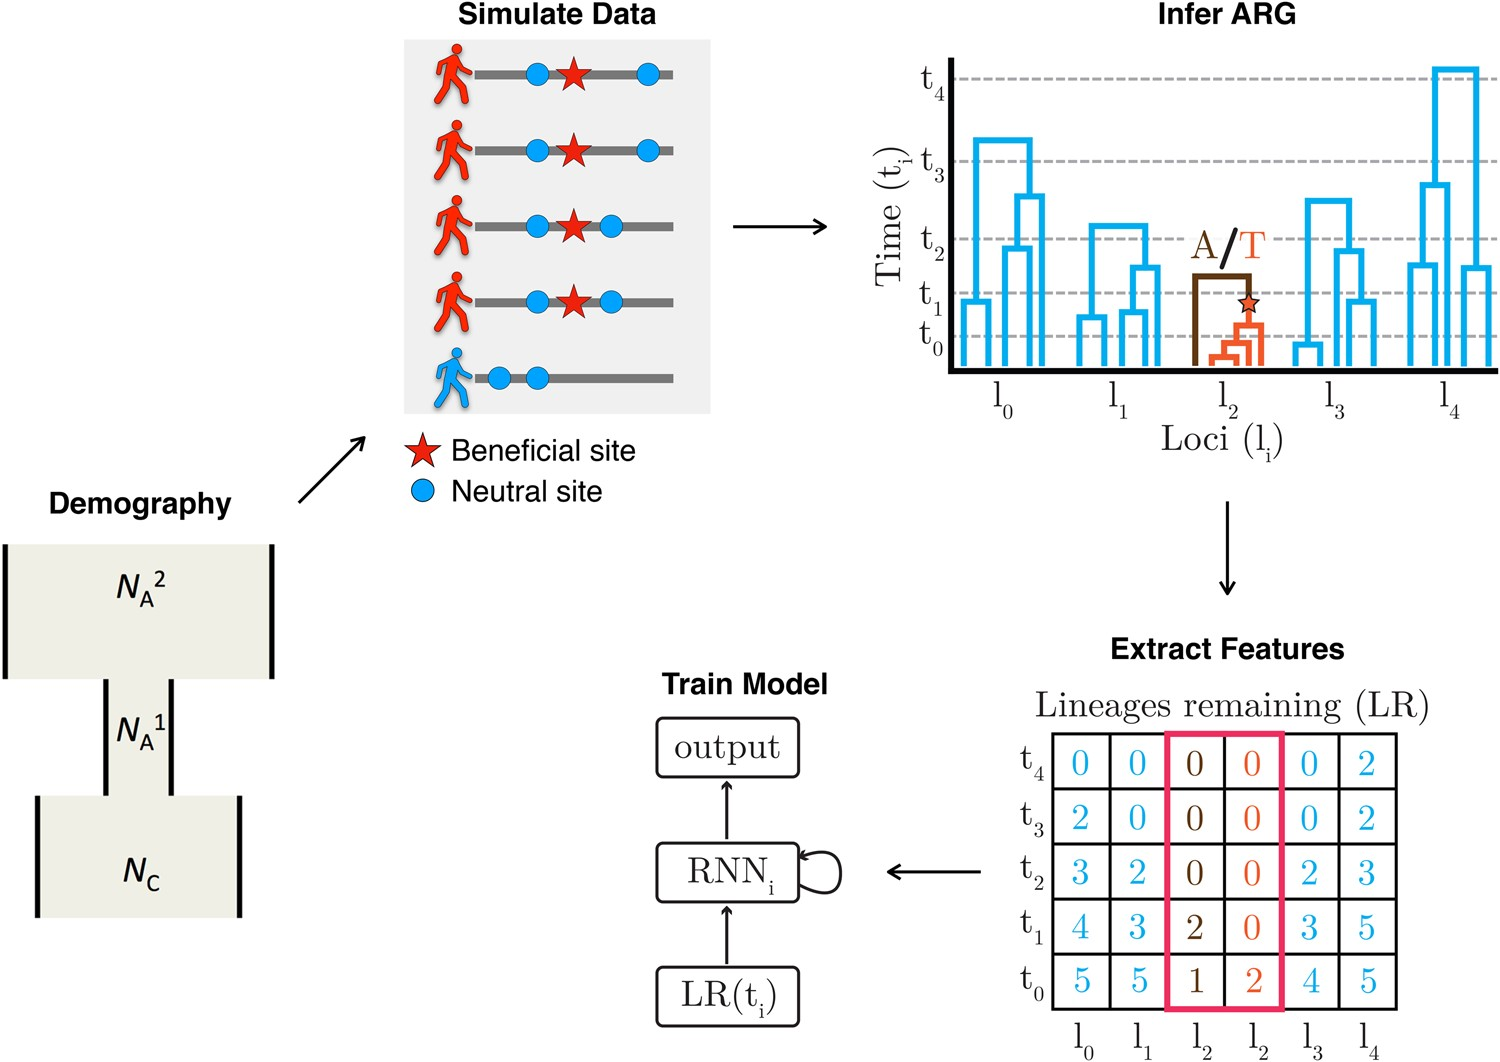
\includegraphics[width=\textwidth]{SIA_figs/SIA_F1.jpeg}
    \caption[A high-level framework for automating the detection of selective sweeps.]{\textbf{A high-level framework for automating the detection of selective sweeps.} We first estimate the demographic history for the population of interest, then based on the estimated demographic history, we simulate neutral regions and sweeps using the discoal simulator (\cite{kern_discoal_2016}). We proceed with \ac{ARG} inference and then extract \ac{ARG}-level statistics from each simulated region. The \ac{ARG}-level statistics are used as features for a deep-learning \ac{RNN} model. Finally, the trained model is applied to the empirical data to infer sweeps, selection coefficients, and \ac{AF} trajectories.}
    \label{fig:SIA-F1}
\end{figure}

\section{Results}
\subsection{Methodological overview}
\ac{SIA} is based on \iac{RNN} that is trained to predict selection at a genomic site from genealogical features at that site of interest and nearby sites (see \nameref{methods} for detailed descriptions; see Fig. \ref{fig:SIA-F1} for a conceptual overview of \ac{SIA}; and Fig. \href{https://academic.oup.com/mbe/article/39/1/msab332/6433161#supplementary-data}{S1} online for an illustration of \ac{ARG} features and the \ac{RNN} architecture). Based on the demography of a particular population of interest, training data including genomic regions under various strengths of selection are simulated. The \ac{ARG} is then inferred from each simulated data set. \ac{ARG}-level statistics are extracted at the site under selection (or a neutral site) as features to be used as input to the deep-learning model. Specifically, we use lineage counts at a set of discrete time points as a fixed-dimension encoding of a genealogy. The encoding of the genealogy at the focal site as well as similar encodings of flanking genealogies constitute the feature vector for that site. \ac{SIA} uses \iac{LSTM} architecture, designed specifically to handle the temporal nature of the feature set. The \ac{LSTM} unrolls temporally such that the lineage counts at each time point are fed to the network iteratively. Finally, the model trained on simulations is applied to \acp{ARG} inferred from empirical data to identify sweeps, infer selection coefficients, and \ac{AF} trajectories.

\subsection{Classification of sweeps}
We first compared \ac{SIA} with several existing methods, including the Tajima’s D (\cite{tajima_statistical_1989}) and H1 (\cite{garud_recent_2015}) summary statistics, iHS (\cite{voight_map_2006}), a genealogy-based statistic (\cite{speidel_method_2019}), and a summary-statistic-based \ac{ML} method (\cite{schrider_shic_2016,kern_diploshic_2018}) (see \nameref{methods}), in the classification task of distinguishing hard sweeps from neutrally evolving regions. Our performance comparison was conducted across 16 combinations of selection coefficients and segregating allele frequencies such that the beneficial site was subjected to selection ranging from weak to strong, resulting in low to high derived allele frequencies (\acsu{DAF}s). Because a priori we expected sweep sites with lower selection coefficients and lower \acp{DAF} to be harder to detect, we performed a stratified analysis of \ac{SIA}’s performance by selection coefficient and \ac{DAF}. Figure \ref{fig:SIA-F2} reports the \acf{ROC} curves using simulations based on the CEU demographic model (\cite{tennessen_evolution_2012}) where inferred genealogies were used as input to \ac{SIA} to account for gene tree uncertainty. As expected, all methods tended to perform better in a regime with higher selection coefficients and \acp{DAF}, as indicated by increasing values of the \ac{AUROC} statistic from left to right (increasing selection) and from top to bottom (increasing \ac{DAF}). \ac{SIA} outperformed the other methods across model conditions, with a more pronounced performance advantage for sites under weaker selection and segregating at lower \acp{DAF} (Fig. \ref{fig:SIA-F2}). For each given selection coefficient, the \ac{AUROC} of the Relate tree statistic (shown in red in Fig. \ref{fig:SIA-F2}), which measures how unlikely it is that the observed expansion of the derived lineages is purely due to genetic drift, did not substantially improve as the \ac{DAF} increased. Alleles at higher frequency tend to be older and subjected to drift over longer periods, which may lead to reduced power for Relate to distinguish lineage expansion under selection from the neutral expectation. Consequently, although the \ac{ARG}-based methods \ac{SIA} and Relate both outperformed other methods at low \acp{DAF}, \ac{SIA} was alone in maintaining this advantage at higher \acp{DAF}.

\begin{figure}%[h]
    \centering
    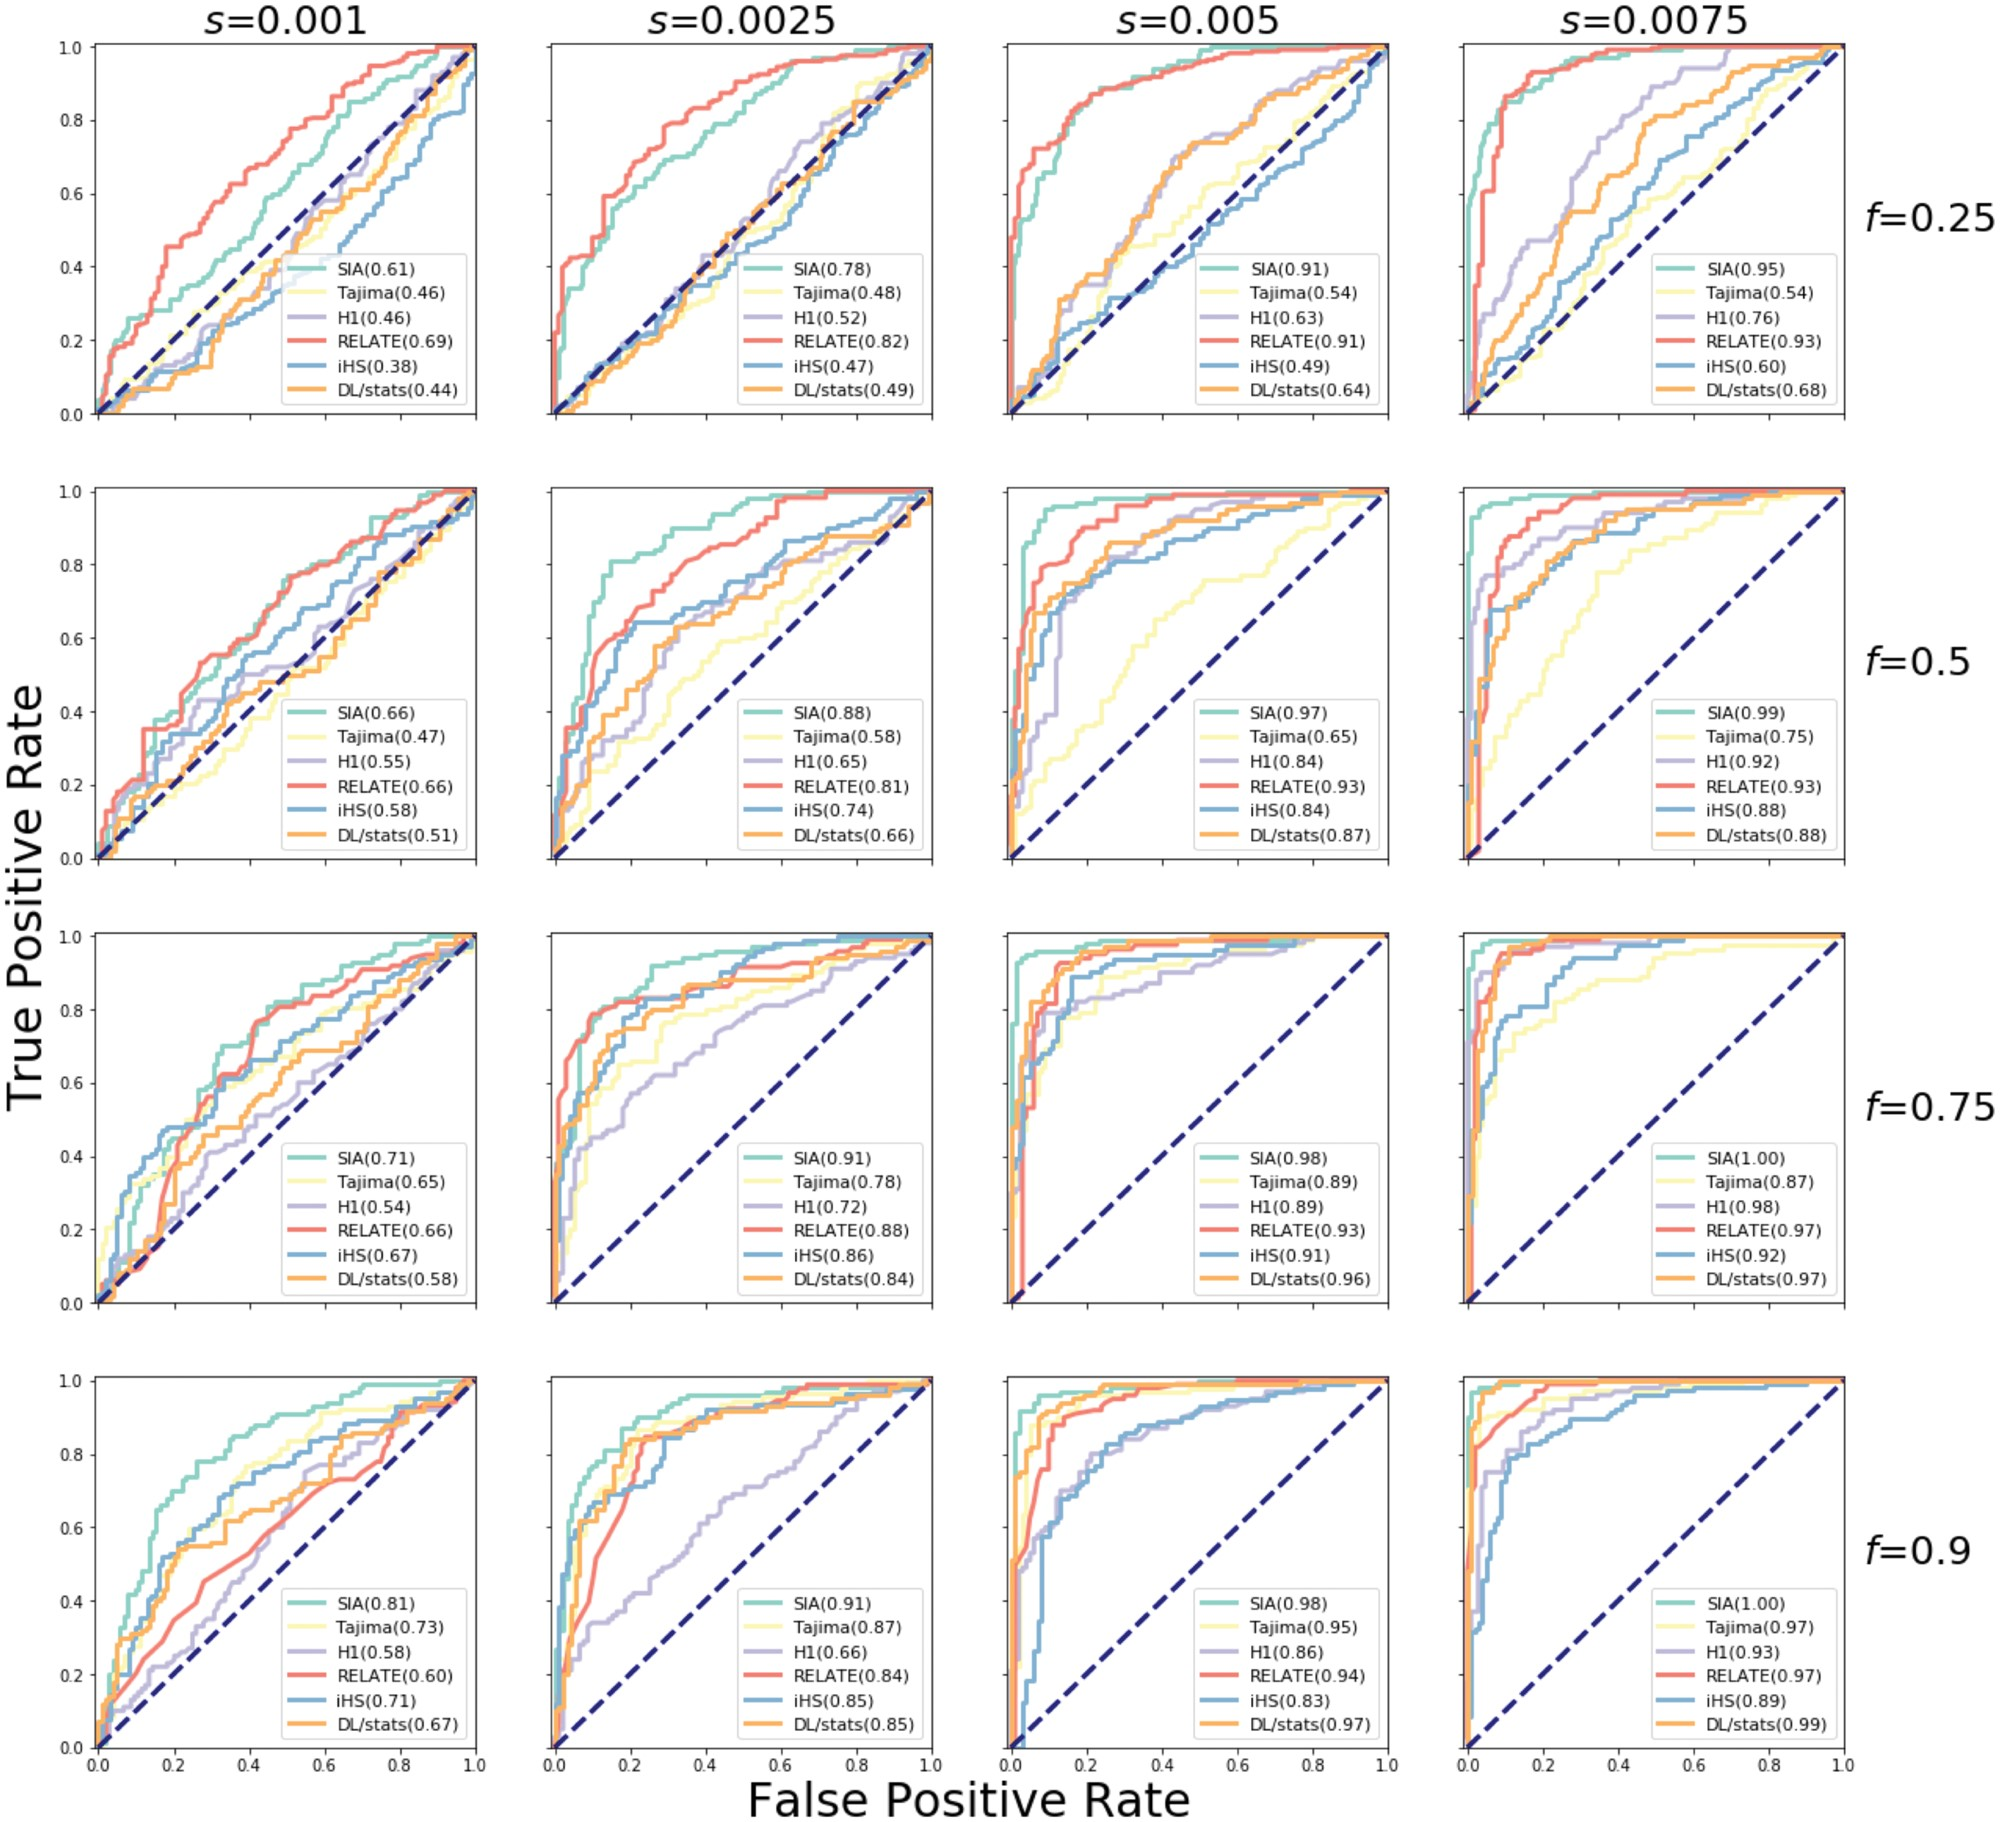
\includegraphics[width=\textwidth]{SIA_figs/SIA_F2.jpeg}
    \caption[Classification performance of \ac{SIA} and other methods on simulated data.]{\textbf{Classification performance of \ac{SIA} and other methods on simulated data.} Sequence data were simulated under a variety of selection regimes (\textit{s}, shown horizontally) and \acp{DAF} for the beneficial mutation under selection (\textit{f}, shown vertically) (see \nameref{methods} for more details). The prediction task distinguished neutral regions and sweeps. The methods were tested on a set of 200 regions per panel (100 per class), and the \ac{ROC} curve records the \acf{TP} rate as a function of the \acf{FP} rate. The curve is obtained by varying the prediction threshold from 0 to 1 and recording for each threshold the number of regions correctly assigned (\acp{TP}) or misassigned (\acp{FP}) as positives (with prediction probability above the threshold). The performance of each method was evaluated based on the area under its \ac{ROC} curve, or \ac{AUROC} (shown in parenthesis in figure legend). Note that inferred genealogies were used as input to \ac{SIA}.}
    \label{fig:SIA-F2}
\end{figure}

In addition, we validated the ability of \ac{SIA} to classify genomic regions with additional test sets simulated under a demographic model for southern capuchinos, a group of songbirds in which we previously identified and characterized many examples of sweeps (\cite{hejase_genomic_2020}), finding a predominance of “soft” rather than “hard” sweeps (meaning that they tend to be based on standing genetic variation rather than new mutations; see \nameref{methods}). Figure \href{https://academic.oup.com/mbe/article/39/1/msab332/6433161#supplementary-data}{S2} online reports the \ac{ROC} curves for the task of distinguishing partial soft sweeps from neutral regions. Despite soft sweeps being harder to detect, the classifier achieved good performance in the moderate-to-strong selection regimes ($s=0.005$ and $s=0.0075$) where the accuracy ranged between 82\% and 96\%, a substantial improvement over the previous accuracy of 56\% (\cite{hejase_genomic_2020}). \ac{SIA} performed particularly well in identifying partial soft sweeps when the site under selection was at a high segregating frequency. For example, at segregating frequencies of 0.75 and 0.9, the performance of \ac{SIA} ranged between 80\% and 96\% across a variety of selection regimes ($s=0.0025$, 0.005, and 0.0075). The performance of \ac{SIA} degraded somewhat for weak selection ($s=0.001$) with an accuracy ranging between 63\% and 74\%.

\subsection{Selection coefficient inference using true gene trees}
We assessed the performance of \ac{SIA} in correctly predicting the selection coefficient and compared it with CLUES (\cite{stern_approximate_2019}). Like \ac{SIA}, CLUES uses local genealogies based on the \ac{ARG} to infer a selection coefficient. However, CLUES calculates the likelihood of the genealogy analytically using \iac{HMM}, and does not rely on simulated training data. In addition, CLUES uses a single genealogy at the focal site, whereas \ac{SIA} additionally considers flanking trees.

We began by supplying both methods with true genealogies, in order to later disentangle the error deriving from the \ac{ARG} inference step from other sources of error (see \nameref{discussion}). We found that \ac{SIA} identified regions under neutrality with approximately no bias (median inferred $s=7.5\times 10^{-5}$; Fig. \ref{fig:SIA-F3}). Similarly, \ac{SIA} correctly inferred the selection coefficient for regions under moderate to strong selection ($s \in \{0.0025, 0.005, 0.0075, 0.01\}$) with the median inferred $s$ deviated from the true $s$ by at most 3\%. On the other hand, \ac{SIA} somewhat underestimated the selection coefficient (median inferred $s = 0.00037$) for the weak selection regime (true $s = 0.001$), likely owing to limits in the training set within that selection regime (see \nameref{discussion}). We further binned the results by segregating frequency and selection coefficient and found that, in general, the variance in estimates of $s$ for \ac{SIA} (as well as CLUES) tended to decrease as the segregating frequency of the beneficial allele increased (Fig. \href{https://academic.oup.com/mbe/article/39/1/msab332/6433161#supplementary-data}{S3 online}).

\begin{figure}[h]
    \centering
    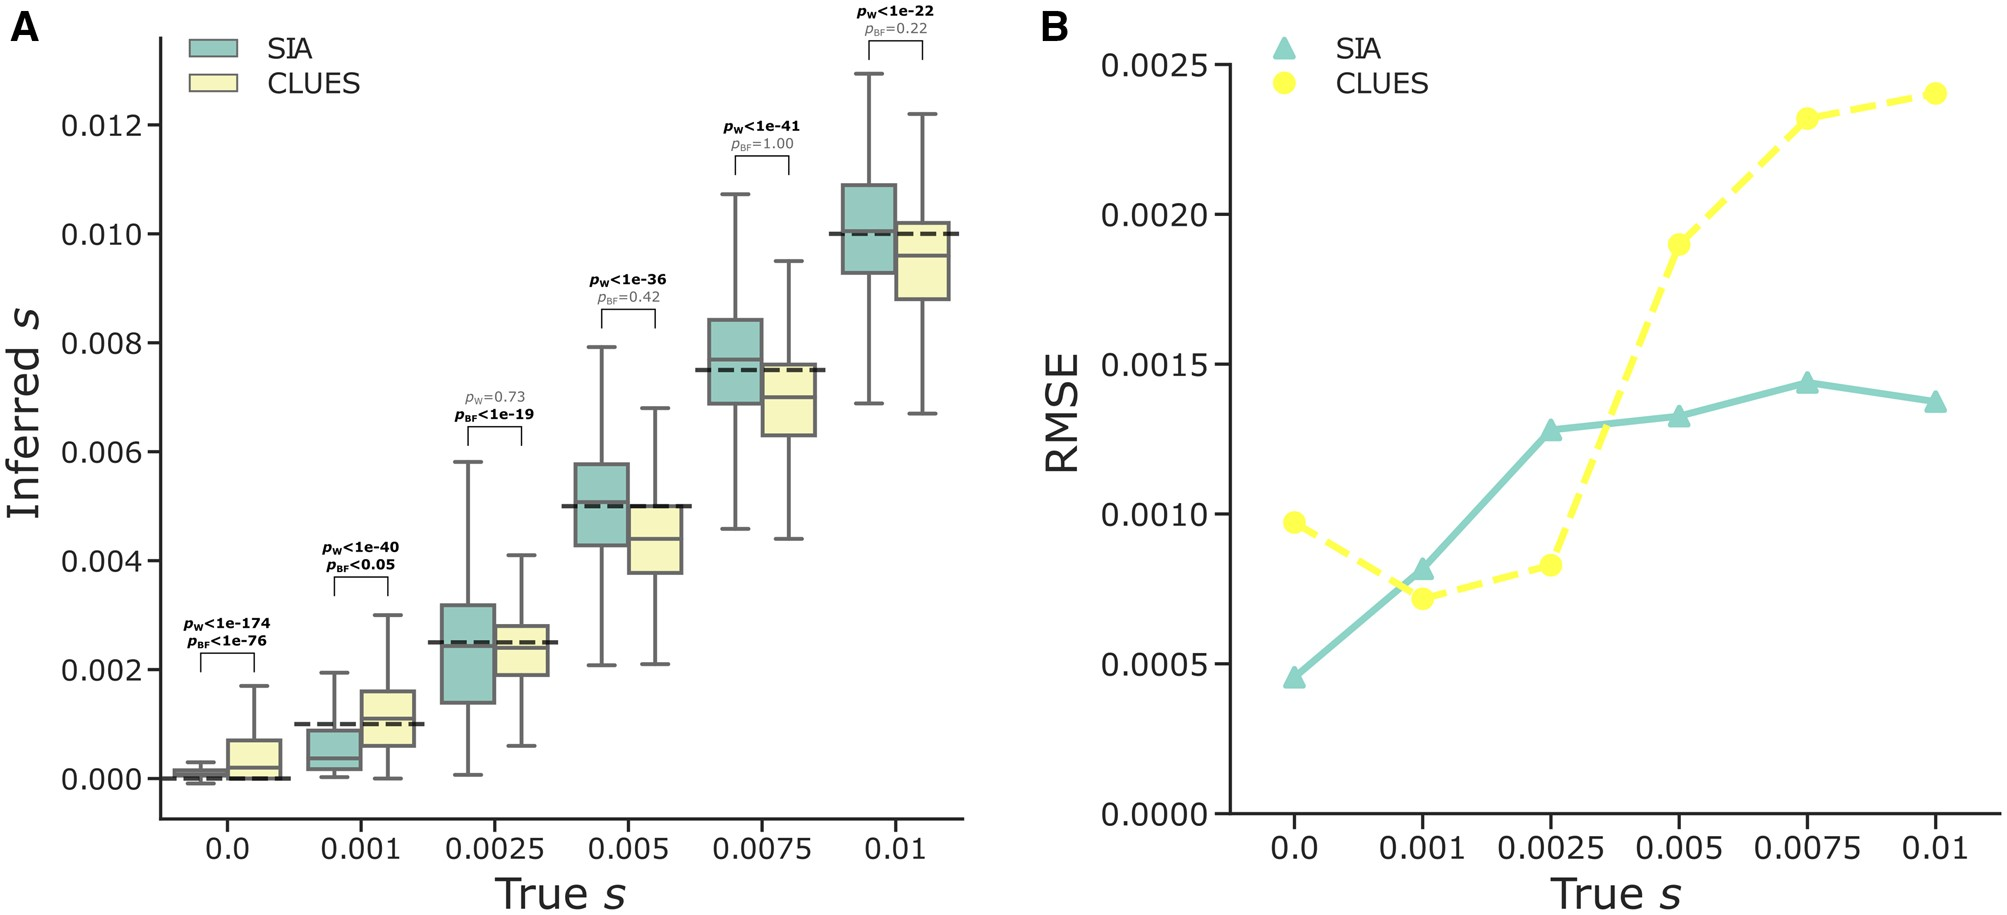
\includegraphics[width=\textwidth]{SIA_figs/SIA_F3.jpeg}
    \caption[Predictions of selection coefficients on simulated regions using \ac{SIA} and CLUES based on true genealogies.]{\textbf{Predictions of selection coefficients on simulated regions using \ac{SIA} and CLUES based on true genealogies.} \textbf{(\textit{A})} The distribution of inferred selection coefficients for each method under each model condition are reported using a box plot. The box plot for each method reports these five statistics (from bottom to top): minimum, first quartile, median, third quartile, and maximum. The $y$-axis shows the inferred selection coefficient, whereas the $x$-axis shows the true selection coefficient. The dashed-black line indicates the true selection coefficient for each model condition. The simulations are based on the CEU demographic model and true genealogies were used as input to both methods. Each model condition (i.e., box plot) represents a set of 400 independent simulations. The mean ranks and variances of the distributions of inferred $s$ were compared using the Wilcoxon signed-rank test ($p_\mathrm{W}$) and the Brown–Forsythe test ($p_{\mathrm{BF}}$), respectively. \textbf{(\textit{B})} The \acf{RMSE} for each method under each model condition evaluated on 400 independent simulations.}
    \label{fig:SIA-F3}
\end{figure}

CLUES performed roughly similarly to \ac{SIA} in this experiment, but tended to slightly overestimate $s$ for the neutral regions (i.e., true $s=0$) and underestimate $s$ for the moderate to high selection regimes (i.e., true $s=$ 0.005, 0.0075, and 0.01). Under these conditions, \ac{SIA}’s median predictions of $s$ were noticeably closer to the true values (Fig. \ref{fig:SIA-F3}A). At the same time, CLUES performed slightly better than \ac{SIA} in weak selection regimes (i.e., true $s=$ 0.001 and 0.0025) (Fig. \ref{fig:SIA-F3}). Overall, \ac{SIA} (\ac{RMSE} = $9.52\times 10^{-4}$) achieved a lower error in estimating s than CLUES (\ac{RMSE} = $1.44\times 10^{-3}$), when true genealogies were used as input to both methods (Wilcoxon signed-rank test for difference in mean of squared error, $P=1.25\times 10^{-42}$). This finding potentially reflects the benefit of linkage information utilized by \ac{SIA} through the additional flanking genealogies (see \nameref{discussion}).

\subsection{Selection coefficient inference using inferred gene trees}
To account for gene-tree uncertainty, we next used \acp{ARG} inferred with Relate, which is scalable to the size of the training data set for \ac{SIA} (see \nameref{methods}), as input to \ac{SIA} and CLUES and compared their performance on CEU simulations. Using a reduced sample size of 32 haplotypes, we additionally compared \ac{SIA} with CLUES supplied with genealogies sampled using ARGweaver. Furthermore, we compared both methods with a supervised \ac{ML} method, ImaGene (see \href{https://academic.oup.com/mbe/article/39/1/msab332/6433161#supplementary-data}{Fig. S23 online}), that operates directly on an image of the alignment itself. ImaGene does not require gene trees as input and instead uses \iac{CNN} to perform dimensionality reduction of the sequence alignment, allowing for accurate and efficient classification and regression.

Overall, we found that \ac{SIA} and ImaGene outperformed CLUES in these experiments (Fig. \ref{fig:SIA-F4}). CLUES tended to underestimate selection coefficients for the moderate-to-strong selection regimes, to a greater extent compared with the case where true genealogies were used for inference (Figs. \ref{fig:SIA-F3}A and \ref{fig:SIA-F4}A). This decrease in performance of CLUES evidently derives from error at the \ac{ARG} reconstruction step. \ac{SIA}, on the other hand, appeared to be more robust to the same \ac{ARG} reconstruction error, and maintained an advantage even when CLUES was provided posterior samples of genealogies from ARGweaver (Fig. \href{https://academic.oup.com/mbe/article/39/1/msab332/6433161#supplementary-data}{S5 online}). ImaGene performed remarkably similarly to \ac{SIA}, given that it relies solely on the sequence alignment. \ac{SIA} exhibited lower error at neutral sites and sites with low-to-moderate values of $s$, whereas ImaGene prevailed at sites under strong selection (Fig. \ref{fig:SIA-F4}B). Nevertheless, \ac{SIA} showed a slightly smaller overall \ac{RMSE} ($2.75\times 10^{-3}$) compared with ImaGene ($2.91\times 10^{-3}$) (Wilcoxon signed-rank test, $P = 6.18\times 10^{-38}$), and in particular, \ac{SIA} produces estimates of $s$ much closer to 0 for neutral loci. Notably, in this case both \ac{SIA} and ImaGene were trained with simulations under the same uniform distribution of $s$ values (see \nameref{methods}). A different choice of training distribution could impact their performance across selection regimes (see \nameref{discussion}). Furthermore, we binned the results of these methods by both the segregating frequency and the selection coefficient (see Fig. \href{https://academic.oup.com/mbe/article/39/1/msab332/6433161#supplementary-data}{S4 online}) and again found that in general they exhibit higher variance under low segregating frequency of the beneficial allele. As before, we also tested our regression framework on true and inferred gene trees of test sets simulated under the \textit{Sporophila hypoxantha} demographic model (see Fig. \href{https://academic.oup.com/mbe/article/39/1/msab332/6433161#supplementary-data}{S6 online}). We found that \ac{SIA} was approximately unbiased for the moderate ($s=0.005$) and high ($s=0.01$) selection regimes but appeared to overestimate the selection coefficient for regions under weak selection ($s=$ 0.001 and 0.0025), when both true and inferred genealogies were used as input. Furthermore, \ac{SIA} appeared to overestimate the selection coefficient for neutral regions when inferred gene trees were used as input, whereas it was approximately unbiased for true gene trees.

\begin{figure}[h]
    \centering
    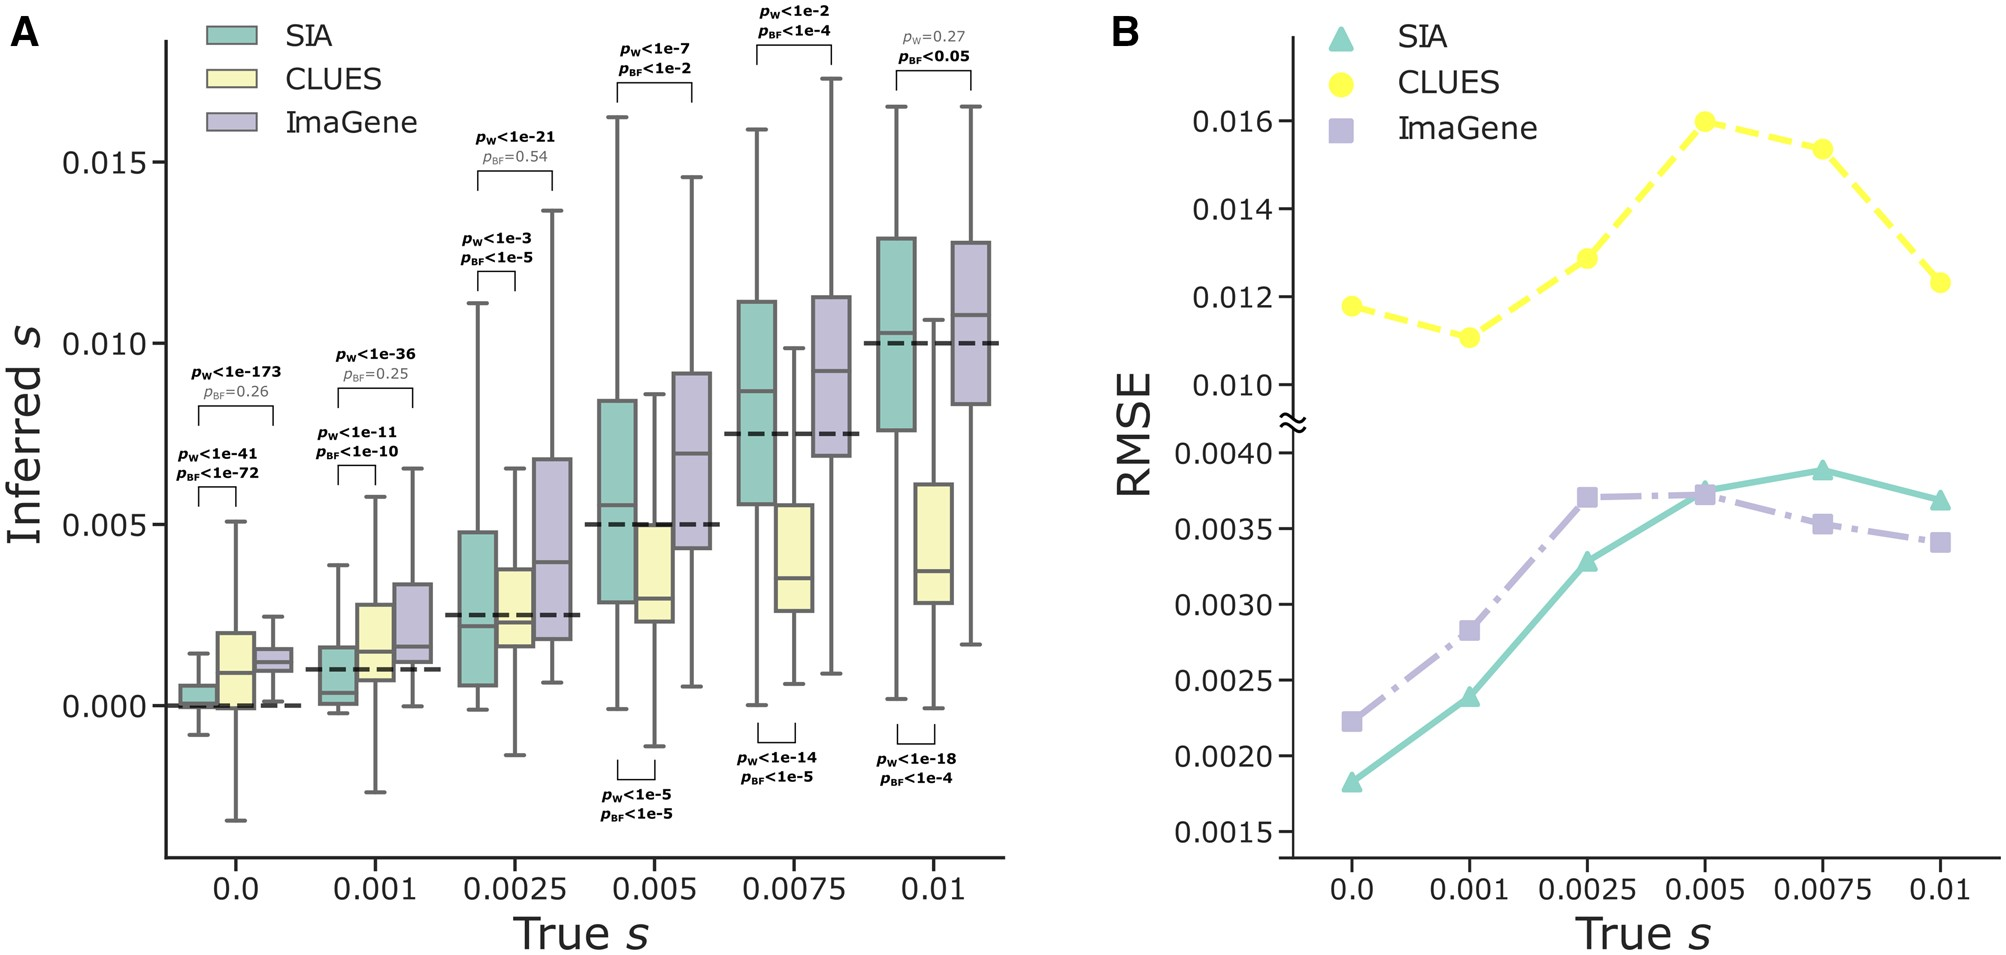
\includegraphics[width=\textwidth]{SIA_figs/SIA_F4.jpeg}
    \caption[Predictions of selection coefficient on simulated regions using \ac{SIA} and CLUES based on inferred genealogies, and ImaGene.]{\textbf{Predictions of selection coefficient on simulated regions using \ac{SIA} and CLUES based on inferred genealogies, and ImaGene.} \textbf{(\textit{A})} The distribution of inferred selection coefficients and \textbf{(\textit{B})} \ac{RMSE} for each method under each model condition. The simulations are based on the CEU demographic model where inferred genealogies were used as input to \ac{SIA} and CLUES, whereas sequence alignments were used as input to ImaGene. Figure layout and description are otherwise similar to Figure \ref{fig:SIA-F3}.}
    \label{fig:SIA-F4}
\end{figure}

\subsection{Performance on selection coefficient prediction with different sample sizes}
To explore the tradeoffs associated with the use of larger data sets, we examined the performance of \ac{SIA} under different sample sizes, assuming a constant-sized demographic model ($N_e = 10,000$). Figure \href{https://academic.oup.com/mbe/article/39/1/msab332/6433161#supplementary-data}{S7 online} shows the error in selection coefficient inference on a held-out test set, stratified by the age of the allele (Fig. \href{https://academic.oup.com/mbe/article/39/1/msab332/6433161#supplementary-data}{S7A and B online}) and present-day \ac{DAF} (Fig. \href{https://academic.oup.com/mbe/article/39/1/msab332/6433161#supplementary-data}{S7C and D online}) at the site of interest. We observed that sites with low frequency (\ac{AF} $<0.33$) and more recent (onset $<0.2\times 2N_e$ generations) alleles experience the most significant reduction in error as sample size increases. Notably, the performance of \ac{SIA} on more ancient alleles (onset $>0.2\times 2N_e$ generations) had little to no improvement as the sample size increased from 32 to 254. These observations are in line with the expectation that having more samples improves the chance of capturing low-frequency alleles, but provides limited information about more ancient events. The reason for this age-dependency is that, looking backwards in time, most lineages coalesce rapidly and only a few survive to more ancient epochs, in a manner that depends only weakly on the sample size. It may be useful to consider these observations when choosing the sample size for use in studying selection in a particular context (see \nameref{discussion}).

\subsection{Inference of \ac{AF} trajectory}
We further adapted the deep-learning architecture of \ac{SIA} to model the \ac{AF} trajectory at a site by retaining the output of the \ac{LSTM} at each time point (Fig. \href{https://academic.oup.com/mbe/article/39/1/msab332/6433161?login=true#supplementary-data}{S1 online}; see \nameref{methods}). We then evaluated the performance of \ac{SIA} in the inference of the \ac{AF} trajectory using simulations under the CEU demography across a range of selection coefficients and current \acp{DAF}. \ac{SIA} was largely able to capture the expected trend of more rapidly increasing \ac{AF} under stronger selection (Figs. \href{https://academic.oup.com/mbe/article/39/1/msab332/6433161?login=true#supplementary-data}{S8 and S11 online}). In addition, \ac{AF} estimates by \ac{SIA} using both true and inferred genealogies were generally unbiased, although \ac{AF} at more recent time points tended to be slightly underestimated when data was simulated under weaker selection. \ac{AF} estimates also appeared to be more accurate in terms of variance for alleles under stronger selection (Figs. \href{https://academic.oup.com/mbe/article/39/1/msab332/6433161?login=true#supplementary-data}{S9 and S12 online}). As expected, the variance of \ac{AF} estimates tended to increase going further back in time (Figs. \href{https://academic.oup.com/mbe/article/39/1/msab332/6433161?login=true#supplementary-data}{S9 and S12 online}). We also observed that overall \ac{SIA} tended to produce more accurate \ac{AF} estimates than CLUES (Figs. \href{https://academic.oup.com/mbe/article/39/1/msab332/6433161?login=true#supplementary-data}{S9 and S10 online}).

\subsection{Model performance on simulations with mis-specified demographic models}
To evaluate the robustness of \ac{SIA} to mismatches between the demographic parameters used for simulating training data and the true underlying demography of real data, we tested the method on the selection-coefficient inference task with data sets simulated under a range of alternative parameters. Each aspect of this model mis-specification was assessed independently of the others. In particular, the mis-specified data sets contained simulations under 1) combinations of population mutation ($\theta$) and recombination ($\rho$) rates sampled beyond the range used for the training data (Figs. \href{https://academic.oup.com/mbe/article/39/1/msab332/6433161?login=true#supplementary-data}{S13 and S16 online}); 2) various alternative demographic scenarios (Figs. \href{https://academic.oup.com/mbe/article/39/1/msab332/6433161?login=true#supplementary-data}{S14, S17, and S19 online}); and 3) various effective population sizes (Figs. \href{https://academic.oup.com/mbe/article/39/1/msab332/6433161?login=true#supplementary-data}{S15 and S18 online}). We compared the performance of \ac{SIA} on these mis-specified data sets with that of CLUES (\cite{stern_approximate_2019}), supplying both methods with the true genealogies. We consider CLUES the “silver standard” when it comes to robustness because it is unsupervised and therefore should not be susceptible to mis-specified training data compared with supervised learning methods such as \ac{SIA}. Overall, we found that both CLUES and \ac{SIA} were reasonably robust to model mis-specification (Figs. \href{https://academic.oup.com/mbe/article/39/1/msab332/6433161?login=true#supplementary-data}{S13–S15 online}), although the performance of both methods inevitably declined when tested on severely mis-specified data (Fig. \href{https://academic.oup.com/mbe/article/39/1/msab332/6433161?login=true#supplementary-data}{S15 online}). Interestingly, \ac{SIA} tended to overestimate selection coefficient when the true $N_e$ was much smaller than that used for training, and underestimate it when the true $N_e$ was much larger, whereas CLUES did the opposite (Fig. \href{https://academic.oup.com/mbe/article/39/1/msab332/6433161?login=true#supplementary-data}{S15 online}). Because the CLUES likelihood model of \ac{AF} transition is parameterized by the population-scaled selection coefficient ($\alpha = 2Ns$), a larger $N_e$ likely appears to CLUES as equivalent to a higher $s$. On the other hand, features used by \ac{SIA} capture broad information of coalescence and linkage in the \ac{ARG}, and therefore can be distorted by mis-specified $N_e$ in more subtle ways (see \nameref{discussion}). Using the same mis-specified data set, we also ran \ac{SIA} with Relate-inferred genealogies and compared its performance with that of the genotyped-based deep-learning model ImaGene (\cite{flagel_unreasonable_2019,torada_imagene_2019}). In general, \ac{SIA} appeared to be more robust to model mis-specifications, achieving an overall \ac{RMSE} of 0.00362, 0.00318, and 0.00374 in the mis-specified $\theta/\rho$, demography, and $N_e$ experiments, respectively, compared with ImaGene, whose \ac{RMSE} was 0.00416, 0.00330, and 0.00462 in the corresponding experiments (Figs. \href{https://academic.oup.com/mbe/article/39/1/msab332/6433161?login=true#supplementary-data}{S16–S18 online}). The advantage of \ac{SIA} was particularly noticeable in cases of mis-specified demographic parameters (Figs. \href{https://academic.oup.com/mbe/article/39/1/msab332/6433161?login=true#supplementary-data}{S17 and S18 online}). Notably, \ac{SIA} exhibited reduced bias when working with inferred genealogies compared with true genealogies, under conditions of extremely mismatched $N_e$ (compare Figs. \href{https://academic.oup.com/mbe/article/39/1/msab332/6433161?login=true#supplementary-data}{S15 and S18 online}).

\subsection{Model prediction at genomic loci of interest in CEU population}
We then applied the \ac{SIA} model to identify selective sweeps and infer selection coefficients at selected genomic loci in the 1000 Genomes CEU population. These loci included the canonical example of selection at the \textit{MCM6} gene, which regulates the neighboring \textit{LCT} gene and contributes to the lactase persistence trait (\cite{bersaglieri_genetic_2004}), the \textit{ABCC11} gene regulating earwax production, several pigmentation-related genes, as well as genes associated with obesity, diabetes and addiction (Table \ref{tab:SIA-T1}).


\begin{sidewaystable}
    
    \centering
    \caption{List of genomic loci of interest along with their \acfp{DAF}, sweep probabilities, and selection coefficients inferred by \ac{SIA} in the 1000 Genomes CEU population.}
    \vspace{5mm}
    \begin{tabular}{m{6cm} r r r r r c}
        \hline
        \textbf{Gene} & \textbf{SNP ID} & \textbf{Chr} & \textbf{Position}* & \textbf{\ac{DAF}} & $P_{\mathrm{\textbf{sweep}}}$ & \textbf{Selection coefficient (95\% CI)} \\
        \hline
        \textit{LCT} (\cite{bersaglieri_genetic_2004}) & rs4988235 & 2 & 136608646 & 0.74 & 0.999 & [0.01019, 0.01056] \\
        \textit{OCA2} (\cite{han_genome-wide_2008,sturm_single_2008}) & rs12913832 & 15 & 28365618 & 0.77 & 0.750 & [0.00539, 0.00575] \\
        \textit{MC1R} (\cite{sulem_genetic_2007,han_genome-wide_2008}) & rs1805007 & 16 & 89986117 & 0.12 & 0.949 & [0.00362, 0.00384] \\
        \textit{ABCC11} (\cite{yoshiura_snp_2006}) & rs17822931 & 16 & 48258198 & 0.13 & 0.620 & [0.00034, 0.00036] \\
        \textit{ASIP} (\cite{eriksson_web-based_2010}) & rs619865 & 20 & 33867697 & 0.12 & 0.777 & [0.00172, 0.00197] \\
        \textit{TYR} (\cite{sulem_genetic_2007,eriksson_web-based_2010}) & rs1393350 & 11 & 89011046 & 0.24 & 0.616 & [0.00085, 0.00135] \\
        \textit{KITLG} (\cite{sulem_genetic_2007}) & rs12821256 & 12 & 89328335 & 0.13 & 0.869 & [0.00183, 0.002] \\
        \textit{TYRP1} (\cite{kenny_melanesian_2012}) & rs13289810 & 9 & 12396731 & 0.37 & 0.144 & [0.00004, 0.00006] \\
        \textit{TTC3} (\cite{liu_digital_2010}) & rs1003719 & 21 & 38491095 & 0.62 & 0.011 & [0, 0] \\
        \textit{OCA2} & rs7495174 & 15 & 28344238 & 0.94 & 0.013 & [0, 0.00005] \\
        \textit{TCF7L2} (\cite{lyssenko_mechanisms_2007}) & rs7903146 & 10 & 114758349 & 0.69 & 0.035 & [0, 0] \\
        \textit{ANKK1} (\cite{spellicy_variant_2014}) & rs1800497 & 11 & 113270828 & 0.80 & 0.045 & [0, 0] \\
        \textit{FTO} (\cite{frayling_common_2007}) & rs9939609 & 16 & 53820527 & 0.56 & 0.011 & [0, 0] \\
        \hline
        \rowcolor{white} \multicolumn{7}{l}{*Genomic coordinates in GRCh37 (hg19) assembly}
    \end{tabular}
    \label{tab:SIA-T1}
\end{sidewaystable}

For \textit{LCT}, \ac{SIA} detected a strong signal of selection at the nearby \acs{SNP} that has been associated with the lactase persistence trait (rs4988235). At this \acs{SNP}, \ac{SIA} inferred a sweep probability close to 1 and a selection coefficient $>0.01$, making this one of the strongest signals of selection in the human genome. A close examination of the local genealogy at this site reveals a clear pattern indicative of a selective sweep––a burst of recent coalescence among the derived lineages (orange taxa are the lineages carrying the derived allele) is clearly visible from the tree (Fig. \ref{fig:SIA-F5}).

\begin{figure}
    \centering
    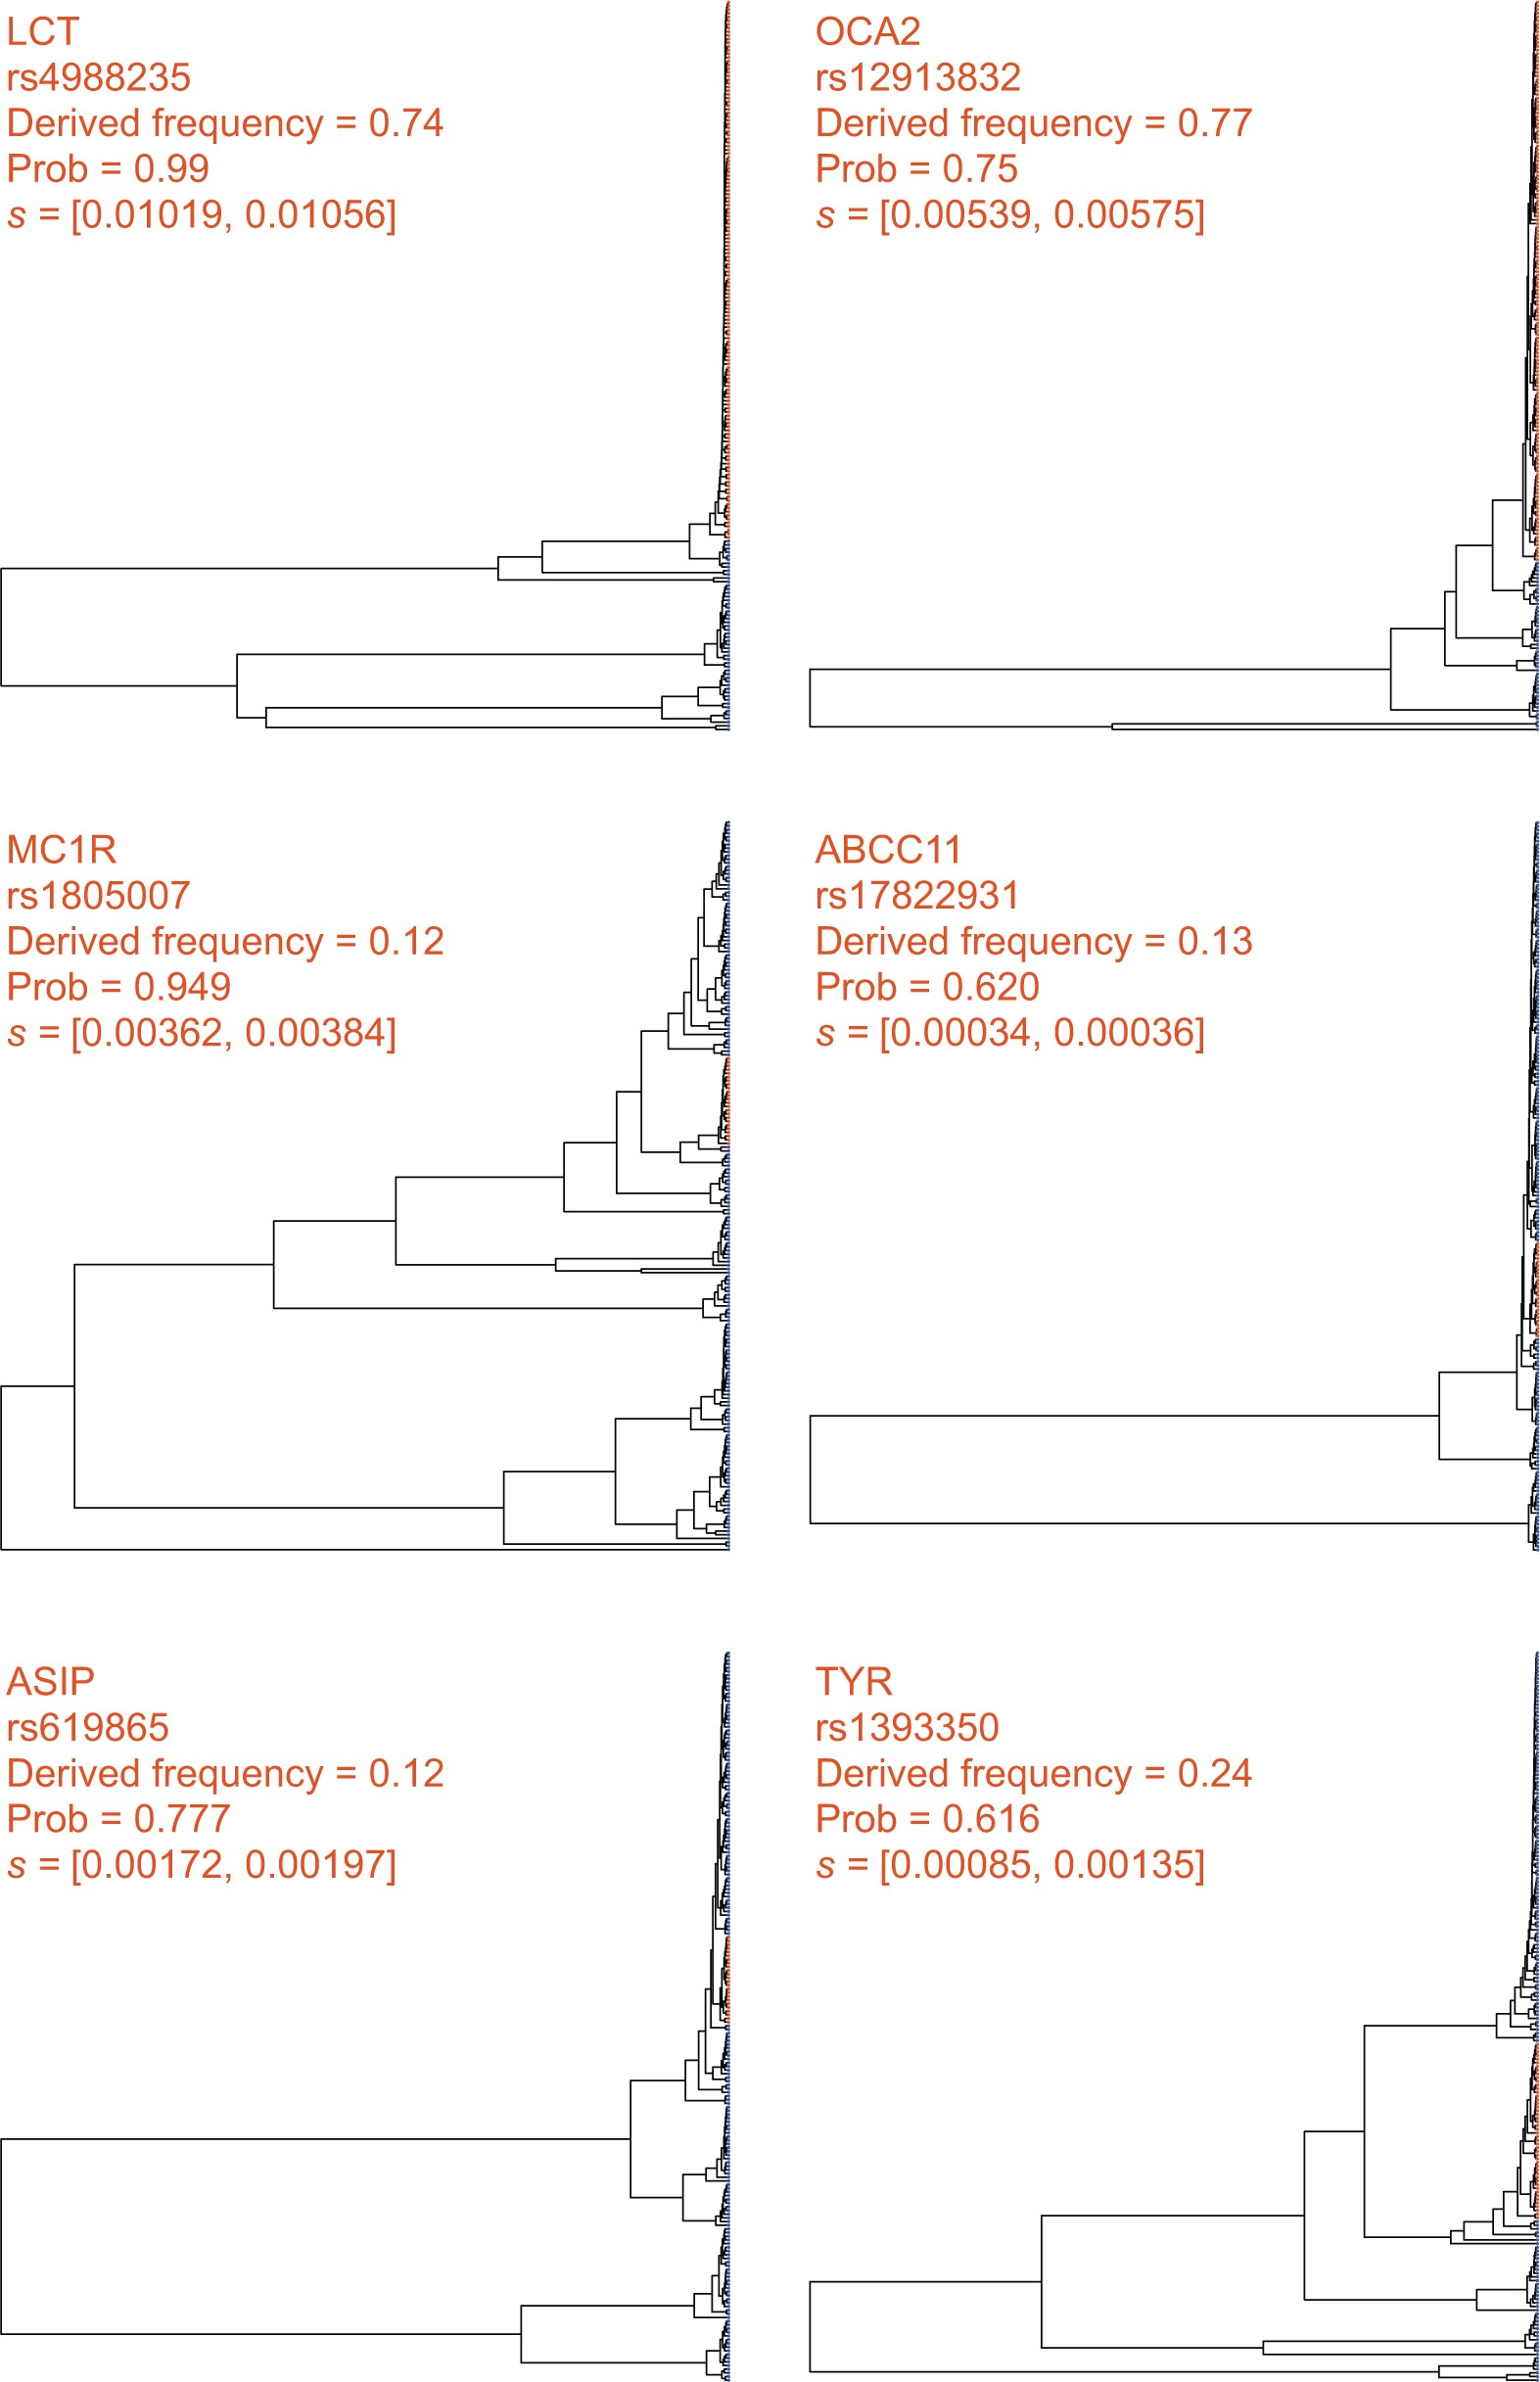
\includegraphics[scale=0.25]{SIA_figs/SIA_F5.jpeg}
    \caption[Local genealogies at six loci inferred to be under positive selection in the 1000 Genomes CEU population.]{\textbf{Local genealogies at six loci inferred to be under positive selection in the 1000 Genomes CEU population.} Gene name, RefSNP number, derived \ac{AF}, \ac{SIA}-inferred sweep probability and \ac{SIA}-inferred selection coefficient range for each locus are indicated at the top of each panel (see Table \ref{tab:SIA-T1} for more details). Taxa carrying the ancestral and derived alleles are colored in blue and orange, respectively.}
    \label{fig:SIA-F5}
\end{figure}

At a number of pigmentation genes (\cite{sulem_genetic_2007,han_genome-wide_2008,sturm_single_2008,liu_digital_2010,kenny_melanesian_2012}), \ac{SIA} detected signals of moderate selection, including \textit{MC1R} (rs1805007, $P_{\mathrm{sweep}} = 0.95$, $s \approx 0.0037$), \textit{KITLG} (rs12821256, $P_{\mathrm{sweep}} = 0.87$, $s \approx 0.0019$), \textit{ASIP} (rs619865, $P_{\mathrm{sweep}} = 0.78$, $s \approx 0.0019$), \textit{OCA2} (rs12913832, $P_{\mathrm{sweep}} = 0.75$, $s \approx 0.0056$), and \textit{TYR} (rs1393350, $P_{\mathrm{sweep}} = 0.62$, $s \approx 0.0011$). In addition, \ac{SIA} identified a weak signal of selection at a \acs{SNP} in the \textit{ABCC11} gene (rs17822931), which influences earwax and sweat production (\cite{yoshiura_snp_2006}), with a selection coefficient of around 0.00035. There are few other estimates for these genes available for comparison, but, notably, our estimate for \textit{LCT} of $s \approx 0.01$ is consistent with a previous estimate on the order of 0.01–0.1 (\cite{bersaglieri_genetic_2004}), and with recent studies of ancient DNA samples (\cite{mathieson_fads1_2018,mathieson_estimating_2020}) suggesting a value closer to 0.01. Our estimates suggest that selection at the pigmentation loci is considerably weaker than at \textit{LCT}, in contrast to previous estimates for these loci, which covered a wide range but were generally considerably larger (ranging from 0.02 to 0.1) (\cite{wilde_direct_2014}). Interestingly, CLUES estimated $s$ at the \textit{OCA2} locus to be on the order of 0.001 (roughly similar to \ac{SIA}’s estimate of 0.0056), but $s$ at the \textit{KITLG}, \textit{ASIP}, \textit{TYR} loci to be $>0.01$ (in comparison to \ac{SIA}’s considerably smaller estimates of 0.0019, 0.0019, and 0.0011) (\cite{stern_approximate_2019}). The apparent discrepancy between the estimates may be partially due to the fact that the two methods used samples from two different populations (CEU for SIA and GBR/British for CLUES).

On the other hand, SIA did not detect significant evidence of positive selection at several disease-associated loci (rs7903146/\textit{TCF7L2}, rs1800497/\textit{ANKK1}, and rs9939609/\textit{FTO}) or at several other pigmentation loci (rs13289810/\textit{TYRP1}, rs1003719/\textit{TTC3}, and rs7495174/\textit{OCA2}) (Table \ref{tab:SIA-T1}). Notably, allele frequencies at these six loci tend to be similar in African and European populations (\cite{marcus_visualizing_2017}), suggesting that they are not likely to be under strong environment-dependent positive selection, although it is possible that they have experienced very recent selective pressure that \ac{SIA} lacks the power to detect (see \nameref{discussion}). Notably, \textit{TYRP1} and \textit{TTC3} also lacked signals of selection in the CLUES analysis. Compared with the genealogies at sweep sites (Fig. \ref{fig:SIA-F5}), the trees at these putatively neutral loci lack the distinctive signature of recent bursts of coalescence among derived lineages (Fig. \ref{fig:SIA-F6}).

\begin{figure}
    \centering
    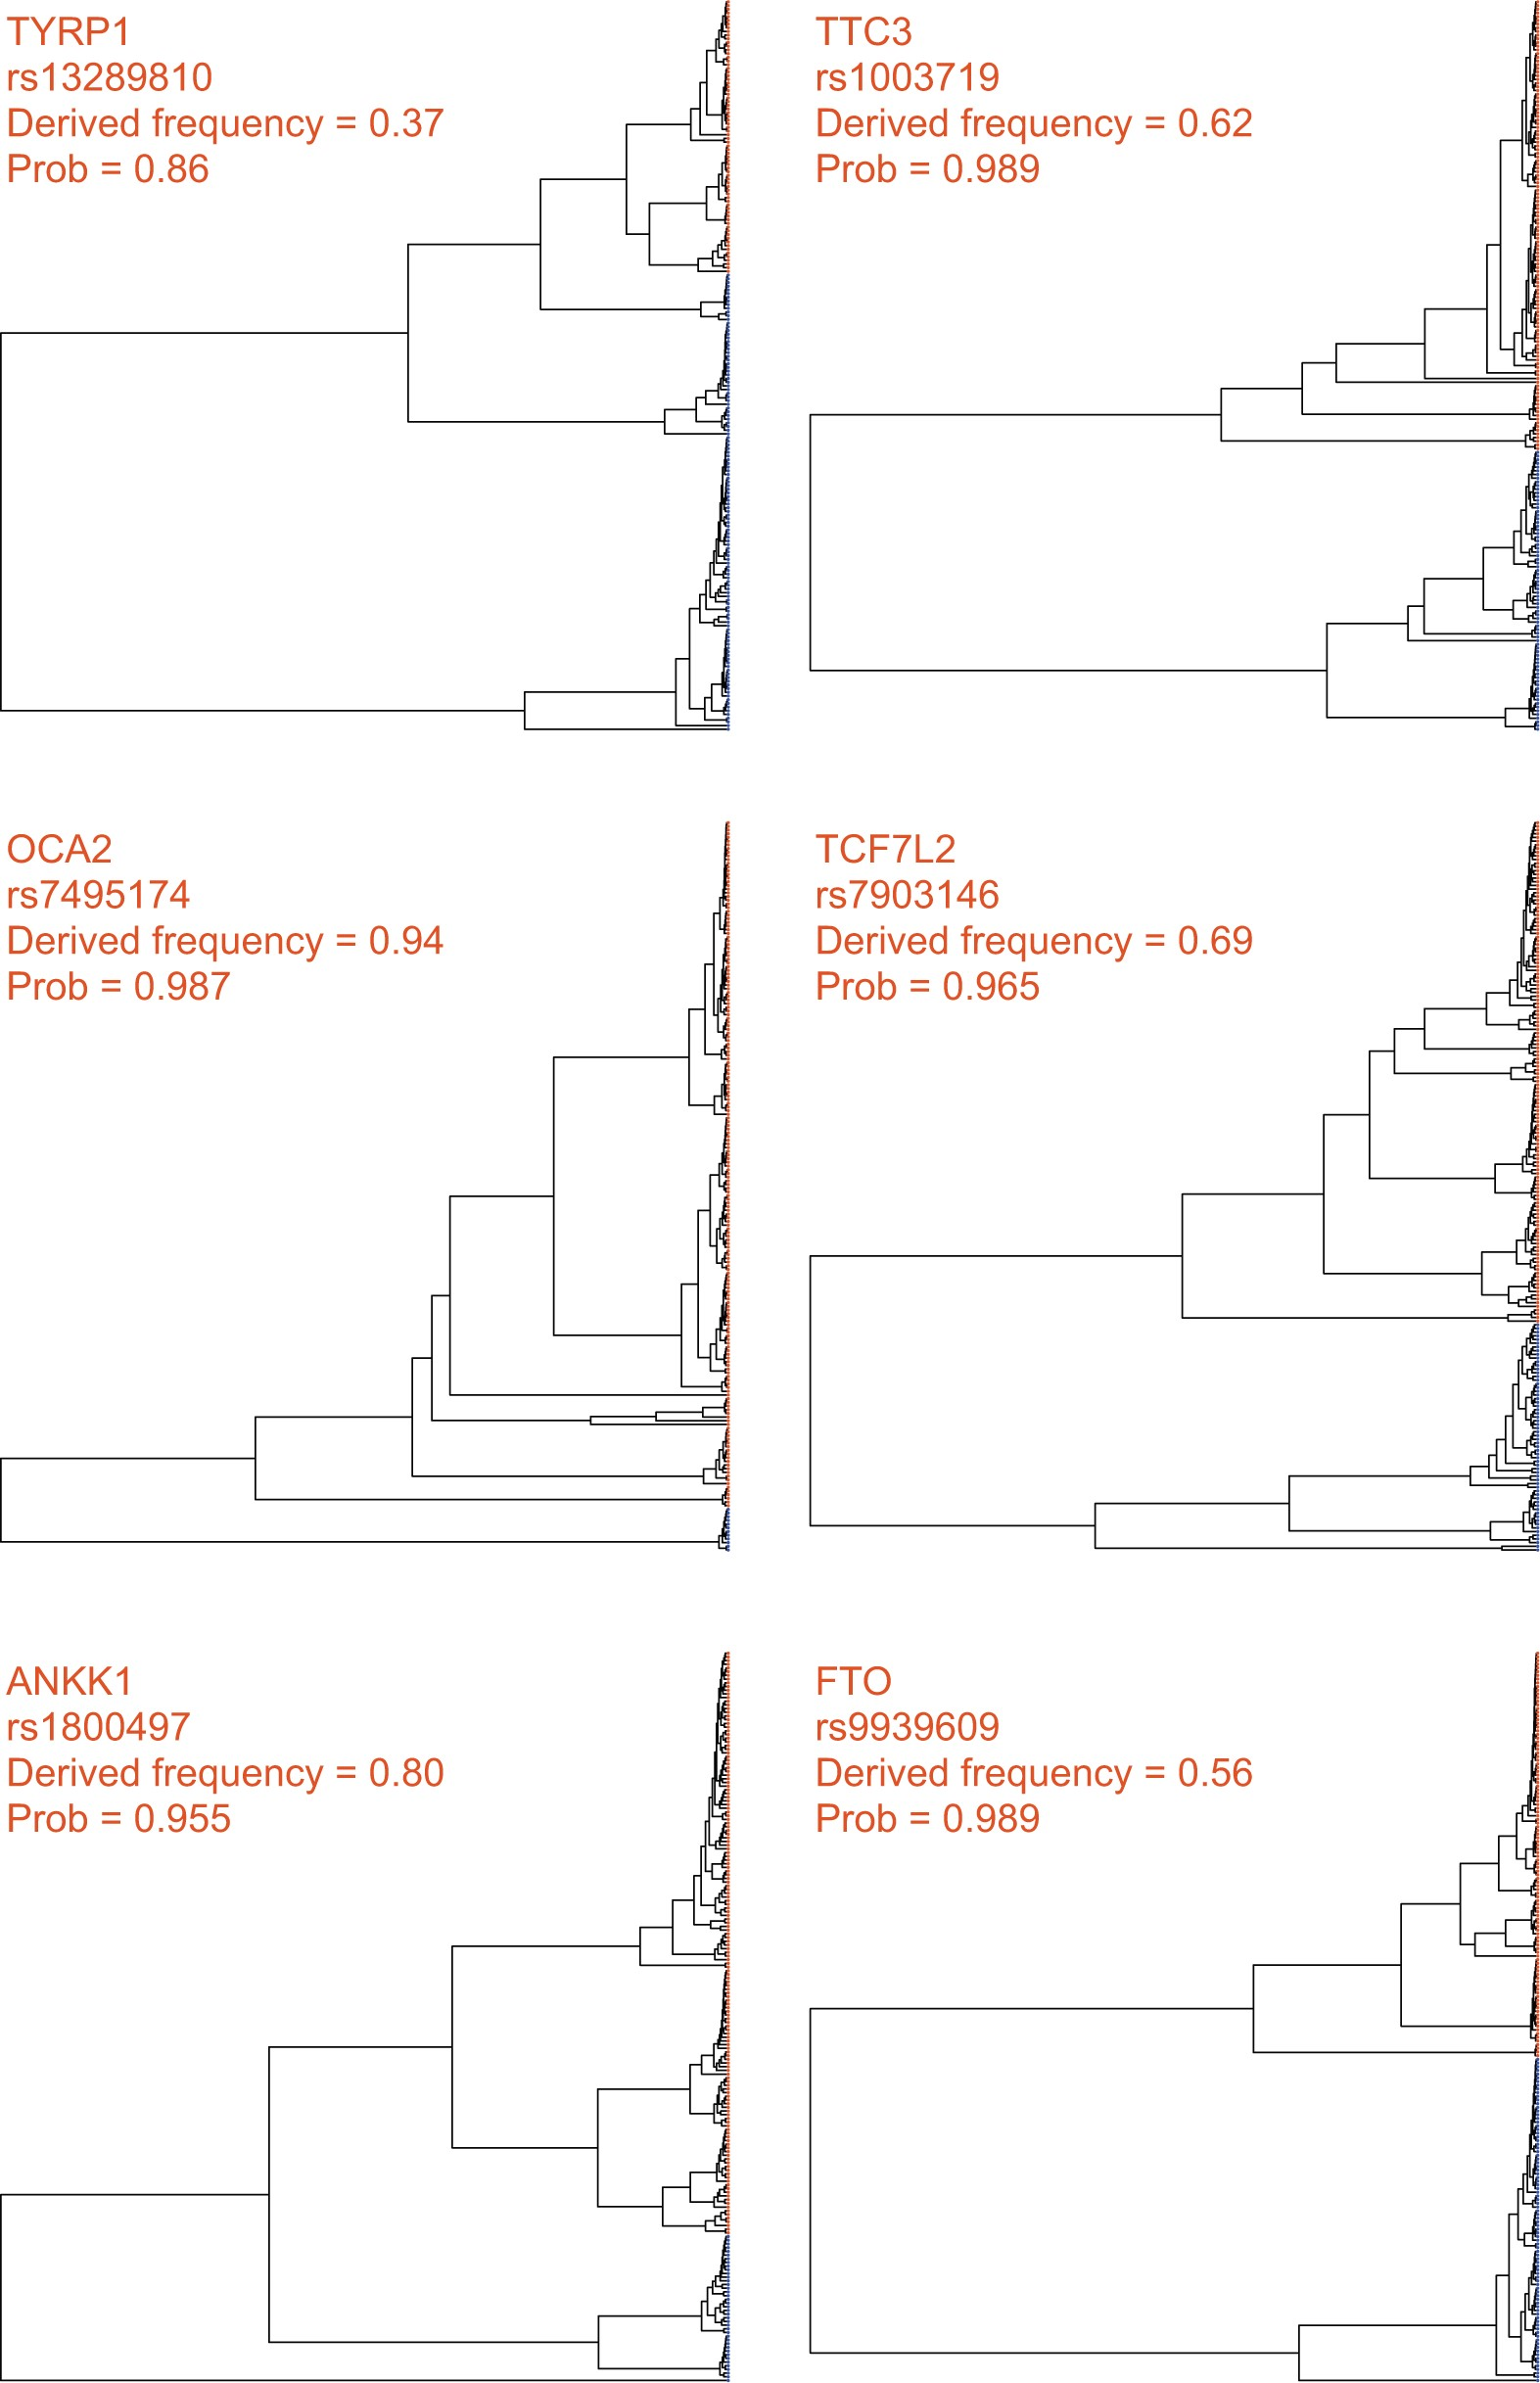
\includegraphics[scale=0.25]{SIA_figs/SIA_F6.jpeg}
    \caption[Local genealogies at six loci lacking signal of positive selection in the 1000 Genomes CEU population.]{\textbf{Local genealogies at six loci lacking signal of positive selection in the 1000 Genomes CEU population.} Gene name, RefSNP number, derived AF and probability of neutrality inferred by \ac{SIA} for each locus are indicated at the top of each panel (see Table \ref{tab:SIA-T1} for more details). Taxa carrying the ancestral and derived alleles are colored in blue and orange, respectively.}
    \label{fig:SIA-F6}
\end{figure}

\subsection{Southern capuchino species analysis}
Our previous study of southern capuchino seedeaters made use of the full \ac{ARG} and \ac{ML} to detect and characterize selective sweeps, and suggested that soft sweeps are the dominant mode of adaptation in these species (see \nameref{methods} for more details). To further characterize the targets and strengths of positive selection in these species, we applied \ac{SIA} to polymorphism data (\cite{turbek_rapid_2021}) for \textit{S. hypoxantha}, and adopted a conservative approach by reporting only sites with \ac{DAF} $\geq 0.5$, \ac{SIA}-inferred $s \geq 0.0025$, and \ac{SIA}-inferred sweep probability $P_{\mathrm{sweep}} \geq 0.99$ (see \nameref{methods}). In addition to loci near top $F_{\mathrm{ST}}$ peaks and known pigmentation-related genes (Table \ref{tab:SIA-T2}), we identified many more sites under positive selection located outside the previously scanned $F_{\mathrm{ST}}$ peaks, amounting to a total of 15,551 putative partial soft sweep sites across the 333 scanned scaffolds for \textit{S. hypoxantha}. These sites can be prioritized for further evaluation and downstream analysis. Notably, \ac{SIA} enabled us to distinguish between selection at regulatory and coding sequences, and we found that sweep loci near $F_{\mathrm{ST}}$ peaks and pigmentation genes fall mostly in noncoding regions (Table \ref{tab:SIA-T2}). We additionally surveyed all putative sweep sites identified by \ac{SIA} and found that they are indeed enriched in noncoding regions (Fisher’s exact test, $P = 6.80 \times 10^{-5}$), particularly noticeable in the “near-coding” regions (Fig. \href{https://academic.oup.com/mbe/article/39/1/msab332/6433161?login=true#supplementary-data}{S22 online}). Consistent with the observation that the most highly differentiated \acsp{SNP} among taxa are noncoding (\cite{campagna_repeated_2017,turbek_rapid_2021}), our finding suggests that positive selection may act on \textit{cis}-regulatory regions to drive differentiation and the subsequent speciation process. Furthermore, we examined many individual predictions in detail, considering the local trees inferred by Relate at these high-confidence predictions (Fig. \ref{fig:SIA-F7}). We found, in numerous cases, that these sweeps had distinct genealogical features, displaying evidence of a burst of coalescence events, corresponding to unusually large and young clades. Prominent examples include predictions near pigmentation-related genes \textit{ASIP}, \textit{KITL}, \textit{SLC45A2}, and \textit{TYRP1}.

\begin{table}
    \centering
    \caption{The top 25 $F_{\mathrm{ST}}$ peaks identified in \cite{hejase_genomic_2020} along with the number of partial soft sites in \textit{S. hypoxantha} identified for each scaffold using \ac{SIA}.}
    \vspace{5mm}
    \begin{tabular}{p{0.12\textwidth}p{0.22\textwidth}p{0.2\textwidth}p{0.12\textwidth}p{0.2\textwidth}}
        \hline
        \rowcolor{white} \textbf{Scaffold} & \textbf{Start position (Mb)} & \textbf{End position (Mb)} & \textbf{Length (kb)} & \textbf{No. of partial soft sites*} \\
        \hline
        59 & 5.74 & 5.86 & 120 & 11 \\
        118 & 7.16 & 7.22 & 60 & 5 \\
        252 & 0.40 & 0.54 & 140 & 3 \\
        257.1 & 21.24 & 21.78 & 540 & 26 \\
        257.2 & 24.40 & 24.84 & 440 & 43 \\
        257.3 & 28.66 & 28.96 & 300 & 10 \\
        257.4 & 31.30 & 31.38 & 80 & 8 \\
        257.5 & 5.78 & 6.20 & 420 & 25 (1) \\
        263 & 0.00 & 0.58 & 580 & 31 \\
        308 & 0.04 & 0.20 & 160 & 0 \\
        404.1 & 5.04 & 5.84 & 800 & 115 (7) \\
        404.2 & 10.76 & 10.96 & 200 & 30 \\
        412 & 3.38 & 3.62 & 240 & 15 \\
        430 & 10.98 & 11.10 & 120 & 24 \\
        567 & 2.50 & 2.80 & 300 & 0 \\
        637.1 & 6.00 & 6.32 & 320 & 2 \\
        637.2 & 6.84 & 6.92 & 80 & 4 \\
        762 & 1.65 & 1.73 & 80 & 30 \\
        766 & 1.98 & 2.10 & 120 & 1 \\
        791 & 9.90 & 9.98 & 80 & 15 \\
        1,717 & 0.92 & 0.98 & 60 & 7 \\
        3,622 & 0.96 & 1.36 & 400 & 8 \\
        1,635 & 3.71 & 3.75 & 40 & 4 \\
        1,954 & 2.8 & 2.9 & 100 & 17 \\
        579 & 0.1 & 0.16 & 60 & 0 \\
        \hline
        \rowcolor{white} \multicolumn{5}{p{0.95\textwidth}}{\textbf{Note}: To avoid cases with limited power, we focused on sites with segregating frequency $\geq 0.5$, \ac{SIA}-inferred $s > 0.0025$, and \ac{SIA}-inferred sweep probability $P_{\mathrm{sweep}} \geq 0.99$.} \\
        \rowcolor{white} \multicolumn{5}{p{0.95\textwidth}}{* The number of sweep sites in coding regions is shown in parenthesis.}
    \end{tabular}
    \label{tab:SIA-T2}
\end{table}

\begin{figure}
    \centering
    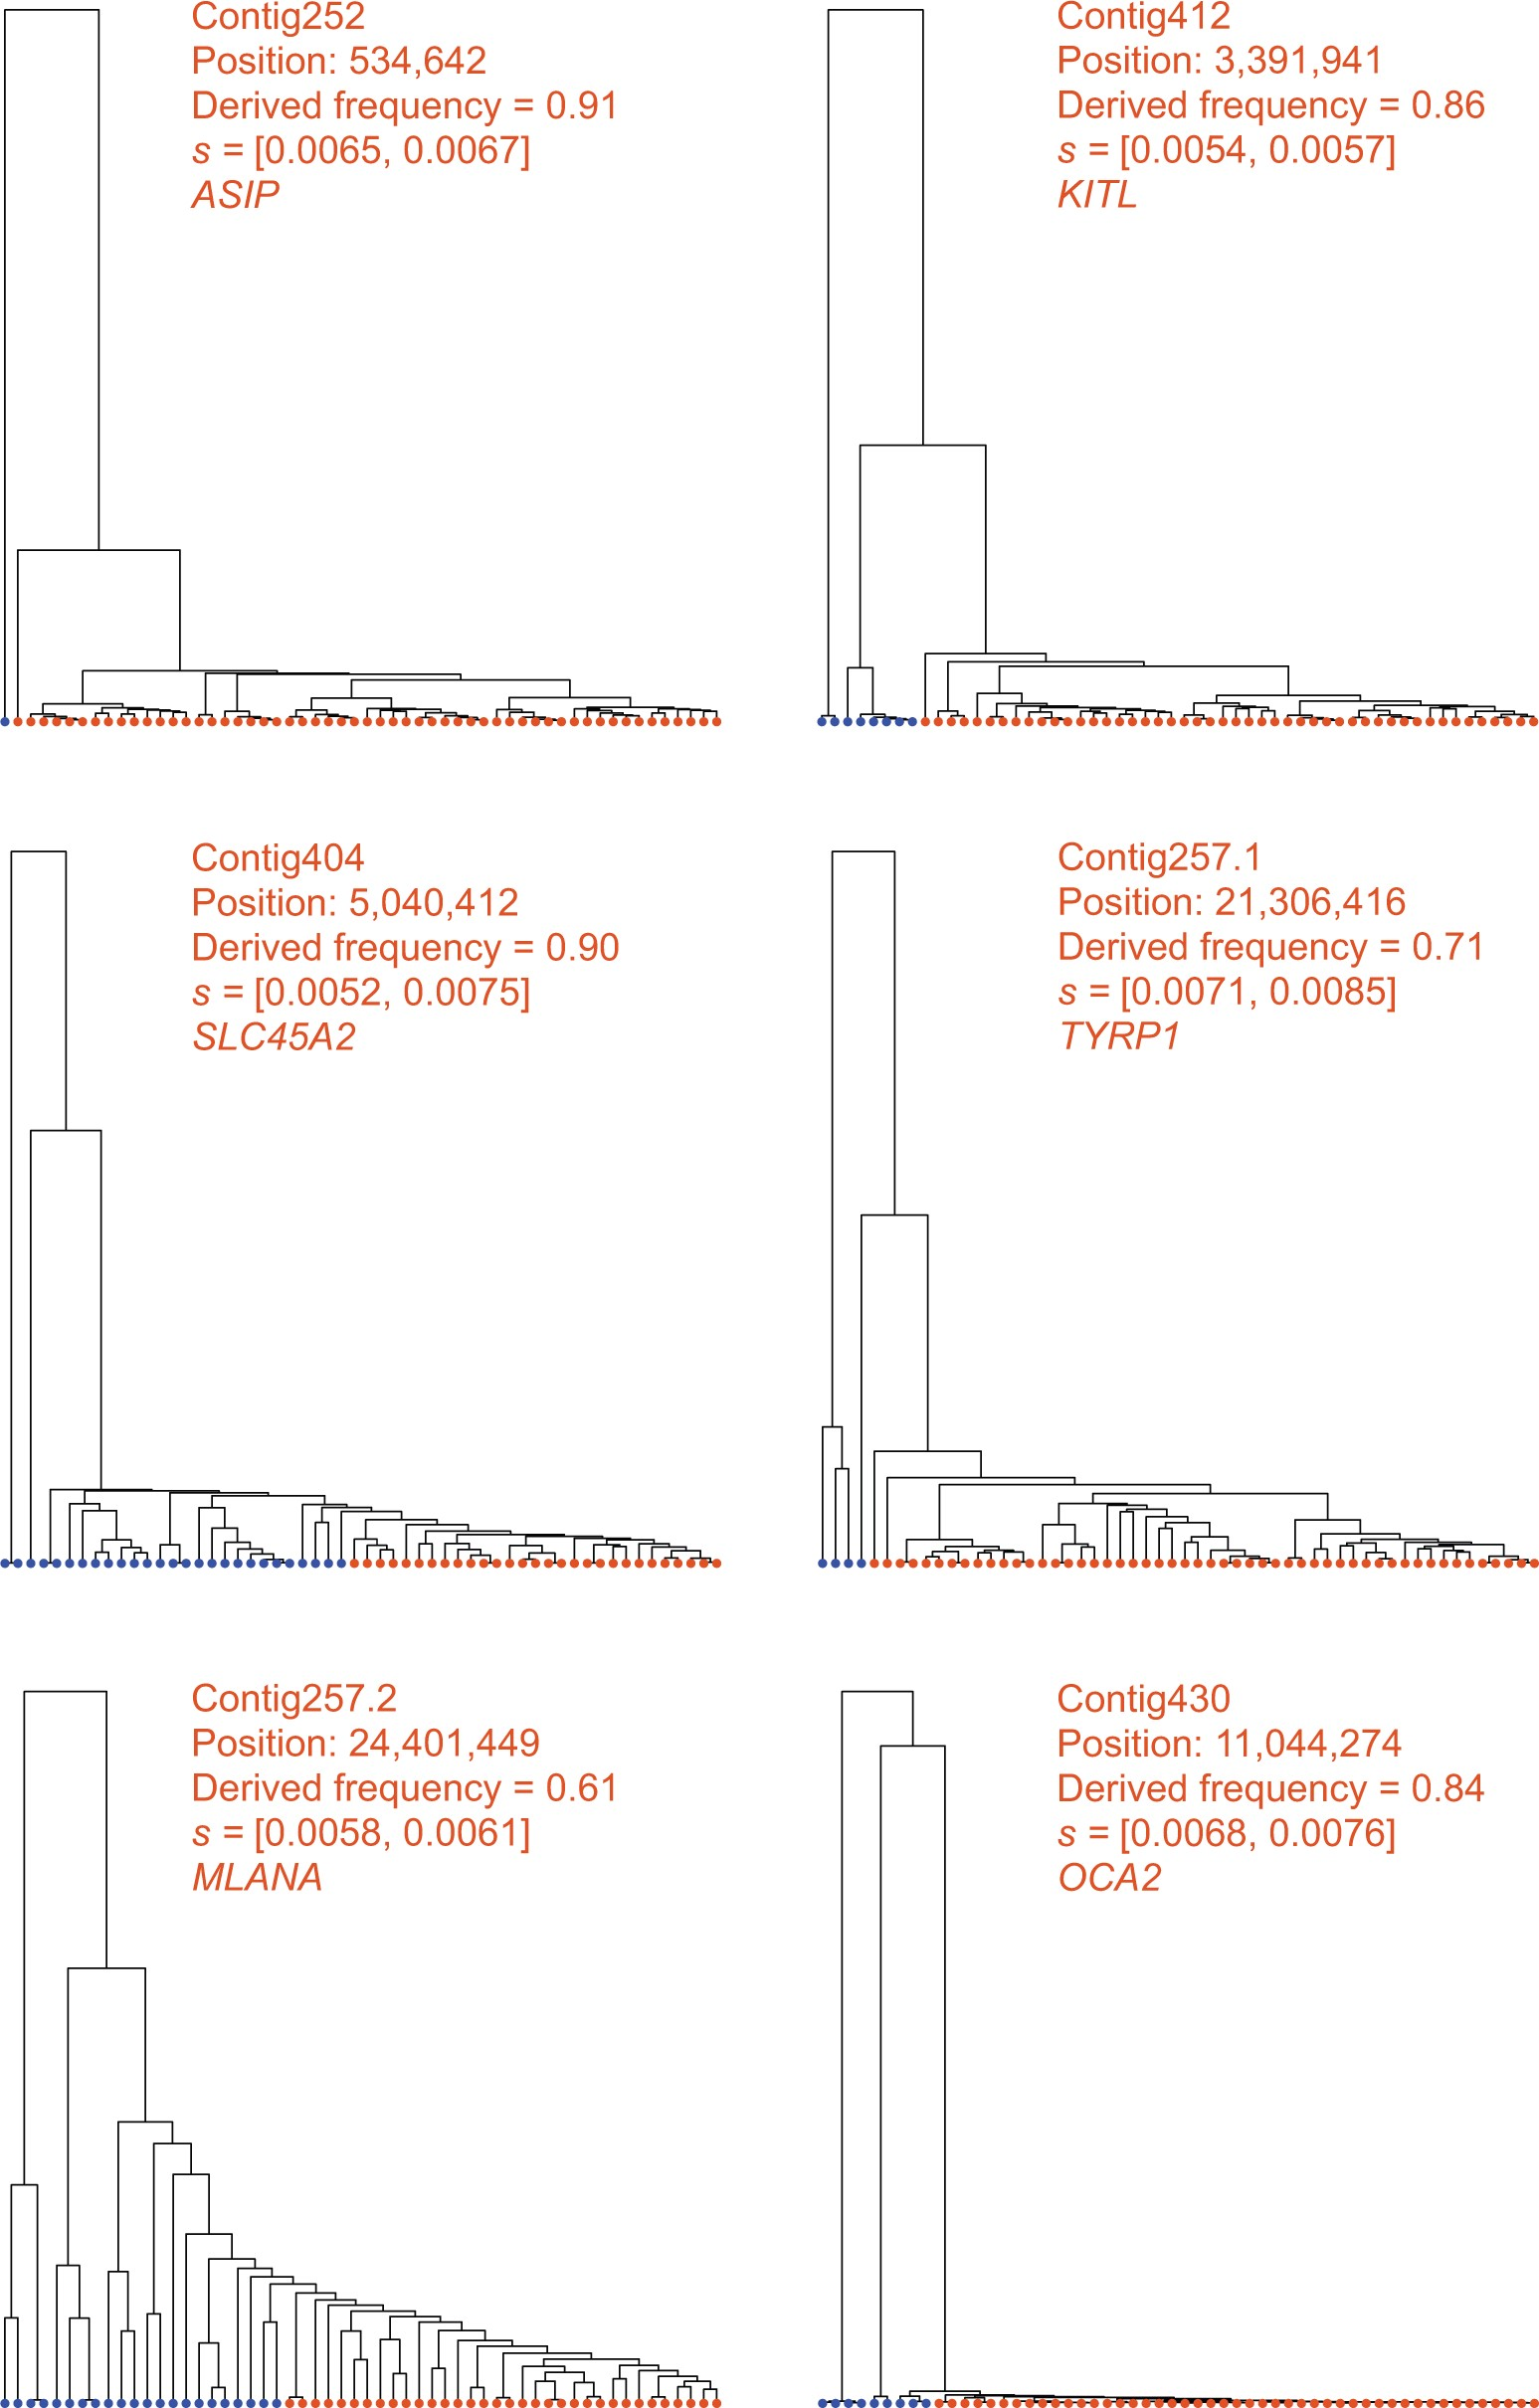
\includegraphics[scale=0.25]{SIA_figs/SIA_F7.jpeg}
    \caption[Local genealogies at six loci inferred to be under positive selection in \textit{S. hypoxantha}.]{\textbf{Local genealogies at six loci inferred to be under positive selection in \textit{S. hypoxantha}.} Contig name, position of \acs{SNP}, \ac{DAF}, \ac{SIA}-inferred selection coefficient range, and the pigmentation gene closest to the locus in question are indicated at the top of each panel. Haploid genomes carrying the ancestral and derived alleles are colored in blue and orange, respectively.}
    \label{fig:SIA-F7}
\end{figure}

\section{Discussion} \label{discussion}
The \ac{ARG} is useful for addressing a wide variety of biological questions ranging from inferring demographic parameters to estimating allele ages. \ac{SIA} exploits the particular utility of the \ac{ARG} for accurate inference of positive selection in a way that makes use of the full data set, as opposed to traditional summary statistics, which necessarily discard substantial information. Direct use of the \ac{ARG} improves upon traditional summary statistics in two key ways. First, it enables consideration of the temporal distribution of coalescence and recombination events in the history of the analyzed sequences, in contrast to traditional summary statistics that simply average over these coalescence and/or recombination events. In addition, \ac{ARG}-based methods provide better spatial resolution by separately examining individual genealogies and the recombination breakpoints between them, rather than averaging across windows containing unknown numbers of genealogies. These detailed patterns of coalescences and linkage enable the \ac{ARG}-based approaches to capture a more localized and fine-grained picture of selection (e.g., infer selection coefficient and \ac{AF} trajectory) as well as to achieve a better classification performance. This performance advantage is particularly noticeable at lower \acp{DAF} and when selection is weak, a regime where previous methods for selection inference fall short (Fig. \ref{fig:SIA-F2}).

At the same time, the supervised \ac{ML} approach sets \ac{SIA} apart from another \ac{ARG}-based method, CLUES, which approximates a full likelihood function for \acp{ARG} in the presence of selection using importance sampling and an \ac{HMM}. Although the accuracy of both \ac{SIA} and CLUES degraded when using inferred genealogies compared with true genealogies, reflecting the error and uncertainty at the \ac{ARG} inference step, \ac{SIA} appeared to be more robust to gene tree uncertainty (Figs. \ref{fig:SIA-F3} and \ref{fig:SIA-F4}). One possible reason for this observation is that CLUES effectively assumes that the selection coefficient at the focal site is conditionally independent of the flanking trees given the focal tree. This assumption should hold in the presence of fully specified genealogies, but it may make CLUES more sensitive to errors in the inferred genealogies. In other words, through its use of supervised learning, \ac{SIA} may be able to compensate for the effects of genealogy inference error on its estimation of the selection coefficient by also directly considering the flanking trees and \acs{LD}-related patterns among them. Still, the drop in accuracy observed across methods underscores the dependency of \ac{ARG}-based approaches on the \ac{ARG} inference method. For this reason, we anticipate that \ac{SIA} may benefit substantially from further improvement in \ac{ARG} inference tools (see \cite{hejase_summary_2020}).

The \ac{ARG}-based feature set distinguishes \ac{SIA} from other supervised \ac{ML} approaches for characterizing selective sweeps. \ac{SIA} uses local topological features of the \ac{ARG}, which are more informative than the \ac{SFS}- or \acs{LD}-based summary statistics employed by \ac{ML} methods such as S/HIC, SFselect, and evolBoosting. Using simulations, we demonstrated that the \ac{SIA} classifier outperformed a deep-learning method that aggregates these traditional summary statistics (Fig. \ref{fig:SIA-F2}). We also compared \ac{SIA} with ImaGene, which represents another flavor of supervised learning methods, inspired by the recent rise of \acp{CNN} for image recognition. ImaGene encodes sequence alignments as images for powerful population genetic inferences with \acp{CNN} and provides a state-of-the-art benchmark to compare against. We found that ImaGene performs remarkably well across a wide range of simulations, but \ac{SIA} does appear to be somewhat less biased and more robust to model mis-specification than ImaGene. The evolutionary information in the \ac{ARG} is implicit in the sequence alignment but some of this information may be difficult for a brute-force \ac{ML} model to discover directly.

We demonstrated that utilizing the \ac{ARG} granted \ac{SIA} considerably improved performance over deep-learning models solely employing traditional summary statistics. However, a possible drawback of an \ac{ARG}-based model is the potentially prohibitive computational overhead incurred by \ac{ARG} inference, especially as sample size grows. Picking a sample size when running \ac{SIA} involves a tradeoff between scalability (fewer samples, faster \ac{ARG} inference) and performance (more samples, slower \ac{ARG} inference). We have found that \ac{SIA} can infer selection coefficients reasonably well with as few as 16 haplotypes. Including more samples did improve performance but with a sublinear reduction in error (Fig. \href{https://academic.oup.com/mbe/article/39/1/msab332/6433161?login=true#supplementary-data}{S7 online}). Therefore, a sample size from a few dozen to a few hundreds—well within the capabilities of most modern \ac{ARG} inference methods—strikes a good balance between performance and scalability. Moreover, we found that larger sample sizes improved prediction performance primarily for alleles at lower frequencies but had little impact on the performance for more ancient alleles (as most lineages would have already coalesced going further back in time) (Fig. \href{https://academic.oup.com/mbe/article/39/1/msab332/6433161?login=true#supplementary-data}{S7 online}). This observation suggests that the choice of the sample size when applying \ac{SIA} should be guided by the biological question of interest -- ancient selection can be studied with just a handful of samples, whereas a larger sample size is better suited to detect more recent sweeps. Notably, the addition of ancient DNA samples could potentially enable selection to be inferred over much longer time scales. It should be possible to accommodate them with a relatively straightforward extension of the method.

Like other supervised learning methods, \ac{SIA} relies on simulations to generate training data. In order to apply \ac{SIA} in a particular population, a fresh set of training data tailored to that population needs to be simulated. Although it takes on the order of 100 CPU hours to simulate the training data compared with ten CPU hours to train the model (see \nameref{methods}), simulations can be easily distributed across multiple machines as each of them runs independently. Another potential drawback common to supervised methods is that they could be biased by subjective choices of simulation parameters. For example, \ac{SIA} and ImaGene cannot make accurate predictions of selection coefficients outside the range represented in the training data (Fig. \href{https://academic.oup.com/mbe/article/39/1/msab332/6433161?login=true#supplementary-data}{S20 online}), whereas unsupervised methods such as CLUES are not limited to a predefined range (Fig. \href{https://academic.oup.com/mbe/article/39/1/msab332/6433161?login=true#supplementary-data}{S21 online}). This problem could be circumvented by training on an extended range of $s$. Similarly, the tendency of \ac{SIA} to underestimate the selection coefficient for sites under weak selection (Figs. \ref{fig:SIA-F3} and \ref{fig:SIA-F4}) could be mitigated by augmenting the training set with simulations densely sampled from the weak selection regime. A more subtle issue, however, arises when the underlying generative process of the real data does not match the assumptions made for the simulations of the training data, potentially compromising the accuracy of the method when applied to real data. Thus, we tested \ac{SIA} on simulations with parameters mismatching those used in the training procedure. In general, we found that \ac{SIA} was fairly robust to alternative parameter values, although, as expected, performance did degrade somewhat under severely mis-specified models. Notably, \ac{SIA} achieved a similar level of robustness to model parameter mis-specification as the unsupervised (i.e., not relying on training data) likelihood method CLUES, yet outperformed the supervised deep-learning method ImaGene.

Applying \ac{SIA} to the CEU panel from the 1000 Genomes Project yielded several noteworthy findings at loci with known ties to phenotypes of interest. In addition to confirming the canonical signal of selective sweep at the \textit{LCT} locus, \ac{SIA} detected a novel signal of selection at a \acs{GWAS} \acs{SNP} in the \textit{MC1R} gene associated with red hair color, contrasting a previous study that could not find evidence of selection at \textit{MC1R} in the European population (\cite{harding_evidence_2000}). The derived allele at this locus segregates at around 10\% in the CEU population but is nearly absent in non-European populations (\cite{marcus_visualizing_2017}). In addition, at the \textit{MC1R} locus the Relate test statistic for selection (\cite{speidel_method_2019}), which tends to perform particularly well at low segregating frequencies (Fig. \ref{fig:SIA-F2}), falls slightly below the significance threshold of 0.05, supporting the evidence of positive selection at this locus. \ac{SIA} also detected evidence of selection at a \acs{SNP} in the \textit{ABCC11} gene reported to be the determinant of wet versus dry earwax as well as sweat production, mirroring the signal of selection previously found in the East Asian population (\cite{ohashi_impact_2011}), although selection in the CEU population appeared to be much weaker. In addition, \ac{SIA} identified selection at a few other pigmentation-related loci, yet determined previously identified \acsp{SNP} in the \textit{TYRP1} and \textit{TTC3} genes to be largely free from selection (Table \ref{tab:SIA-T1}). These results were consistent with a previous study (\cite{stern_approximate_2019}), which reported similar results for these pigmentation-related loci, albeit in a slightly different population (GBR). \ac{SIA} notably did not detect positive selection at \acs{GWAS} loci in the \textit{TCF7L2} gene associated with type-2 diabetes, the \textit{ANKK1} gene implicated in addictive behaviors, and the \textit{FTO} gene associated with obesity. Overall, this empirical study with the 1000 Genomes CEU population has illustrated how \ac{SIA} can be applied to assess natural selection at the resolution of individual sites, suggesting that it may be useful in prioritizing \acs{GWAS} variants for further scrutiny.

In our previous work on southern capuchino seedeaters (\cite{hejase_genomic_2020}) (see \nameref{methods}), we applied newly developed statistical methods for \ac{ARG} inference and \ac{ML} for the prediction of selective sweeps. We found evidence suggesting that a substantial fraction of soft sweeps is partial but had limited power to identify them (i.e., average accuracy of 56\%). \ac{SIA} considerably improved our characterization of positive selection in the southern capuchino species in two key ways. The \ac{SIA} framework performs inference of selection directly from genealogies instead of traditional summary statistics, and in doing so achieved an accuracy of up to 96\% in detecting partial soft sweeps. Consequently, we found abundant evidence of soft sweeps beyond the previously scanned $F_{\mathrm{ST}}$ peaks, and additionally were able to estimate their selection coefficients. Importantly, \ac{SIA} also took the analysis of selection beyond broad genomic windows containing sweeps to the identification of specific putative causal variants. We took advantage of this substantial improvement in genomic resolution and analyzed the distribution of these sweep sites, which revealed that positive selection on regions that likely contain \textit{cis}-regulatory elements plays a role in driving the differentiation and speciation of southern capuchino seedeaters.

Although we believe \ac{SIA} represents an important step forward in the use of the \ac{ARG} for \ac{ML}-based selection inference, there remain several possible avenues for improvement. For example, \ac{SIA} currently uses a point-estimate of the \ac{ARG}, rather than a distribution, and therefore does not explicitly take gene-tree uncertainty into account. Instead, the uncertainty of the inferred parameters is estimated with neural network dropouts (\cite{gal_dropout_2016}). The variance of parameter inference could alternatively be assessed from uncertainty in genealogy reconstruction by resampling coalescent times with Relate (\cite{speidel_method_2019}), and moreover resampling trees from the posterior distribution of \acp{ARG} with ARGweaver (\cite{rasmussen_genome-wide_2014}). Thus, it may be enlightening to compare these different approaches to analyzing uncertainty. Likewise, \ac{SIA} will greatly benefit from better algorithms for \ac{ARG} reconstruction that balance accuracy with scalability and can handle thousands of genomes. In addition, the \ac{SIA} framework was applied in the context of single-locus selective sweeps, but could be extended to study polygenic selection, by making use of summary statistics from genome-wide association studies (as in \cite{stern_disentangling_2021}) and adapting the architecture of our neural network to account for selection acting at multiple sites. Finally, the robustness of \ac{SIA} to model mis-specifications can be further improved by ensuring the simulated data is generated under a distribution that is compatible with the real target data set. We anticipate that the continual advancement in \ac{ARG} inference methods has the potential to open up many new applications for this flexible and powerful model of \ac{ARG}-based deep learning in population genetics.

\section{Materials and methods} \label{methods}

\subsection{Simulated data sets used for training and testing the \ac{SIA} model}
Training and testing data sets were generated using discoal (\cite{kern_discoal_2016}) by simulating 1,000,000 regions of length 100 kb for each model we considered (i.e., “neutral” or “hard sweep”). Aside from these regions, 2,000 were simulated for validation and 5,000 were simulated for testing. The number of sampled sequences was selected to match the number of individuals in the CEU population in the 1000 Genomes data set. Thus, a total of 198 haploid sequences were sampled. Simulations used a demographic model based on European demography (\cite{tennessen_evolution_2012}). In non-neutral simulations, selection was applied to a single focal site located in the middle of the simulated region. We sampled each of the main demographic and selection parameters from a uniform distribution: 1) mutation rate $\mu \sim \mathcal{U}(1.25\times 10^{-8}, 2.5\times 10^{-8})$; 2) recombination rate $\rho \sim \mathcal{U}(1.25\times 10^{-8}, 2.5\times 10^{-8})$; 3) selection coefficient $s \sim \mathcal{U}(0.0001, 0.02)$; and 4) segregating frequency of the site under selection $f \sim \mathcal{U}(0.01, 0.99)$. The total storage footprint for the simulations was 1.6TB. The average cost of one simulation was 0.53 s, amounting to a total of 148 CPU hours to simulate the entire training set. The cost of simulation was mitigated by parallelization across multiple compute nodes.

\subsection{ARG feature extraction} \label{fea-xtract}
For each target variant, we extracted the corresponding gene tree from the \ac{ARG}, then overlaid it with 100 discrete timepoints. These timepoints were fixed across all trees in an approximately log-uniform manner that resulted in finer discretization of more recent time scales (as in \cite{rasmussen_genome-wide_2014}). We considered biallelic sites only and assumed no recurrent mutations; thus, each mutation was assumed to occur on the branch of the tree where the ancestral allele switches to the derived. For each timepoint, we calculated the number of active ancestral and derived lineages. Furthermore, we computed the number of all active lineages (not distinguishing between ancestral and derived) at the same set of predefined timepoints in the two left- and right-flanking gene trees to account for linkage disequilibrium. We experimented with alternative numbers of flanking gene trees and found that the \ac{SIA} model with two flanking gene trees (\ac{RMSE} = 0.0027) outperforms a model with one (\ac{RMSE} = 0.0029) or no (\ac{RMSE} = 0.0030) flanking gene tree. Generally, more gene trees provide \ac{SIA} with richer linkage information and thus improve its ability to estimate the effect of positive selection on a locus. The exact threshold of diminishing returns, however, can be computationally costly to establish. We therefore opted to include two flanking gene trees while noting that the user can control this hyperparameter when running \ac{SIA}.

In the end, the \ac{ARG} feature for each locus consisted of a 600-dimensional vector, which was then used as input to an \ac{RNN}. The features for each simulated sweep region were extracted from the sweep site (by default at the center in all simulations) whereas the features for a simulated neutral region were extracted from a variant site (randomly chosen) with a predefined matched \ac{DAF}. The features for each genomic locus of interest in the CEU population were extracted from all variant sites at that locus having a \ac{DAF} of $>0.05$.

\subsection{Training \iac{RNN} to predict different modes of selection}
An \ac{RNN} was applied to the simulated training data sets to learn a classification or regression model for the task at hand. We used \iac{LSTM}, a particular form of \ac{RNN}, to accommodate the temporal nature of our features, account for long-term dependencies, and tackle the vanishing gradient problem observed in traditional \acp{RNN}. Our model had 100 timepoints with the final target output depending on the use of classification or regression. For the classification task, the final target output is a binary class label predicting whether a region is under selection or neutrality. For the regression task, the final target output is a continuous value, representing the selection coefficient or the time of selection onset. We also took a many-to-many approach to model the \ac{AF} trajectory for the site under selection. The \texttt{Keras} software was used to train and test the model. We used a two-stacked \ac{LSTM} to account for greater model complexity where the number of units in each stack was set to 100 and the hyperbolic tangent (\texttt{tanh}) was used as an activation function. The \texttt{Adam} optimization method with its default operating parameters was used to update the network weights. For the classification task, the \texttt{Softmax} activation function was applied on the final dense layer and the \texttt{binary\_crossentropy} was used to compute the cross-entropy loss between true labels and predicted labels. For the regression task, the \texttt{linear} activation function was applied on the final dense layer and the \texttt{mean\_squared\_error} loss was used. The \ac{SIA} deep-learning model took on average 7–10 h to train on a single \acs{GPU} node with 32 GB memory and four threads, whereas applying the trained model for prediction took less than a minute.

\subsection{Estimation of confidence intervals}
To turn our single-valued regression model into one capable of returning a distribution of predictions of $s$, we reused the dropout technique that is typically used during training. Dropout enables a fraction of nodes to be randomly “turned off” in a certain layer, which assists in the regularization of the model and helps prevent overfitting. We applied dropout during inference, enabling us to sample a “thinned” network to generate a sample prediction. By repeatedly sampling thinned networks, we generated a distribution of predictions and then computed confidence intervals based on this distribution (\cite{gal_dropout_2016}).

\subsection{\ac{ARG} inference}
Relate (\cite{speidel_method_2019}) (\texttt{v1.0.17}) was used for inferring \acp{ARG} underlying simulated genomic samples as well as the CEU population in the 1000 Genomes data set. For simulations under the \cite{tennessen_evolution_2012} demography, Relate was run with the true simulation parameters ($\mu$, $\rho$, and $N_e$) specified; whereas for genomic loci of the CEU population, Relate was run with a mutation rate of $2.5 \times 10^{-8}$/base/generation (\texttt{-m 2.5e-8}), a constant recombination map of $1.25 \times 10^{-8}$/base/generation and a diploid effective population size of 188,088 (\texttt{-N 376176}). The choice of mutation rate follows \cite{stern_approximate_2019} based on estimates from \cite{nachman_estimate_2000}. Although some more recent estimates have been lower (\cite{scally_revising_2012}), these differences in mutation rate are unlikely to have a major effect on our selection inference because \ac{SIA} appears to be fairly robust to mis-specification of mutation rate (Figs. \href{https://academic.oup.com/mbe/article/39/1/msab332/6433161?login=true#supplementary-data}{S13 and S16 online}). For simulations and genomic loci of the \textit{S. hypoxantha} population, Relate was run with $\mu = \rho = 1 \times 10^{-9}$/base/generation and a diploid $N_e$ of 130,000. The branch lengths of Relate-inferred genealogies were estimated iteratively with the \texttt{EstimatePopulationSize.sh} script in the Relate package. Specifically, population size history was inferred from the \ac{ARG}, the branch lengths are then updated for the estimated population size history and these steps are repeated until convergence. This was done for a default of five iterations (\texttt{-num\_iter 5}).

\subsection{Alternative methods for selection inference}
To benchmark the performance of \ac{SIA} for classification of sites under neutrality versus selective sweep, we ran the following methods: Tajima’s $D$ (\cite{tajima_statistical_1989}), H1 (\cite{garud_recent_2015}), iHS (\cite{voight_map_2006}), a summary statistics-based deep-learning model, and a tree-based statistic that is part of the Relate (\cite{speidel_method_2019}) program. Tajima’s $D$, H1, and iHS were calculated with the \texttt{scikit-allel} package. Haplotypes of the entire 100 kb simulated genomic segment were used for Tajima’s $D$ and H1 calculations. The unstandardized iHS was computed at every site with minor \ac{AF} $>5\%$, with respect to all other sites in the genomic segment (\texttt{min\_maf = 0.05, include\_edges = True}). iHS scores of all sites were then standardized in 50 \ac{AF} bins. Finally, the iHS score of a genomic region was taken to be the mean of the iHS scores of all of its variant sites. For the summary statistics-based deep-learning model, we made use of the summary statistics used by S/HIC (\cite{schrider_shic_2016,kern_diploshic_2018}) as features for our deep-learning architecture. These included 11 sequence-based summary statistics (see Figure 3 in \cite{schrider_supervised_2018}) which were used as features for our deep-learning model to distinguish among the two classes at hand (selective sweep vs. neutral drift). All statistics were collected along five consecutive 20-kb windows with the objective of identifying possible sweeps induced by a positively selected mutation in the third (middle) window. Some of these summary statistics corresponded to standard measures of diversity, such as ss (the number of segregating sites), $\pi$ (\cite{nei_mathematical_1979}), Tajima’s $D$ (\cite{tajima_statistical_1989}), $\theta_{\mathrm{W}}$ (\cite{watterson_number_1975}), $\theta_{\mathrm{H}}$ (\cite{fay_hitchhiking_2000}), the number of distinct haplotypes (\cite{messer_population_2013}), H1, H12, H2/H1 (\cite{garud_recent_2015}), $Z_{\mathrm{nS}}$ (\cite{kelly_test_1997}), and maximum value of $\omega$ (\cite{kim_linkage_2004}). For each of these statistics, we computed an average value for each of the five 20 kb windows for the simulated population. Finally, each summary statistic was normalized by dividing the value recorded for a given window by the sum of values across all five windows. The Relate tree-based selection test was performed with an add-on module (\texttt{DetectSelection.sh}) using the inferred genealogy with calibrated branch lengths at a site of interest, yielding a $\log_{10}P$ value for each site.

We also compared the performance of \ac{SIA} for selection coefficient inference with that of CLUES (\cite{stern_approximate_2019}) and a genotype-based \ac{CNN} framework (\cite{flagel_unreasonable_2019,torada_imagene_2019}). Selection coefficient inference from true genealogies was performed with \texttt{clues-v0} (\href{https://github.com/35ajstern/clues-v0}{last accessed November 28, 2021}). Transition probability matrices were built on a range of selection coefficients $[0, 0.05]$ at increments of 0.0001 and present-day allele frequencies $[0.01, 0.99]$ at increments of 0.01. Selection coefficient inference from Relate inferred genealogies was performed with CLUES (\href{https://github.com/35ajstern/clues}{last accessed November 28, 2021}). Branch lengths of the genealogy at the site of interest were resampled with Relate for 600 \acs{MCMC} iterations, and CLUES was run with the following arguments: \texttt{-tCutoff 10000 -burnin 100 -thin 5}. For the genotype-based \ac{CNN} model, each simulated genomic segment was preprocessed by first sorting the haplotypes and then converting the segment to a fixed-size genotype matrix. Haplotype sorting was performed by 1) calculating the pairwise Manhattan distances between haplotypes; 2) setting the haplotype with the smallest total distance to all other haplotypes as the first haplotype; and 3) sorting the remaining haplotypes in increasing distance to the first haplotype. To convert the sorted haplotypes to a fixed-size genotype matrix, centered on the middle variant of a simulated region, up to 180 variants on each side were retained. Variants beyond 180 were discarded and if there were fewer than 180, the missing variants were padded with zeros. Ancestral and derived alleles were coded with 0s and 1s, respectively. Consequently, each simulated genomic region was encoded as a $(198 \times 360)$ binary matrix, along with a real-valued vector encoding the genomic positions of the variants in the matrix. The \ac{CNN} model had a branched architecture -- one branch with five 1D convolution layers taking the genotype matrix as input and another branch with a fully connected layer taking the vector of variant positions as input. The output of the two branches was flattened, concatenated and fed into three fully connected layers, followed by a linear output layer to predict selection coefficient (Fig. \href{https://academic.oup.com/mbe/article/39/1/msab332/6433161?login=true#supplementary-data}{S23 online}).

\subsection{Evaluation metrics}
To evaluate the performance of \ac{SIA}’s classification model and alternative methods, we computed an \ac{ROC} curve for the binary class at hand (“neutral” or “sweep”), to provide a more complete summary of the behavior of different types of errors. We further assessed the performance of \ac{SIA} and alternative methods in terms of correctly predicting the selection coefficient numerically using \acf{MAE}, \acf{RMSE}, coefficient of determination ($r^2$), and visually using a box plot that compares the simulated ground truth against the predictions by the method at hand.

\subsection{Robustness study}
We carried out an extensive analysis of the robustness of our approach, considering not only alternative demographic parameters (such as population size), but also alternative parameters for recombination rate, mutation rate, time of selection onset, and selection coefficients. In all cases, we took care to test our prediction methods under parameters well outside the range used in training.

\subsection{Analysis of CEU population in 1000 Genomes data}
We applied \ac{SIA} to infer selection coefficients and \ac{AF} trajectories in the 1000 Genomes (\cite{auton_global_2015}) CEU population at 13 genomic loci with known association to phenotypes, some of which were previously identified as likely targets of positive selection (Table \ref{tab:SIA-T1}). For each gene of interest, the \ac{ARG} was inferred with Relate from \acsp{SNP} within a 2-Mb window centered at the gene. Once the \ac{ARG} was inferred, only \acsp{SNP} with valid ancestral allele (``\texttt{AA}" \texttt{INFO} field in the \texttt{vcf} file) were retained for downstream analysis. Following the aforementioned protocol (see \nameref{fea-xtract}), features at all variant sites in the 2 Mb window above \iac{DAF} threshold of 0.05 were extracted. Lastly, the \ac{SIA} model was applied to classify neutrality versus selection, and infer selection coefficient and \ac{AF} trajectory at each site.

\subsection{Localizing sweeps in southern capuchino seedeaters}
We recently applied a combination of \ac{ARG} inference and \ac{ML} methods for identifying selective sweeps to study previously identified “islands of differentiation” in southern capuchino seedeaters and distinguish among possible evolutionary scenarios leading to their formation (\cite{hejase_genomic_2020}). Taking advantage of its improved power and genomic resolution, we applied \ac{SIA} to sequence data for the species for which we have the most samples, \textit{S.hypoxantha}. We simulated training (250,000 neutral; 250,000 soft sweeps), validation (1000 neutral; 1000 soft sweeps), and testing (2,500 neutral; 2,500 soft sweeps) data sets for \ac{SIA} under a demographic model inferred by G-PhoCS (\cite{campagna_distinguishing_2015}). Simulations were performed using discoal with the following parameters: 1) mutation rate $\mu = 1\times 10^{-9}$; 2) recombination rate $\rho = 1\times 10^{-9}$; 3) derived $N_e = 130,000$; 4) root divergence time = 1,850,000 generations ago; 5) root $N_e = 1,450,000$; 6) ancestral divergence time = 44,000 generations ago; 7) ancestral $N_e = 14,380,000$; 8) selection coefficient $s \sim \mathcal{U}(0.001, 0.02)$; 9) initial frequency at which selection starts acting on the allele $f_{\mathrm{init}} \sim \mathcal{U}(0.01, 0.05)$; and 10) segregating frequency of the site under selection $f \sim \mathcal{U}(0.25, 0.99)$. A total of 56 haploid sequences were sampled from each simulation, matching the number of \textit{S. hypoxantha} individuals (28) in the real data. The \ac{SIA} model for \textit{S. hypoxantha} was built, trained and evaluated in an otherwise similar fashion to that for the CEU population as outlined above.

Using a subset of polymorphism data from \cite{turbek_rapid_2021} of 28 \textit{S. hypoxantha} and 2 \textit{S. minuta} individuals, we applied our trained model to localize selective sweeps in \textit{S. hypoxantha} on 19 scaffolds that contain top $F_{\mathrm{ST}}$ peaks in at least one pairwise species comparison (\cite{campagna_repeated_2017}) and/or harbor known pigmentation-related genes such as \textit{ASIP} (located on scaffold 252; induces melanocytes to synthesize pheomelanin instead of eumelanin), \textit{KITL} (located on scaffold 412; stimulates melanocyte proliferation), \textit{SLC45A2} (located on scaffold 404; transports substances needed for melanin synthesis), and \textit{CAMK2D} (located on scaffold 1717; cell communication), as well as 316 scaffolds that 1) are longer than 100 kb; 2) contain more than 1,000 variants; and 3) where more than 95\% of sites have a consensus ancestral allele, as determined by four identical haplotypes for two individuals from the outgroup species \textit{S. minuta}. The \ac{ARG} was inferred with Relate for each scaffold independently. Once the \ac{ARG} was inferred, the \ac{SIA} model was applied to sites with consensus ancestral allele for classification and selection coefficient inference.

\section{Supplementary material}

Supplementary figures are available at \href{https://academic.oup.com/mbe/article/39/1/msab332/6433161#supplementary-data}{\textit{Molecular Biology and Evolution} online}. The simulation scripts and code for building and training the \ac{SIA} model are publicly available on \href{https://github.com/CshlSiepelLab/arg-selection}{GitHub}.
\chapter{Selective sweeps on different pigmentation genes mediate convergent evolution of island melanism in two incipient bird species}

\textit{Content of this chapter was published in PLoS Genetics (2022) under the title "Selective sweeps on different pigmentation genes mediate convergent evolution of island melanism in two incipient bird species" by Leonardo Campagna, Ziyi Mo, Adam Siepel and J. Albert C. Uy. L.C. conceptualized the study, curated data, performed formal analyses, developed methodology and wrote the manuscript. Z.M. characterized selective sweeps in the bird populations using the SIA method, developed methodology and edited the manuscript. A.S. developed methodology and edited the manuscript. J.A.C.U. conceptualized the study, curated data, performed formal analyses, developed methodology and wrote the manuscript.}

\section{Part 1}
blabla
\chapter{Domain-adaptive neural networks improve supervised machine learning based on simulated population genetic data} \label{chapter4}

\textit{Content of this chapter was previously uploaded to bioRxiv (2023) under the title ``Domain-adaptive neural networks improve supervised machine learning based on simulated population genetic data" by Ziyi Mo and Adam Siepel. The manuscript was published in PLoS Genetics (2023) under the same title.}

\section{Abstract}
Investigators have recently introduced powerful methods for population genetic inference that rely on supervised machine learning from simulated data. Despite their performance advantages, these methods can fail when the simulated training data does not adequately resemble data from the real world. Here, we show that this “simulation mis-specification” problem can be framed as a “domain adaptation” problem, where a model learned from one data distribution is applied to a dataset drawn from a different distribution. By applying an established domain-adaptation technique based on \iac{GRL}, originally introduced for image classification, we show that the effects of simulation mis-specification can be substantially mitigated. We focus our analysis on two state-of-the-art deep-learning population genetic methods—\ac{SIA}, which infers positive selection from features of the \acf{ARG}, and ReLERNN, which infers recombination rates from genotype matrices. In the case of \ac{SIA}, the domain adaptive framework also compensates for \ac{ARG} inference error. Using the \ac{dadaSIA} model, we estimate improved selection coefficients at selected loci in the 1000 Genomes CEU population. We anticipate that domain adaptation will prove to be widely applicable in the growing use of supervised machine learning in population genetics.

\section{Introduction}
Advances in genome sequencing have allowed population genetic analyses to be applied to many thousands of individual genome sequences (\cite{auton_global_2015,sudlow_uk_2015,karczewski_mutational_2020}). Given adequately rigorous and scalable computational tools for analysis, these rich catalogs of genetic variation provide opportunities for addressing many important questions in areas such as human evolution, plant genetics, and the ecology of non-model organisms. Deep-learning methods, already well-established in other application areas (\cite{lecun_deep_2015}), have proven to be good matches for these analytical tasks and have recently been successfully applied to many problems in population genetics (\cite{sheehan_deep_2016,kern_diploshic_2018,schrider_supervised_2018,flagel_unreasonable_2019,torada_imagene_2019,adrion_predicting_2020,caldas_inference_2022,hejase_deep-learning_2022,korfmann_deep_2023,huang_harnessing_2023}).

The key to the success of deep learning in population genetics has been the use of large amounts of simulated data for training. Under simplifying, yet largely realistic, assumptions, evolution plays by relatively straightforward rules. By exploiting these rules and advances in computing power, a new generation of computational simulators has made it possible to efficiently produce large quantities of perfectly labeled synthetic data across a wide range of evolutionary scenarios (\cite{haller_tree-sequence_2019,haller_slim_2019,baumdicker_efficient_2022}). At the same time, programming libraries such as stdpopsim have made these simulators accessible to a broad community of researchers while improving the reproducibility of simulation workflows (\cite{adrion_community-maintained_2020,lauterbur_expanding_2022}). The facility of generating synthetic training data serves as the foundation of the new simulate-and-train paradigm of supervised machine learning for population genetics inference (Fig. \ref{fig:DA-F1}A; \cite{schrider_supervised_2018,korfmann_deep_2023,huang_harnessing_2023}).

\begin{figure}[h]
    \centering
    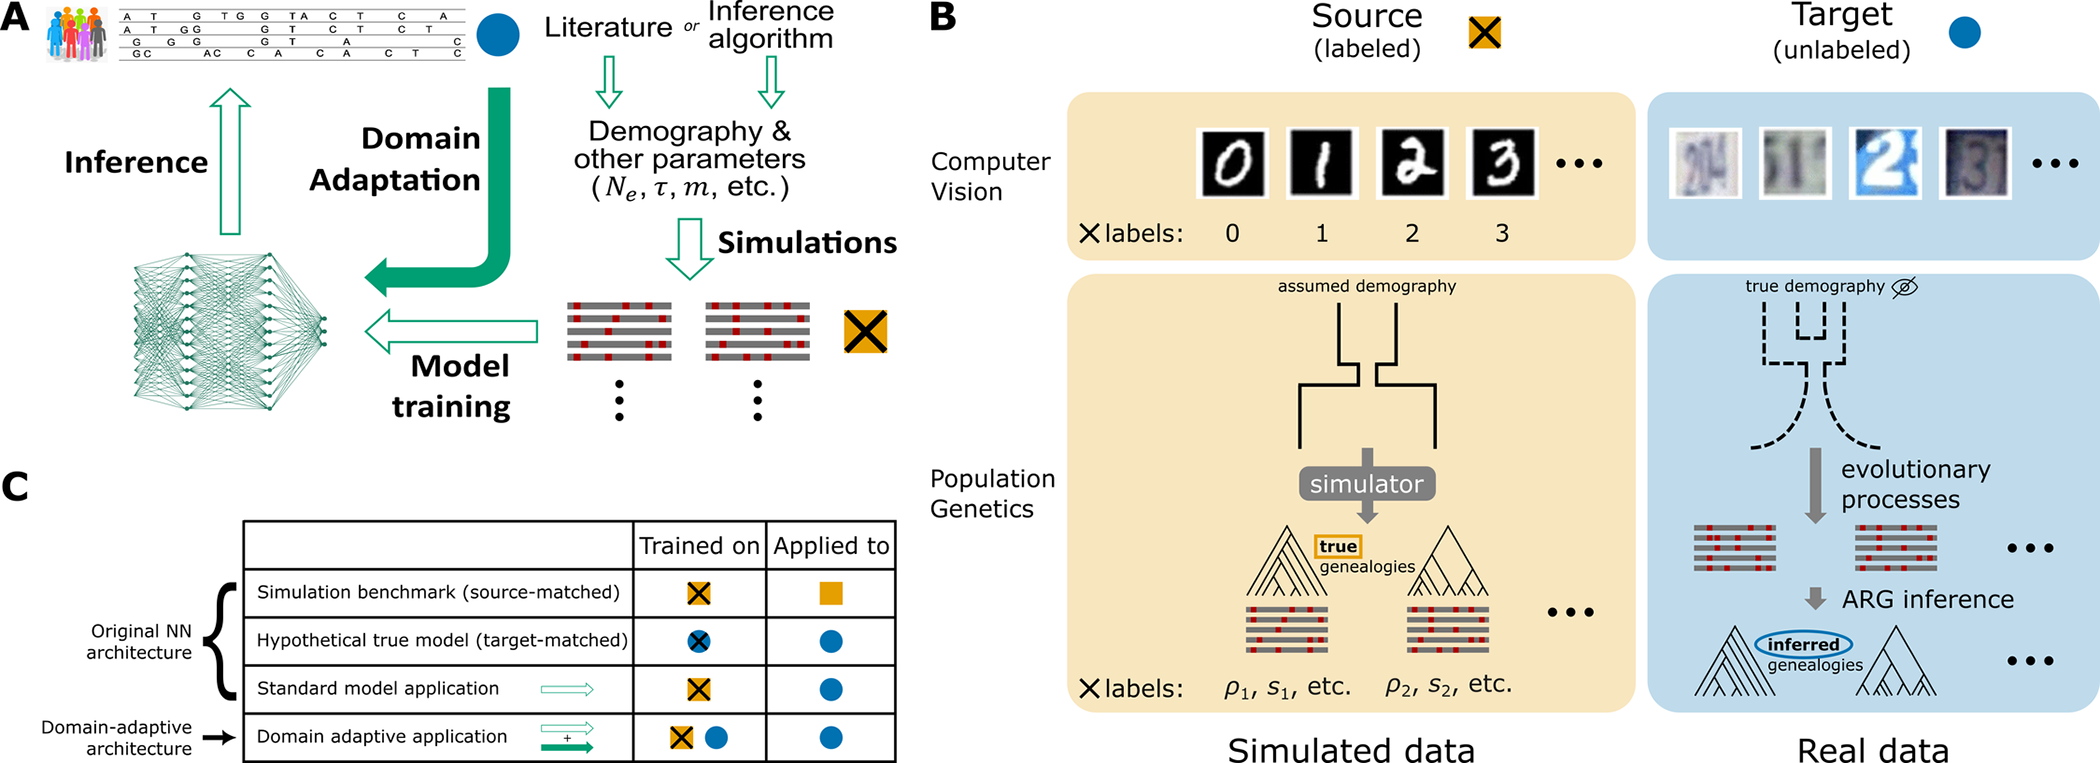
\includegraphics[width=\textwidth]{DA_figs/DA_F1.PNG}
    \caption[Unsupervised domain adaptation in the context of population genetic inference.]{\textbf{Unsupervised domain adaptation in the context of population genetic inference.} \textbf{A)} A high-level overview of the supervised machine-learning approach for population genetic inference and how domain adaptation fits into the paradigm. \textbf{B)} Example formulations of the unsupervised domain adaptation problem with application to computer vision and population genetics. Note that in the specific case of \ac{SIA}, which uses features of the \ac{ARG}, the source domain data always consist of true genealogies generated in simulations, whereas the target domain data always consist of inferred genealogies reconstructed from observed sequence data. \textbf{C)} Four benchmarking scenarios considered in this study. The original model was both trained and tested on source domain data (simulation benchmark), both trained and tested on target domain data (hypothetical true model), or trained on source domain data but applied to target domain data (standard model application). These three cases contextualize the performance of the domain-adaptive model (see \nameref{DA-methods} for details). Gold squares represent source domain data, blue circles represent target domain data and crosses ($\mathbf{\times}$) represent labels.}
    \label{fig:DA-F1}
\end{figure}

At the same time, this paradigm is highly dependent on well-specified models for simulation (\cite{korfmann_deep_2023}). If the simulation assumptions do not match the underlying generative process of the real data -- that is, in the presence of \textit{simulation mis-specification} -- the trained deep-learning model may reflect the biases in the simulated data and perform poorly on real data. Indeed, previous studies have shown that, despite being robust to mild to moderate levels of mis-specification, performance inevitably degrades when the mismatch becomes severe (\cite{adrion_predicting_2020,hejase_deep-learning_2022}).

In a typical workflow, key simulation parameters such as the mutation rate, recombination rate, and parameters of the demographic model are either estimated from the data or obtained from the literature (Fig. \ref{fig:DA-F1}A; \cite{adrion_community-maintained_2020,lauterbur_expanding_2022}). Sometimes these parameters are allowed to vary during simulation, and sometimes investigators evaluate the sensitivity of predictions to departures from the assumed range, but there is typically no way to ensure that the ranges considered are adequately large. Moreover, these benchmarks do not usually account for under-parameterization of the demographic model. Particularly in the case of non-model organisms, the quality of the estimates can be further limited by the availability of data. Overall, some degree of mis-specification in the simulated training data is impossible to avoid.

One way to mitigate the effects of simulation mis-specification would be to engineer a simulator to force the simulated data to be compatible with real data. For example, one could simulate from an overdispersed distribution of parameters followed by a rejection sampling step (based on summary statistics) as in \acf{ABC} methods, or one could use a \ac{GAN} (\cite{wang_automatic_2021}) to mimic the real data. These methods tend to be costly, however. For example, \ac{ABC} methods scale poorly with the dimensionality of the parameter space, and \acp{GAN} are notoriously hard to train.

Here we consider the alternative approach of adopting a deep-learning model that is explicitly designed to account for and mitigate the mismatch between simulated and real data (Fig. \ref{fig:DA-F1}A). A standard machine learning model aims to make accurate predictions on data following the same probability distribution as the training instances. In contrast, the task of building well-performing models for a target dataset that has a \textit{different} distribution from the training dataset is termed “domain adaptation” in the machine-learning literature (\cite{csurka_comprehensive_2017,wilson_survey_2020}). A typical setting of interest for domain adaptation is image classification (Fig. \ref{fig:DA-F1}B). For example, suppose a digit-recognition model is needed for the Street View House Numbers (SVHN) dataset (the “target domain”), but abundant labeled training data is only available from the MNIST dataset of handwritten digits (the “source domain”). In this case, a method needs to train on one dataset and perform well on another, despite systematic differences between the two data distributions.

Various strategies for domain adaptation have been introduced. Prior to the advent of deep learning, early methods focused on reweighting training instances according to their likelihoods of being a source or target example (\cite{shimodaira_improving_2000,dai_boosting_2007}) or explicitly manipulating a feature space through augmentation (\cite{daume_iii_frustratingly_2009}), alignment (\cite{fernando_unsupervised_2013,sun_return_2016}) or transformation (\cite{pan_domain_2011}). Recently, specialized neural network architectures have been developed for deep domain adaptation. Most model architectures of this kind share the common goal of learning a “domain-invariant” representation of the data through a feature extractor neural network, for example, by minimizing domain divergence (\cite{rozantsev_beyond_2019}), by adversarial training (\cite{ganin_unsupervised_2014,liu_coupled_2016}) or through an auxiliary reconstruction task (\cite{ghifary_deep_2016}). Domain adaptation so far has been most widely applied in the fields of computer vision (e.g., using stock photos for semantic segmentation of real photos) and natural language processing (e.g., using Amazon product reviews for sentiment analysis of movies and TV shows) where large, heterogeneous datasets are common but producing labeled training examples can be labor intensive (\cite{wilson_survey_2020}). More recently, deep domain adaptation has been used in regulatory genomics to enable cross-species transcription-factor-binding-site prediction (\cite{cochran_domain-adaptive_2022}).

In this work, we reframe the simulation mis-specification problem in population genetics as an unsupervised domain adaptation problem -- unsupervised in the sense that data from the target domain is not labeled (Fig. \ref{fig:DA-F1}B). In particular, we use population-genetic simulations to obtain large amounts of perfectly labeled training data in the source domain. We then seek to apply the trained model to unlabeled real data in the target domain. We use domain adaptation techniques to explicitly account for the mismatch between these two domains when training the model.

To demonstrate the feasibility of this approach, we incorporated a domain-adaptive neural network architecture into two published deep learning models for population genetic inference: 1) SIA (\cite{hejase_deep-learning_2022}), which identifies selective sweeps based on the \acf{ARG}, and 2) ReLERNN (\cite{adrion_predicting_2020}), which infers recombination rates from raw genotypic data. Through extensive simulation studies, we demonstrated that the domain adaptive versions of the models significantly outperformed the standard versions under realistic scenarios of simulation mis-specification. Our domain-adaptive framework for utilizing mis-specified synthetic data for supervised learning opens the door to many more applications in population genetics.

\section{Results}

\subsection{Experimental design}
We created domain-adaptive versions of the \ac{SIA} and ReLERNN models, each of which employed a \acf{GRL} (\cite{ganin_unsupervised_2014}) (Fig. \ref{fig:DA-F2}A\&B). As noted, the goal of domain adaptation is to establish a “domain-invariant” representation of the data (Fig. \ref{fig:DA-F1}A). Our neural networks consist of two major components: the original networks (“feature extractor” in green and “label predictor” in blue in Fig. \ref{fig:DA-F2}A\&B), which are applied only to labeled examples from the “source” (simulated) domain; and alternative branches (“domain classifier” in yellow in Fig. \ref{fig:DA-F2}A\&B), which use the same feature-extraction portions of the first networks but have the distinct goal of distinguishing data from the “source” (simulated) and “target” (real) domains (they are applied to both). When the neural network is trained by back-propagation, the \ac{GRL} reverses the sign of the gradient for the feature extractor with respect to the domain-classifier loss. By doing so, the \ac{GRL} systematically undermines this secondary goal of distinguishing the two domains (Fig. \ref{fig:DA-F2}, see \nameref{DA-methods} for details), and therefore promotes domain invariance in feature extraction.

\begin{figure}
    \centering
    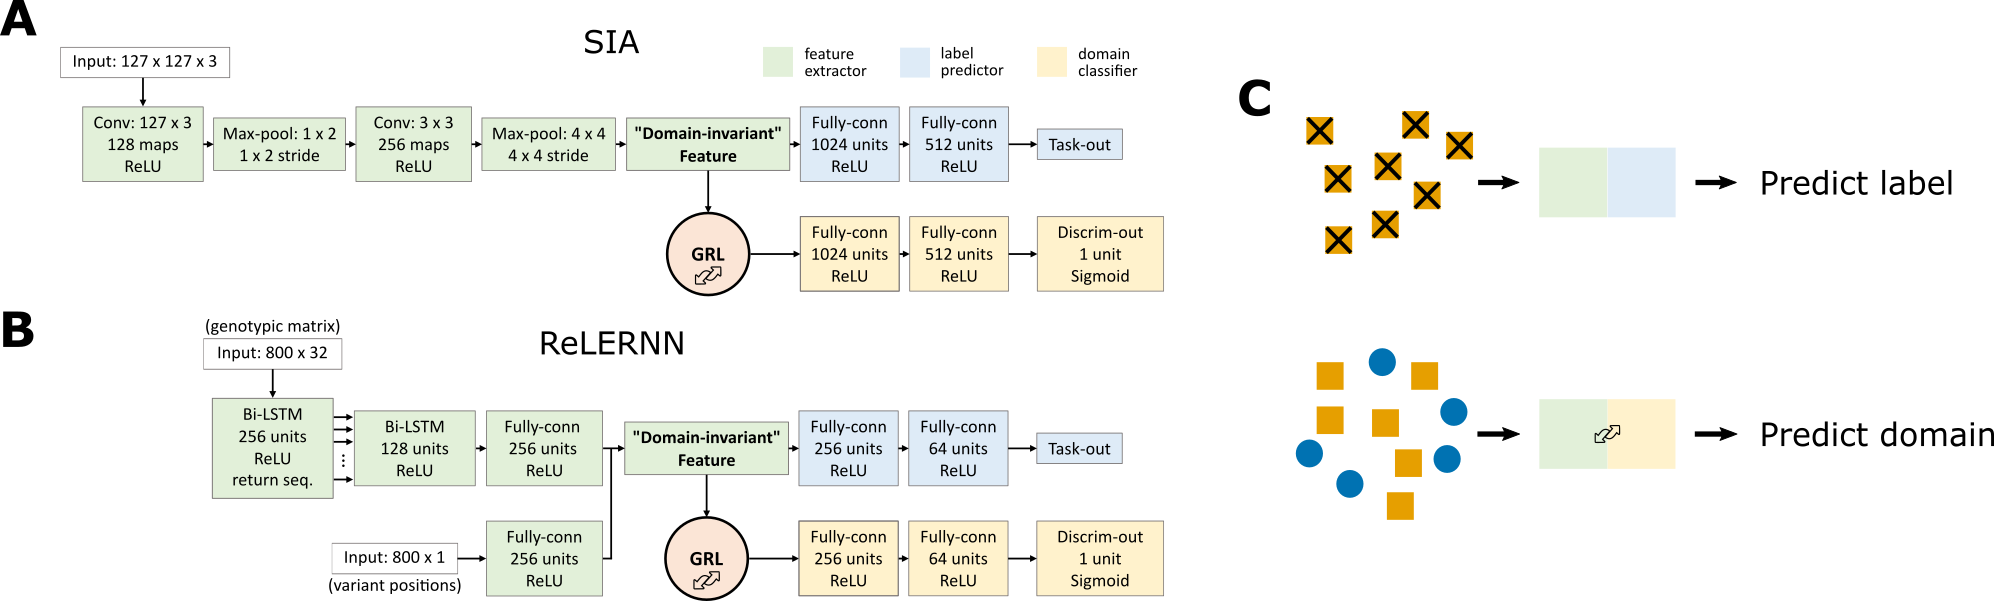
\includegraphics[width=\textwidth]{DA_figs/DA_F2.PNG}
    \caption[Neural network architecture for domain adaptation.]{\textbf{Neural network architecture for domain adaptation.} The model architectures incorporating \acfp{GRL} for \textbf{A)} \ac{SIA} and \textbf{B)} ReLERNN. The feature extractor of \ac{SIA} contains $1.49 \times 10^5$ trainable parameters, whereas the label predictor and domain classifier contains $1.22 \times 10^8$ each. The feature extractor of ReLERNN contains $1.52 \times 10^6$ trainable parameters, whereas the label predictor and domain classifier contains $1.49 \times 10^5$ each. Note that the total number of trainable parameters includes those in batch normalization layers. \textbf{C)} When training the networks, each minibatch of training data consists of two components: (1) labeled data from the source domain fed through the feature extractor and the label predictor; and (2) a mixture of unlabeled data from both the source and target domains fed through the feature extractor and the domain classifier. The first component trains the model to perform its designated task. However, the \ac{GRL} inverts the loss function for the second component, discouraging the model from differentiating the two domains and leading to the extraction of “domain-invariant” features.}
    \label{fig:DA-F2}
\end{figure}

We designed two sets of benchmark experiments to assess the performance of the domain-adaptive models relative to the standard models. In both cases, we tested the methods using “real” data in the target domain that was actually generated by simulation, but included features not considered by the simpler simulator used for the source domain. In the first set of experiments, background selection was present in the target domain but not the source domain. In the second set of experiments, the demographic model used for the source-domain simulations was estimated from “real” data generated under a more complex demographic model and was therefore somewhat mis-specified (as detailed below). Below we refer to these as the “background selection” and “demography mis-specification” experiments.

\subsection{Performance of domain-adaptive \ac{SIA} model}
We compared the performance of the \acf{dadaSIA} model to that of the standard \ac{SIA} model on held-out “real” data, considering both a classification (distinguishing selective sweeps from neutrality) and a regression (inferring selection coefficients) task. In all cases, we focused on a comparison of the domain-adaptive model to the standard case where a model is simply trained on data from the source domain and then applied to the target domain (“standard model”; Fig. \ref{fig:DA-F1}C). Note that the version of \ac{SIA} used by both the domain-adaptive and standard models includes a variety of minor improvements that led to modest gains in performance over the previously published version (see \textit{Updates to genealogical features and deep learning architecture for the \ac{SIA} model} in \nameref{DA-methods} and Fig. \href{https://journals.plos.org/plosgenetics/article?id=10.1371/journal.pgen.1011032#sec018}{S1B\&C online}). The codebase of the original \ac{SIA} model has been updated accordingly.

For additional context, we also considered the two cases where the training and testing domains matched (“source-matched” or “target-matched”; Fig. \ref{fig:DA-F1}C)—although we note that these cases are not achievable with real data and provide only hypothetical upper bounds on performance. Notably, in the source-matched (or “simulation benchmark”) case, the standard model is both trained and tested with true genealogies from source-domain simulations. By contrast, in the target-matched (or “hypothetical true model”) case, the standard model is trained as if target-domain data with ground-truth selection coefficient labels were available. Since genealogies need to be inferred in the target domain (Fig. \ref{fig:DA-F1}B), the hypothetical true model is both trained and tested with inferred genealogies (see \textit{Setup of benchmarking experiments} in \nameref{DA-methods} for details).

As noted, we considered two types of mis-specification, background selection and demographic mis-specification. In the background selection experiments, the target domain experienced selection in a central “genic” region (following a \acsu{DFE} from \cite{boyko_assessing_2008}), leading to background selection in flanking regions. This genic region was omitted in the source domain. In the demographic mis-specification experiments, the demographic model for source-domain simulations was inferred from “real” data using G-PhoCS (\cite{gronau_bayesian_2011}). Both the real (target domain) and inferred (source domain) models assumed three populations with migration, but the inferred model was under-parameterized and its parameters differed substantially from the real model (Fig. \href{https://journals.plos.org/plosgenetics/article?id=10.1371/journal.pgen.1011032#sec018}{S1A online}) (see \nameref{DA-methods} for details).

In both the background selection and demography mis-specification experiments, and in both the classification and regression tasks, the domain-adaptive \ac{SIA} model substantially improved on the standard model (Fig. \ref{fig:DA-F3}). Indeed, in all cases, the domain-adaptive model (turquoise lines in Fig. \ref{fig:DA-F3}A\&C) nearly achieved the upper bound of the hypothetical true model (dashed gray lines) and clearly outperformed the standard model (gold lines), suggesting that domain adaptation had largely “rescued” \ac{SIA} from the effects of simulation mis-specification (see also Fig. \href{https://journals.plos.org/plosgenetics/article?id=10.1371/journal.pgen.1011032#sec018}{S2C\&D online}). The standard model performed particularly poorly on the regression task (Fig. \ref{fig:DA-F3}B\&D), but the domain-adaptive model achieved substantial improvements, reducing both the absolute error as well as the upward bias of the estimation (Fig. \href{https://journals.plos.org/plosgenetics/article?id=10.1371/journal.pgen.1011032#sec018}{S2C\&D online}).

\begin{figure}
    \centering
    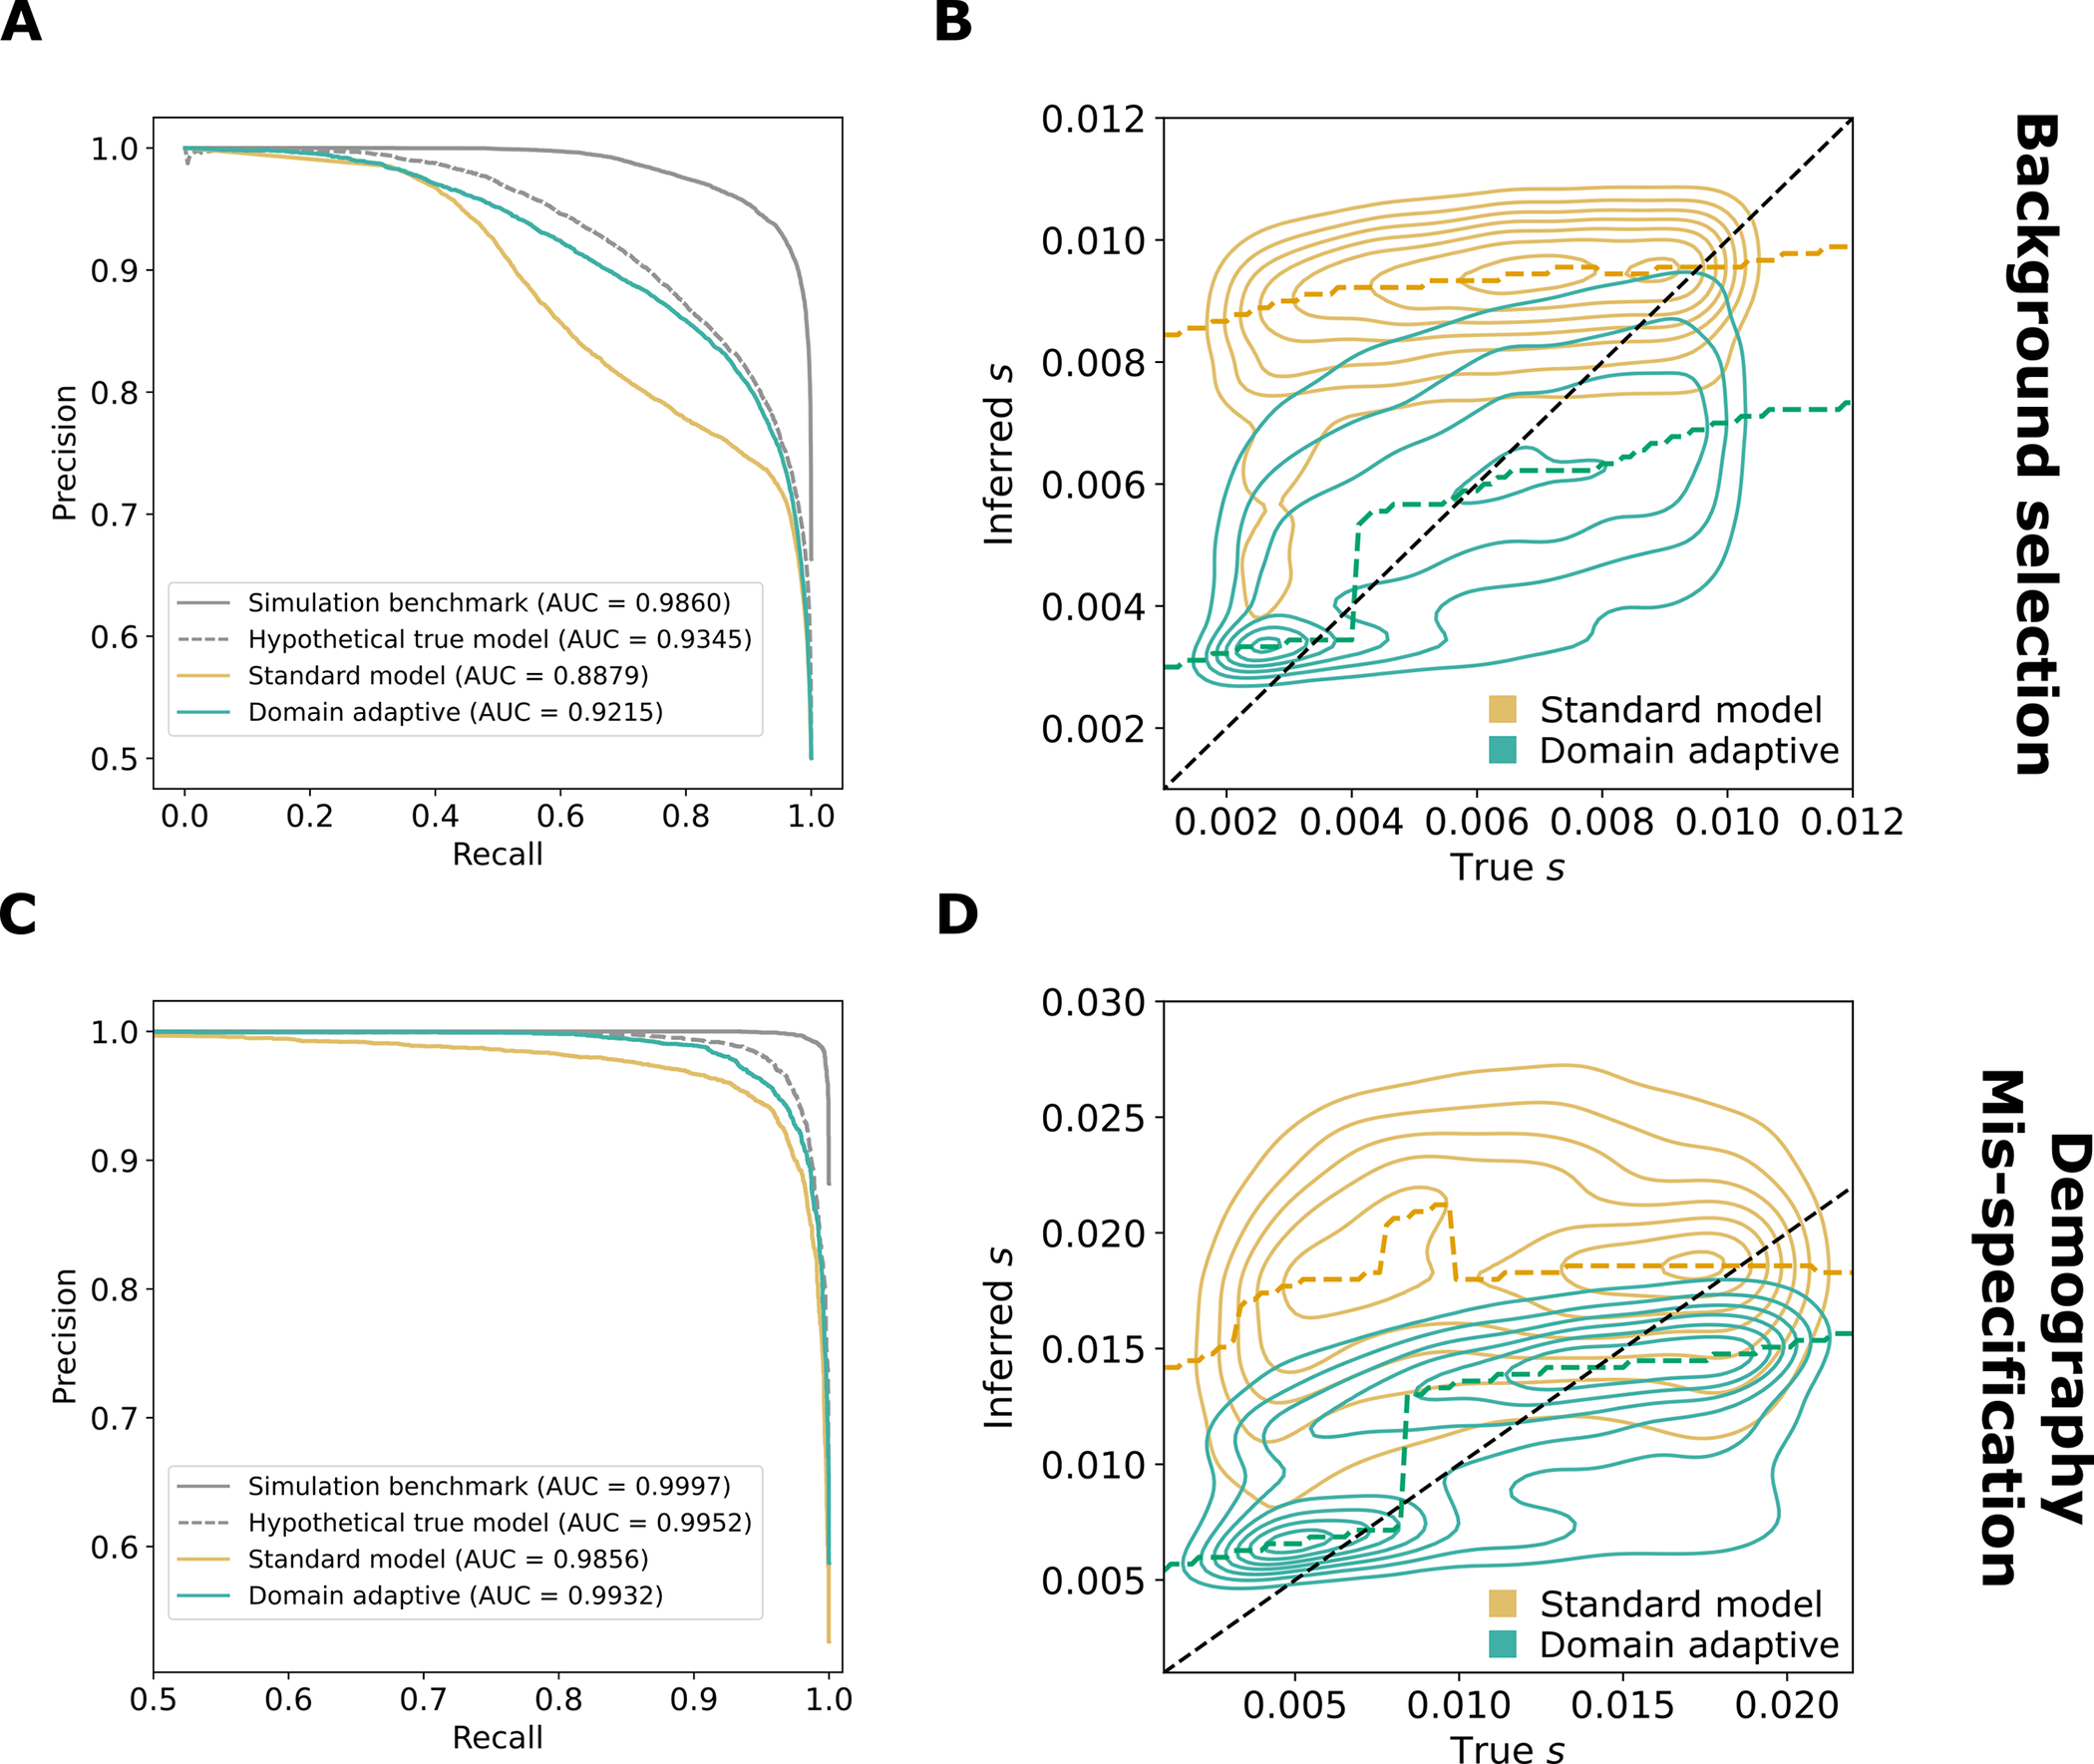
\includegraphics[width=\textwidth]{DA_figs/DA_F3.PNG}
    \caption[Performance of domain-adaptive \ac{SIA} models.]{\textbf{Performance of domain-adaptive \ac{SIA} models.} Results are shown from (\textbf{A}, \textbf{B}) the background-selection and (\textbf{C}, \textbf{D}) the demography-mis-specification experiments. (\textbf{A}, \textbf{C}) Precision-recall curves for sweep classification. (\textbf{B}, \textbf{D}) Contour plots summarizing true (horizontal axis) vs. inferred (vertical axis) selection coefficients ($s$) for the standard (gold) and domain adaptive (turquoise) models as evaluated on the held-out test dataset. The ridge along the horizontal axis of each contour is traced by a dashed line, representing the mode of the inferred value for each true value of $s$. Raw data underlying the contour plots are presented in Fig. \href{https://journals.plos.org/plosgenetics/article?id=10.1371/journal.pgen.1011032\#sec018}{S2 online}. See Fig. \ref{fig:DA-F1}C for definition of the model labels.}
    % https://tex.stackexchange.com/questions/366909/and-other-characters-in-a-url
    \label{fig:DA-F3}
\end{figure}

The comparisons with the simulation benchmark and hypothetical true model were also informative in other ways. Notice that performance in the simulation benchmark case was considerably better than that in all other cases, including the hypothetical true model. For \ac{SIA} in particular, the \ac{ARG} is “known” (fixed in simulation) in the source domain, whereas in the target domain it must be inferred (Fig. \ref{fig:DA-F1}B). Thus, the difference between the simulation benchmark (source-matched) and hypothetical true model (target-matched) cases represents a rough measure of the importance of \ac{ARG} inference error (see \nameref{DA-discussion}). In addition, note that in many studies, benchmarking of population-genetic models is performed using the same, or similar, simulations as those used for training, as with our hypothetical true model. Thus, the difference between the hypothetical true model and the standard model is representative of the degree to which benchmarks of this kind may be overly optimistic about performance, depending on the degree to which the simulations are mis-specified.

We further investigated the effect of imbalanced training data from the target domain on the performance of the domain-adaptive model in the context of sweep classification. Despite the ability to simulate perfectly class-balanced labeled data in the source domain, in practice we have no control over whether real data are balanced. Using simulations for the background selection mis-specification experiments, we tested the performance of the domain-adaptive \ac{SIA} model classifying sweeps when trained with unlabeled “real” data under different proportions of sweep vs. neutral examples. While a balanced dataset yielded the best performance, significantly skewed datasets (20\% or 80\% sweep examples) still provided the domain-adaptive model with reasonable improvement upon the standard model (Fig. \href{https://journals.plos.org/plosgenetics/article?id=10.1371/journal.pgen.1011032\#sec018}{S3A\&B online}). The exception appeared to be when the target domain data consisted entirely of sweep examples (100\% sweep). Although highly unrealistic, this scenario demonstrates that the domain-adaptive model can underperform the standard model when the target domain data follow a radically different distribution.

Another type of imbalance arises if only a limited amount of target domain data is available to train the domain-adaptive model. Using the same set of simulations for the background selection mis-specification experiments, we tested the performance of the domain-adaptive \ac{SIA} model when trained with less target domain data. With the target domain data at only 10\% of the source domain data (source:target ratio = 10:1), the model suffered a noticeable drop in performance yet still maintained a clear advantage over the standard model (Fig. \href{https://journals.plos.org/plosgenetics/article?id=10.1371/journal.pgen.1011032\#sec018}{S3C-E online}). We did not examine the case where there is more target domain than source domain data, since one could always simulate additional source domain data to match the size of the target domain. In summary, our experiments suggest that domain adaptation can accommodate reduced or imbalanced data for the target domain but there is a cost in performance if the reduction or imbalance is extreme.

\subsection{Performance of domain-adaptive ReLERNN model}
We performed a parallel set of experiments with a domain-adaptive version of ReLERNN. In this case, the background selection experiment was essentially the same as for \ac{SIA}, but we used a simpler design for the demography mis-specification experiment, following \cite{adrion_predicting_2020}. Briefly, the “real” (target domain) data was generated according to the out-of-Africa European demographic model estimated by \cite{tennessen_evolution_2012}. By contrast, the simulated data for the source domain simply assumed a constant-sized panmictic population at equilibrium with $N_e=\frac{\hat{\theta}_W}{4\mu}$, where  $\hat{\theta}_W$ is the Watterson estimator obtained from the “real” data (see \nameref{DA-methods} for details).

Similar to our results for \ac{SIA}, the domain-adaptive ReLERNN model both reduced the \ac{MAE} and corrected for the downward bias in recombination-rate estimates compared to the standard model (Figs. \ref{fig:DA-F4} and \href{https://journals.plos.org/plosgenetics/article?id=10.1371/journal.pgen.1011032#sec018}{S6 online}). In the background-selection experiment, the standard ReLERNN model performed quite well (Figs. \ref{fig:DA-F4}A and \href{https://journals.plos.org/plosgenetics/article?id=10.1371/journal.pgen.1011032#sec018}{S6A online}, $\mathrm{MAE} = 5.60\times 10^{-9}$), but the domain-adaptive ReLERNN model nonetheless further reduced the MAE to $4.41\times 10^{-9}$ (Fig. \href{https://journals.plos.org/plosgenetics/article?id=10.1371/journal.pgen.1011032#sec018}{S6C online}, Welch’s $t$-test: $n = 25,000$, $t =31.0$, $p<10^{-208}$). The advantage of the domain-adaptive model was more apparent in the demography-mis-specification experiment (Figs. \ref{fig:DA-F4}B and \href{https://journals.plos.org/plosgenetics/article?id=10.1371/journal.pgen.1011032#sec018}{S6B online}), where it reduced the MAE from $8.06\times 10^{-9}$ to $5.45\times 10^{-9}$ (Fig. \href{https://journals.plos.org/plosgenetics/article?id=10.1371/journal.pgen.1011032#sec018}{S6D online}, Welch’s $t$-test, $n = 25,000$, $t = 72.4$, $p<10^{-323}$). Notably, our results for the standard model in the demography-mis-specification experiment were highly similar to those reported by \cite{adrion_predicting_2020}, including the approximate mean and range of the raw error (compare \href{https://academic.oup.com/view-large/figure/204168641/msaa038f4.tif}{Fig. 4A} from \cite{adrion_predicting_2020} and Fig. \href{https://journals.plos.org/plosgenetics/article?id=10.1371/journal.pgen.1011032#sec018}{S6D online}), as well as the downward bias.

\begin{figure}[h]
    \centering
    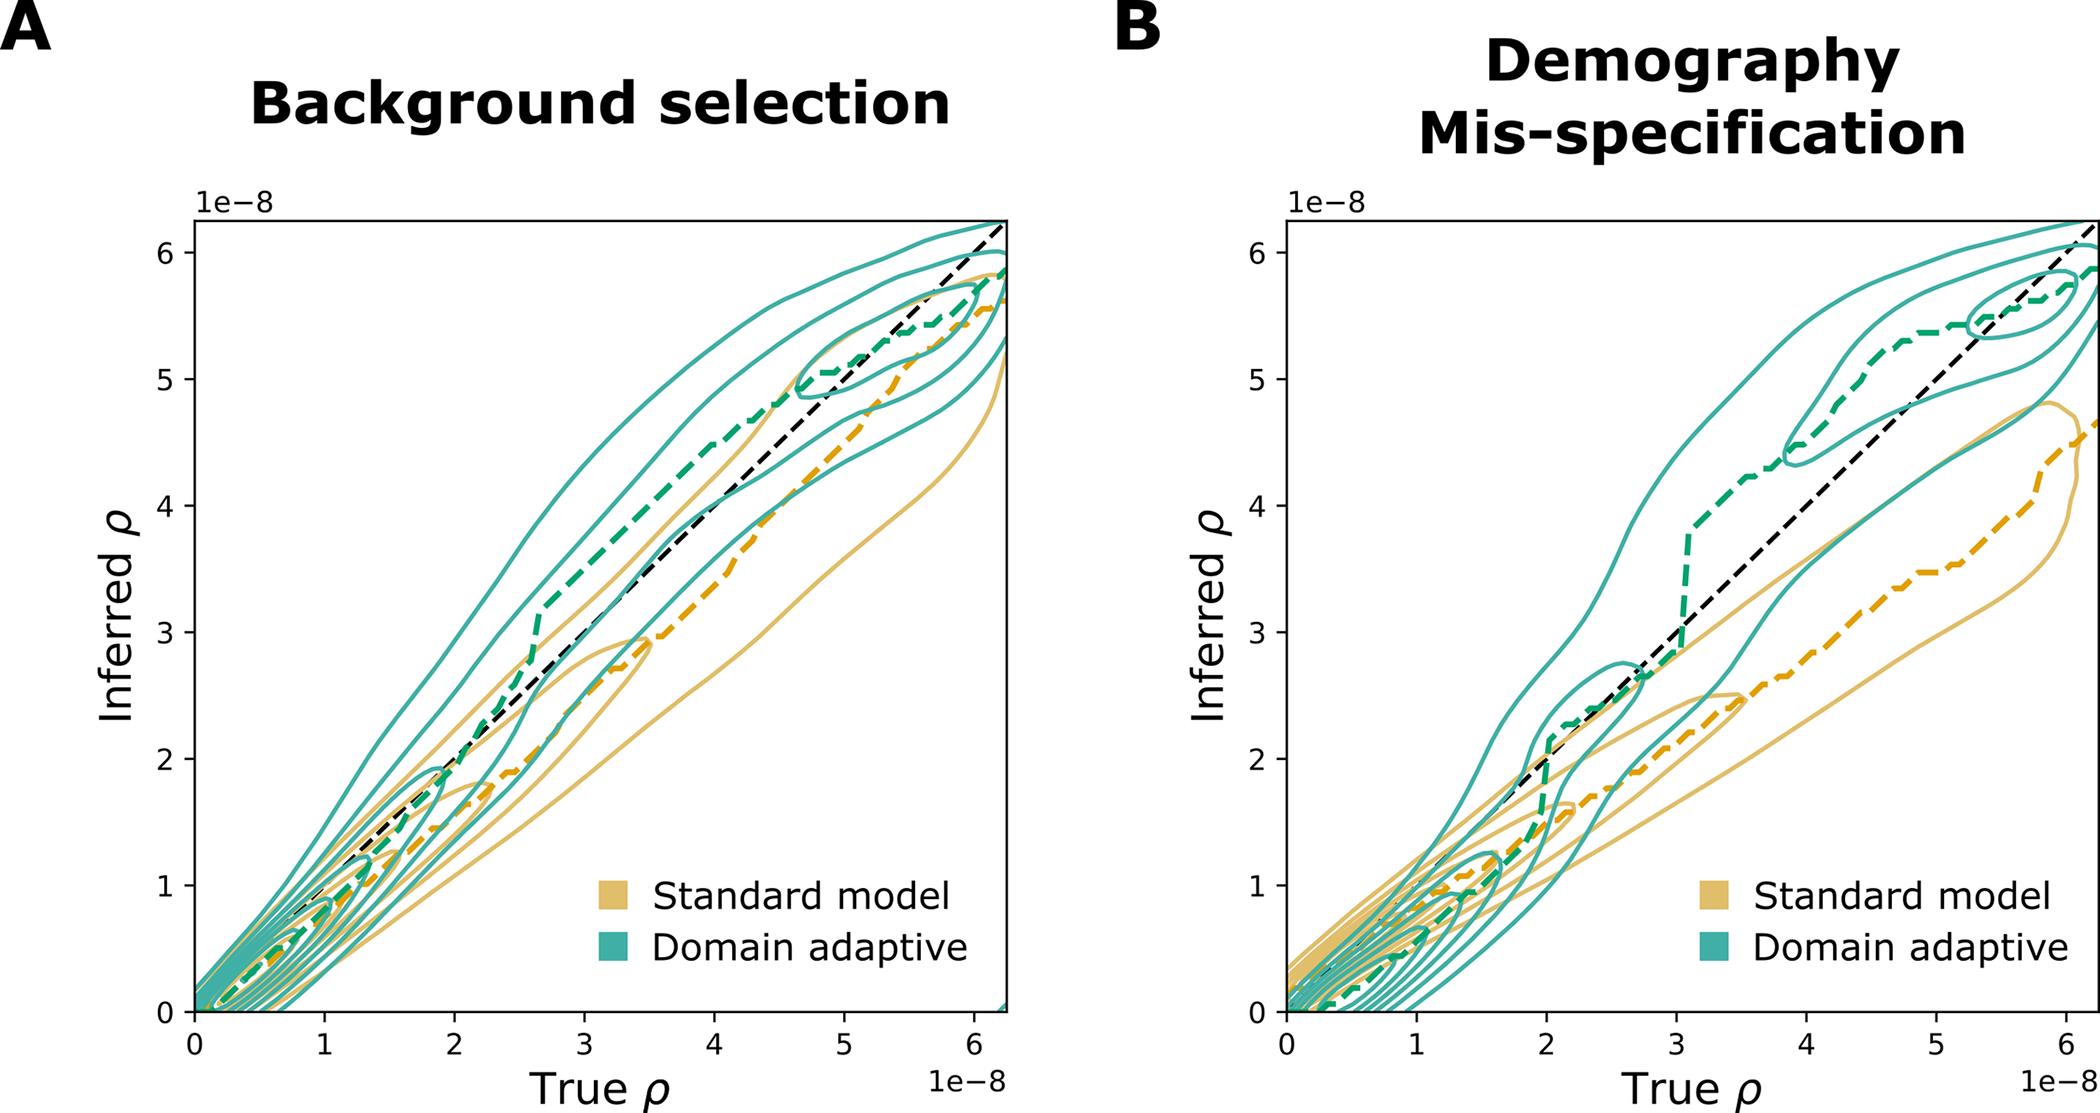
\includegraphics[width=\textwidth]{DA_figs/DA_F4.PNG}
    \caption[Performance of domain-adaptive ReLERNN models.]{\textbf{Performance of domain-adaptive ReLERNN models.} Results are shown from (\textbf{A}) the background-selection and (\textbf{B}) the demography-mis-specification experiments. Each contour plot summarizes true (horizontal axis) vs. inferred (vertical axis) recombination rates ($\rho$) for the standard (gold) and domain adaptive (turquoise) models as evaluated on the held-out test dataset. The ridge along the horizontal axis of each contour is traced by a dashed line, representing the mode of the inferred value for each true value of $\rho$. Raw data underlying the contour plots are presented in Fig. \href{https://journals.plos.org/plosgenetics/article?id=10.1371/journal.pgen.1011032\#sec018}{S6 online}.}
    \label{fig:DA-F4}
\end{figure}

Interestingly, \cite{adrion_predicting_2020} observed that ReLERNN was sometimes more strongly influenced by demographic mis-specification than unsupervised methods such as LDhelmet, even though it still performed better in terms of absolute error. The addition of domain adaptation appears to considerably mitigate this susceptibility to demographic mis-specification, making an excellent method even stronger.

\subsection{Efficacy of domain adaptation under various degrees of simulation mis-specification}
So far, we have examined scenarios of relatively modest simulation mis-specifica\\-tion, likely to be encountered in real applications. While domain adaptation appeared to be effective in these cases, we expect a limit to its capability when mis-specification is extreme. We therefore carried out a series of experiments to probe the performance of the \ac{dadaSIA} model under increasingly severe simulation mis-specification (Fig. \href{https://journals.plos.org/plosgenetics/article?id=10.1371/journal.pgen.1011032#sec018}{S4 online}, also see \nameref{DA-methods}).

We found that \ac{dadaSIA} exhibited good performance when mis-specification was caused by genealogy inference alone or by light to moderate bottlenecks. As the bottleneck became more severe, its performance deteriorated, but even with a 5\% bottleneck, \ac{dadaSIA} still outperformed the standard model (Fig. \ref{fig:DA-F5}). To examine the limits of the method, we tested an extreme scenario with the 5\% bottleneck, background selection and an 8-fold mis-specification of recombination rate. In this case, the model performed poorly, having virtually no power to classify sweeps and large errors in its selection coefficient estimates (Fig. \ref{fig:DA-F5}). This example demonstrates that, while domain adaptation is useful over a broad range of mis-specification levels, it eventually does fail when mis-specification becomes extreme.

\begin{figure}
    \centering
    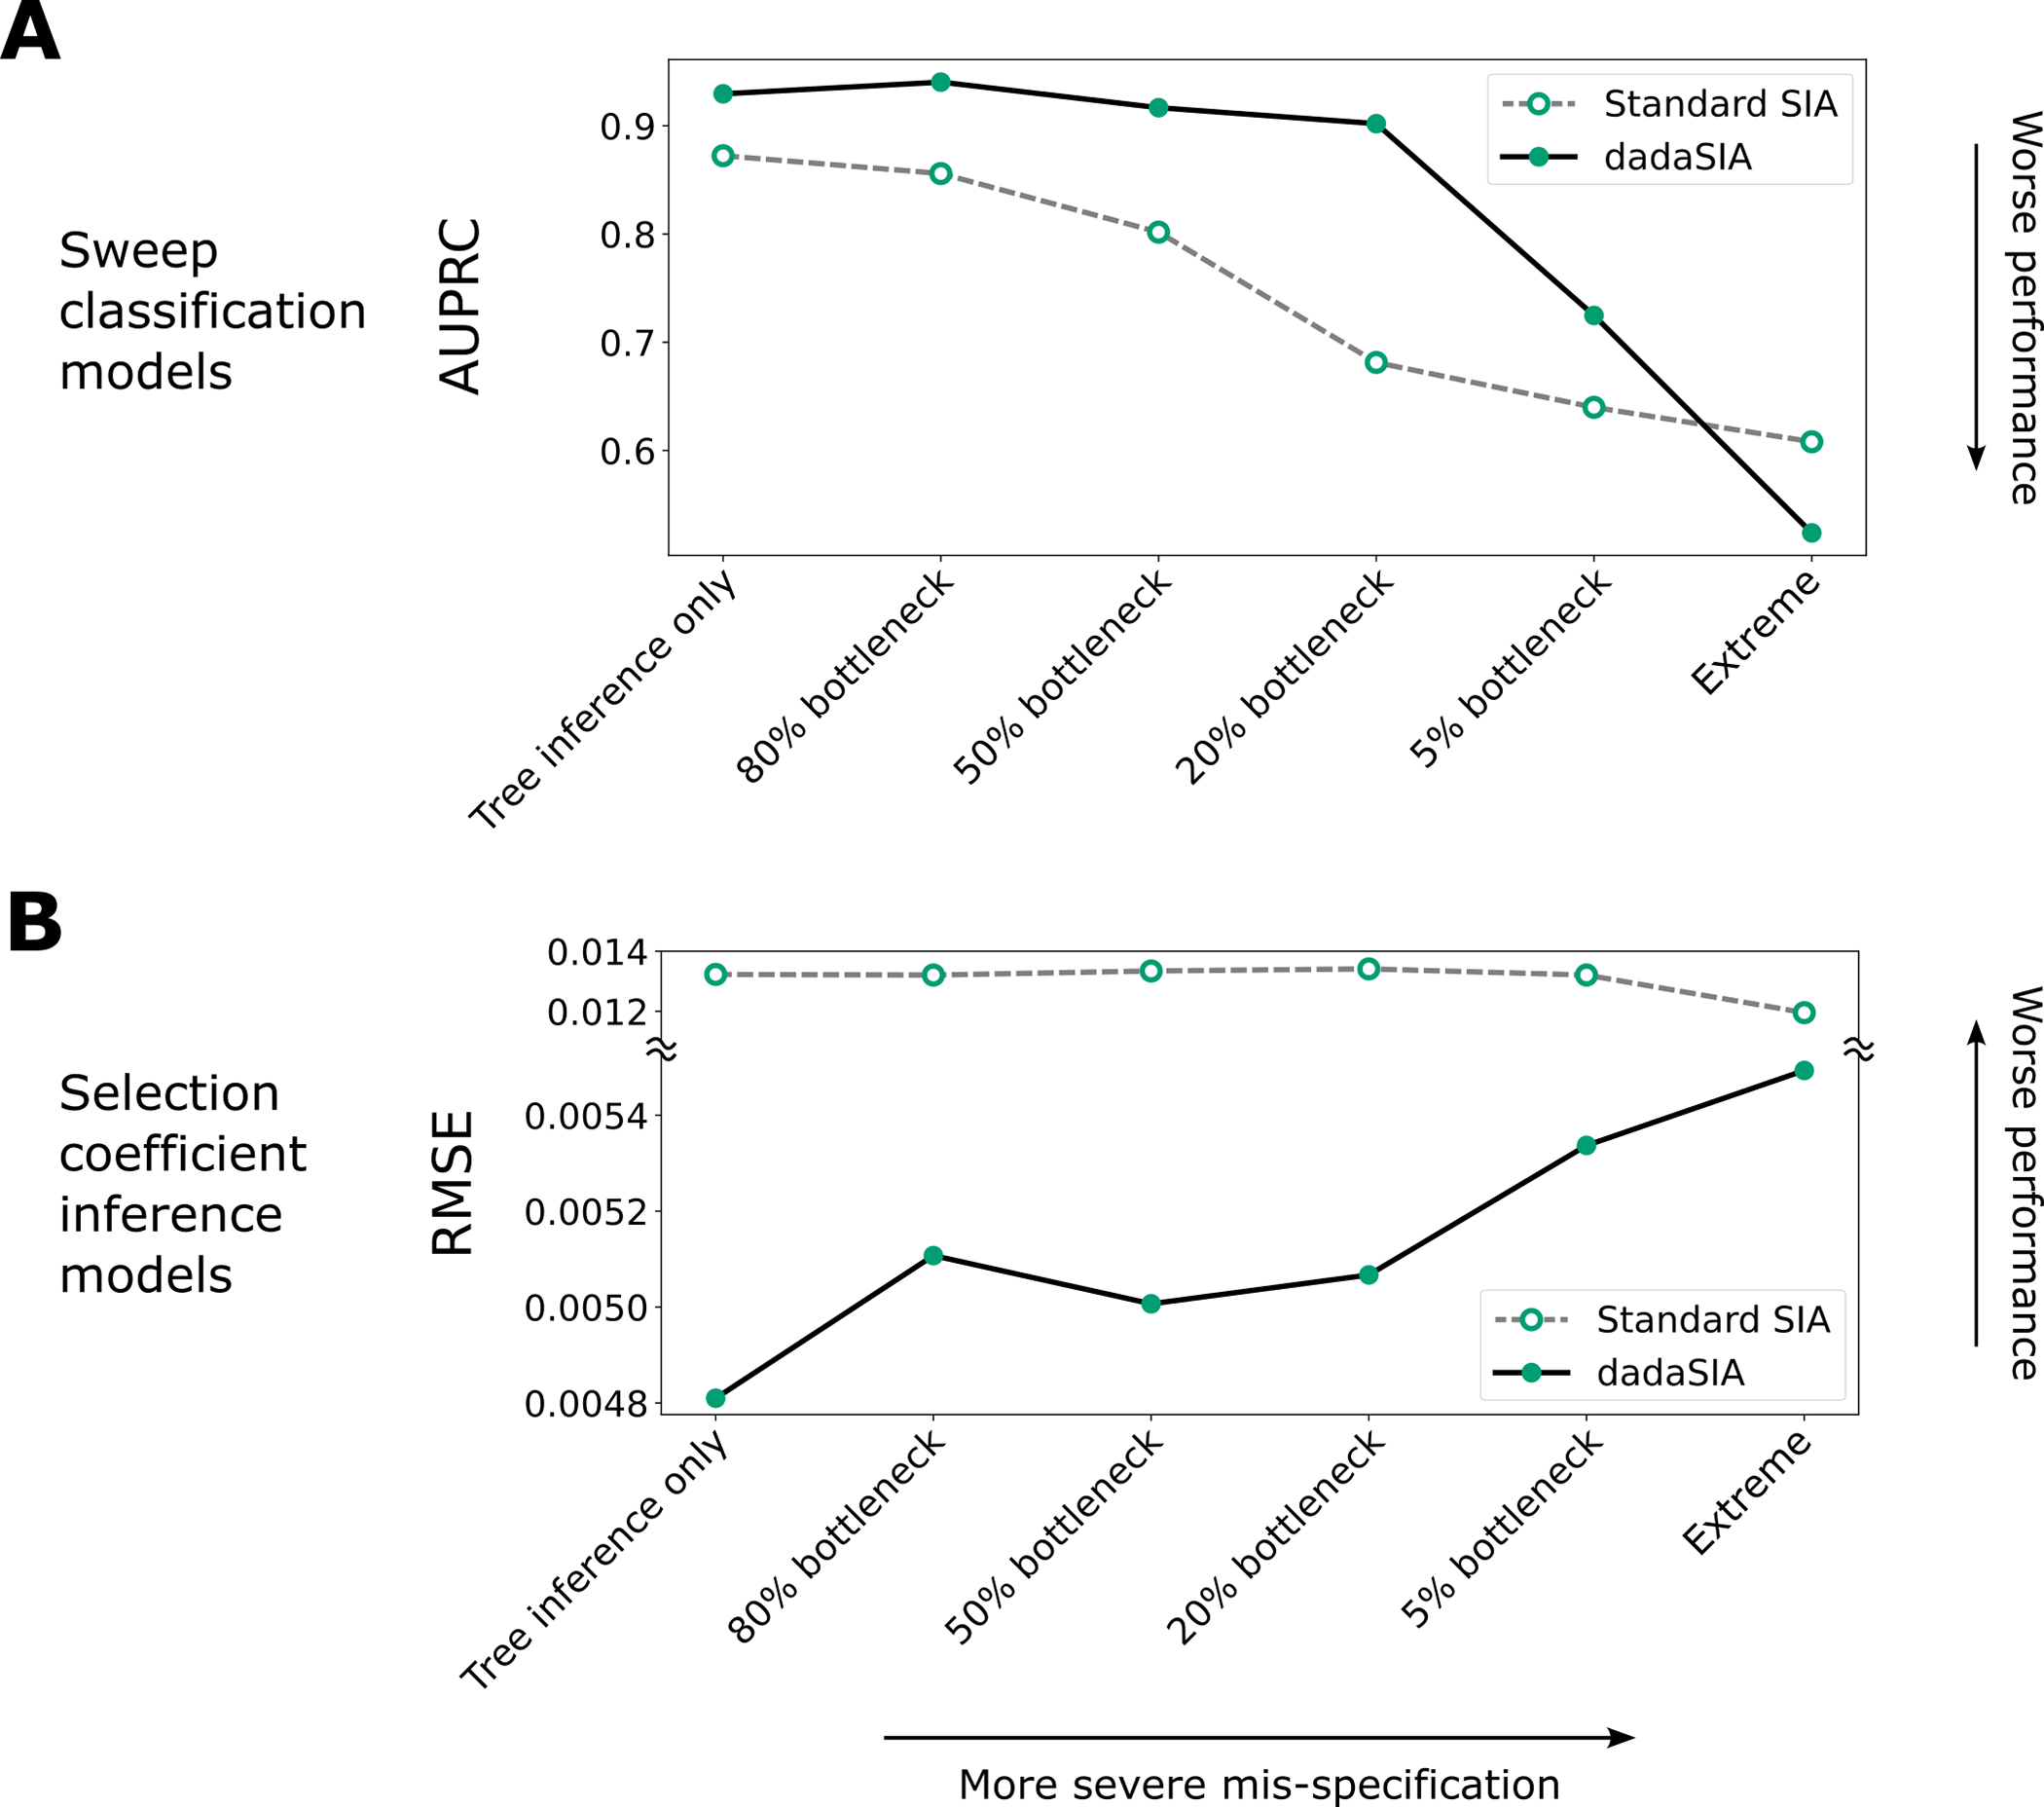
\includegraphics[width=\textwidth]{DA_figs/DA_F5.PNG}
    \caption[Performance of \acf{dadaSIA} model with different degrees of mis-specification.]{\textbf{Performance of \acf{dadaSIA} model with different degrees of mis-specification.} The performance of the model on the sweep classification task is quantified by the \ac{AUPRC} (\textbf{A}). Performance on the selection-coefficient inference task is quantified by \ac{RMSE} (\textbf{B}). In the “tree inference only” case, there is no mis-specification other than that caused by error in genealogy inference. In the “extreme” case, mis-specification consists of a 5\% bottleneck, background selection and an 8-fold mis-specification in recombination rate. See Fig. \href{https://journals.plos.org/plosgenetics/article?id=10.1371/journal.pgen.1011032\#sec018}{S4 online} for illustrations of the different bottlenecks and \nameref{DA-methods} for details.}
    \label{fig:DA-F5}
\end{figure}

Does domain adaptation compromise performance at the opposite extreme, where there is little or no simulation mis-specification? To address this question, we tested the standard and domain-adaptive ReLERNN models in a setting without any simulation mis-specification. We focused here on ReLERNN, which directly uses raw genotypic data, as opposed to SIA, which always has some mis-specification due to genealogy inference error. We observed that the standard and domain-adaptive ReLERNN models performed nearly identically when no mis-specification was present, with only minor decreases in performance (Fig. \href{https://journals.plos.org/plosgenetics/article?id=10.1371/journal.pgen.1011032#sec018}{S7 online}). Thus, there is perhaps some cost in using domain adaptation when it is not needed, but, at least in our case, that cost appears to be slight.

\subsection{Application of domain-adaptive \ac{SIA} to real data}
In applications to real data, the true selection coefficient is not known, so it is impossible to perform a definitive comparison of methods. Nevertheless, it can be informative to evaluate the degree to which alternative methods are concordant, especially with consideration of their relative performance in simulation studies.

Toward this end, we re-applied our \acf{dadaSIA} model to several loci in the human genome that we previously analyzed with \ac{SIA} (\cite{hejase_deep-learning_2022}), using whole-genome sequence data from the 1000 Genomes CEU population (\cite{auton_global_2015}). For the target domain, we sampled genealogies from genome-wide \acp{ARG} inferred from the individual sequences (see \nameref{DA-methods}). The putative causal loci analyzed included \acp{SNP} at the \textit{LCT} gene (\cite{bersaglieri_genetic_2004}), one of the best-studied cases of selective sweeps in the human genome; at the disease-associated genes \textit{TCF7L2} (\cite{lyssenko_mechanisms_2007}), \textit{ANKK1} (\cite{spellicy_variant_2014}) and \textit{FTO} (\cite{frayling_common_2007}); at the pigmentation genes \textit{KITLG} (\cite{sulem_genetic_2007}), \textit{ASIP} (\cite{eriksson_web-based_2010}), \textit{TYR} (\cite{sulem_genetic_2007,eriksson_web-based_2010}), \textit{OCA2} (\cite{han_genome-wide_2008,sturm_single_2008}), \textit{TYRP1} (\cite{kenny_melanesian_2012}) and \textit{TTC3} (\cite{liu_digital_2010}), which were also analyzed by \cite{stern_approximate_2019}; and at the genes \textit{MC1R} (\cite{sulem_genetic_2007,han_genome-wide_2008}) and \textit{ABCC11} (\cite{yoshiura_snp_2006}), where \ac{SIA} reported novel signals of selection.

We found that \ac{dadaSIA} generally made similar predictions to \ac{SIA} at these \acp{SNP}, but there were some notable differences. The seven loci predicted by SIA to be sweeps were also predicted by dadaSIA to be sweeps (Table \ref{tab:DA-T1}), although \ac{dadaSIA} always reported higher confidence in these predictions (with probability of neutrality, $P_{\mathrm{neu}}<10^{-2}$ in all cases) than did \ac{SIA} ($P_{\mathrm{neu}}$ up to 0.384 for \textit{TYR}). The five loci predicted by \ac{SIA} not to be sweeps were also predicted by \ac{dadaSIA} not to be sweeps ($P_{\mathrm{neu}}>0.5$). At \textit{LCT}, the strongest sweep considered, the selection coefficient ($s$) estimated by \ac{dadaSIA} remained very close to \ac{SIA}’s previous estimate of $s = 0.01$ and also close to several prior estimates (\cite{bersaglieri_genetic_2004,mathieson_estimating_2020,mathieson_fads1_2018}). In all other cases, the estimate from \ac{SIA} was somewhat revised by \ac{dadaSIA}, generally by factors of about 2-3. Importantly, in all cases, the estimates from \ac{dadaSIA} remained much closer to those from \ac{SIA} than to estimates by other methods (Table \ref{tab:DA-T1}). Together, these observations suggest that the addition of domain adaptation does not radically alter \ac{SIA}’s predictions for real data but may in some cases improve them (see \nameref{DA-discussion}).

\begin{sidewaystable}
    \centering
    \caption{Selection coefficients in the European population estimated by domain-adaptive \ac{SIA} compared to previous estimates.}
    \vspace{5mm}
    \begin{tabular}{l | l | m{5cm} l m{8cm}}
    \hline
    % https://tex.stackexchange.com/questions/269547/rowcolor-for-a-multirow
       & & \multicolumn{3}{c}{\textbf{Estimates of selection coefficient}} \\ \cline{3-5}
      \rowcolor{white} \multirow{-2}{*}{\textbf{Gene}} & \multirow{-2}{*}{\textbf{\ac{SNP}}} & \textbf{Domain-adaptive SIA} & \textbf{SIA}* & \textbf{Previous estimates} \\ \hline
      \textit{KITLG} & rs12821256 & 0.0035 & 0.0019 & 0.0161 (\cite{stern_approximate_2019}) \\
      \textit{ASIP} & rs619865 & 0.0057 & 0.0019 & 0.0974 (\cite{stern_approximate_2019}) \\
      \textit{TYR} & rs1393350 & 0.0028 & 0.0011 & 0.0112 (\cite{stern_approximate_2019}) \\
      \textit{OCA2} & rs12913832 & 0.0093 & 0.0056 & 0.002 (\cite{stern_approximate_2019}); 0.036 (\cite{wilde_direct_2014}) \\
      \textit{MC1R} & rs1805007 & 0.0027 & 0.0037 & No selection (\cite{harding_evidence_2000}) \\
      \textit{ABCC11} & rs17822931 & 0.0020 & 0.00035 & $\approx$ 0.01 in East Asian (\cite{ohashi_impact_2011}) \\
      \textit{LCT} & rs4988235 & 0.0097 & 0.010 & $\approx$ 0.01 (\cite{bersaglieri_genetic_2004,mathieson_fads1_2018,mathieson_estimating_2020}) \\
      \textit{TYRP1} & rs13289810 & $P_{\mathrm{neu}}>0.5$ & $P_{\mathrm{neu}}>0.5$ & No selection (\cite{stern_approximate_2019}) \\
      \textit{TTC3} & rs1003719 & $P_{\mathrm{neu}}>0.5$ & $P_{\mathrm{neu}}>0.5$ & No selection (\cite{stern_approximate_2019}) \\
      \textit{TCF7L2} & rs7903146 & $P_{\mathrm{neu}}>0.5$ & $P_{\mathrm{neu}}>0.5$ & N/A \\
      \textit{ANKK1} & rs1800497 & $P_{\mathrm{neu}}>0.5$ & $P_{\mathrm{neu}}>0.5$ & N/A \\
      \textit{FTO} & rs9939609 & $P_{\mathrm{neu}}>0.5$ & $P_{\mathrm{neu}}>0.5$ & N/A \\
      \hline
      \rowcolor{white} \multicolumn{5}{p{20cm}}{*The original \ac{SIA} model in \cite{hejase_deep-learning_2022} uses genealogies \textit{inferred} from simulations for training, despite the availability of ground truth genealogies.}
    \end{tabular}
    \label{tab:DA-T1}
\end{sidewaystable}

\section{Discussion} \label{DA-discussion}
Standard approaches to supervised machine learning rest on the assumption that the data they are used to analyze follow essentially the same distribution as the data used for training. In applications in population genetics, the training data are typically generated by simulation, leading to concerns about potential biases from simulation mis-specification when supervised machine-learning methods are used in place of more traditional summary-statistic- or model-based methods (\cite{caldas_inference_2022,korfmann_deep_2023}). In this article, we have shown that techniques from the “domain adaptation” literature can effectively be used to address this problem. In particular, we showed that the addition of \iac{GRL} to two recently developed deep-learning methods for population genetic analysis -- \ac{SIA} and ReLERNN -- led to clear improvements in performance on “real” data that differed in subtle but important ways from the data used to train the models. These improvements were observed both when the demographic models were mis-specified and when background selection was included in the simulations of “real” data but un-modeled in the training data.

While we observed performance improvements in all of our experiments, they were especially pronounced in the case where \ac{SIA} was used to predict specific selection coefficients, rather than simply to identify sweeps. The standard model (with training on simulated data and testing on “real” data) performed particularly poorly in this regression setting and domain adaptation produced striking improvements (Fig. \ref{fig:DA-F3}B\&D). This selection-coefficient inference problem appears to be a harder task than either sweep classification or recombination-rate inference, and the performance in this case proves to be more sensitive to simulation mis-specification (cf. Fig. \ref{fig:DA-F3}A\&C). In general, we anticipate considerable differences across population-genetic applications in the value of domain adaptation, with some applications being more sensitive to simulation mis-specification and therefore more apt to benefit from domain adaptation, and others being less so.

We also observed some interesting differences in the ways \ac{SIA} and ReLERNN responded to domain adaptation. For example, the performance gap between the “simulation benchmark” (trained and tested on simulated data) and “hypothetical true” (trained and tested on real data) models was considerably greater for \ac{SIA} than for ReLERNN (Figs. \href{https://journals.plos.org/plosgenetics/article?id=10.1371/journal.pgen.1011032#sec018}{S2C\&D, S6C\&D online}). This difference appears to be driven by \ac{ARG} inference, which is required by \ac{SIA} in the hypothetical true case but not the simulation benchmark case, and for which no analog exists for ReLERNN. For \ac{SIA}, the uncertainty about genealogies given sequence data makes the prediction task fundamentally harder in the real world (target domain) than in simulation (source domain) (Fig. \ref{fig:DA-F1}B). By contrast, ReLERNN does not depend on a similar inference task, and therefore the target and source domains are more or less symmetric. This same factor contributed to the much more dramatic drop in performance for \ac{SIA} than ReLERNN under the “standard model,” where the model is trained on simulated data and naively applied to “real” data (Figs. \ref{fig:DA-F3}B\&D, \ref{fig:DA-F4}). It is, of course, also conceivable that simulation mis-specification has more impact on selection inference than recombination rate inference, rendering the standard \ac{SIA} model less robust than the standard ReLERNN model. Regardless of the exact cause, the result is more potential for improvement from domain adaptation with \ac{SIA} than with ReLERNN (Figs. \ref{fig:DA-F3}, \ref{fig:DA-F4}, \href{https://journals.plos.org/plosgenetics/article?id=10.1371/journal.pgen.1011032#sec018}{S2, S6 online}). In effect, in \ac{SIA}, domain adaptation not only mitigates simulation mis-specification but also compensates for \ac{ARG} inference error, as directly evidenced by the observation that domain adaptation improves model performance when mis-specification is due to genealogy inference alone (Fig. \ref{fig:DA-F5}, “Tree inference only”). More broadly, we expect domain adaptation to be especially effective in applications that depend not only on the simulated data itself but also on nontrivial inferences of latent quantities that are known for simulated but not real data.

In addition, we performed a series of experiments to probe the limits of domain adaptation. As expected, the \ac{dadaSIA} model gradually lost its power as simulation mis-specification became more severe. In an extreme case where mis-specification involved demography, selection and recombination rate, the \ac{dadaSIA} model had virtually no power to classify sweeps and exhibited high error of selection coefficient inference (Fig. \ref{fig:DA-F5}). In practice, simulation models themselves are inferred from real data. With high quality data, state-of-the-art inference tools are unlikely to fail completely (e.g., by missing a 5\% bottleneck completely, or under-estimating recombination rate by an order of magnitude). We thus expect the most extreme scenario tested here to be fairly uncommon. Nevertheless, this experiment demonstrated that there are reasonable limits to the efficacy of domain adaptation. Consequently, it is important in real-world applications to begin with the best possible simulation model, before using domain adaptation to further optimize performance.

Because the accuracy of the simulation model is typically not known a priori, it is tempting to apply domain adaptation in all cases, regardless of the true degree of mis-specification. Indeed, we found that the domain-adaptive model performed very similarly to the standard model in the absence of mis-specification (Fig. \href{https://journals.plos.org/plosgenetics/article?id=10.1371/journal.pgen.1011032#sec018}{S7 online}), suggesting little risk in applying the approach liberally. When the target domain is mis-specified, the domain classifier appears to “unlearn” the mis-specification, with its loss increasing steadily before plateauing where the source and target domains are no longer distinguishable. In contrast, when there is no mis-specification, the domain classifier starts with a high loss and this loss remains high (Figs. \ref{fig:DA-F2}B, \href{https://journals.plos.org/plosgenetics/article?id=10.1371/journal.pgen.1011032#sec018}{S8 online}). In this case, because the source and target domains are effectively indistinguishable, the domain classifier can never do much better than randomly guessing, leading to near-zero gradients along the domain classifier branch. In effect, the training process ignores the domain-classifier branch in this case, and improves only the feature-extractor and label-predictor portions of the model. For this reason, the domain-adaptive model behaves nearly identically to the standard model in the absence of mis-specification.

The accuracy of even the best current selection-coefficient inference methods appears limited (\cite{flagel_unreasonable_2019,torada_imagene_2019,hejase_deep-learning_2022,stern_approximate_2019}). More work is needed on models and methods for inference as well as on the problem of simulation mis-specification. Nevertheless, current methods can still be valuable in approximately characterizing the strength of selection. In our re-analysis of several loci in the 1000 Genomes CEU population, we found that \ac{dadaSIA} made similar predictions to \ac{SIA}, but it tended to exhibit higher confidence in its predictions (Table \ref{tab:DA-T1}). Considering the extensive previous work on demography inference for the CEU population, we expect that simulation mis-specification is limited in severity for this analysis, but that some mis-specification is inevitable. Given the similar performance on benchmarks of \ac{SIA} and other leading methods such as CLUES, their similar sensitivity to moderate levels of simulation mis-specification (\cite{hejase_deep-learning_2022}), and the improvements offered by domain adaptation that are demonstrated in this work, we find it likely that \ac{dadaSIA} improves on previous estimates of selection coefficients in this setting.

In a typical application of domain adaptation, the distribution shift between the source and target domains is treated as a nuisance. However, for certain population genetic questions, the gap between the simulated and real data could in principle help to reveal unmodeled evolutionary processes. We observed that the domain classifier generally tended to start with a lower loss and took more epochs to train when the mis-specification is more severe (Fig. \href{https://journals.plos.org/plosgenetics/article?id=10.1371/journal.pgen.1011032#sec018}{S9 online}). It might be worthwhile, as a future endeavor, to try to identify the features driving this loss, understand their evolutionary significance, and, perhaps, incorporate them into a new set of simulations. In such a way, domain adaptation could be used to discover evolutionary processes and improve the models used for simulation.

Although our experiments were limited to background selection and demographic mis-specification, we expect that the domain adaptation framework would also be effective in addressing many other forms of simulation mis-specification, involving factors such as mutation or recombination rates, or the presence of gene conversion. Another interesting application may be to use domain adaptation to accommodate admixed populations. Each ancestry component could be modeled as a distinct target domain using a multi-target domain adaptation technique (\cite{isobe_multi-target_2021,nguyen-meidine_unsupervised_2021,roy_curriculum_2021}). It is also worth noting that our experiments considered only one, rather simple, strategy for domain adaptation. Since the \ac{GRL} was proposed, several other architectures for deep domain adaptation have achieved even better empirical performance on computer vision tasks (see: \href{https://paperswithcode.com/task/domain-adaptation}{Papers with Code}).

Our domain-adaptation approach leaves simulations unchanged and attempts to “unlearn” their mis-specification, in contrast to other strategies that aim to improve the simulations themselves. For example, the original \ac{SIA} model was trained with inferred genealogies from the simulated sequences, rather than the true genealogies used to generate the data, to mitigate the effect of genealogy inference error (\cite{hejase_deep-learning_2022}). An alternative approach is to use a \ac{GAN} to train a simulator that accurately mimics the real data (\cite{wang_automatic_2021}). These methods can require costly preprocessing steps, but they have the advantage of explicitly addressing the simulation mis-specification in an interpretable manner.

It is perhaps worth distinguishing mis-specification along the axis of inference -- that is, of target parameters such as the selection coefficient -- from mis-specification of other “nuisance” parameters (such as demographic parameters), or similarly, other unmodeled aspects of the data-generating process (such as background selection). From our observations, domain adaptation appears to be effective at addressing mis-specification of nuisance parameters or processes, at least if it is not too severe. Mis-specification of the target parameters, however, is clearly a more challenging problem. For example, it seems unlikely that domain adaptation will ever be able to “extrapolate” beyond the range of the training examples (as it fails to do in Fig. \href{https://journals.plos.org/plosgenetics/article?id=10.1371/journal.pgen.1011032#sec018}{S5 online}). Hence, it is essential in practical applications to simulate the parameter of interest from an adequately large range. Notably, \cite{burger_neural_2022} recently developed a method that addresses mis-specification in the distribution (but not the range) of a target parameter. Their method improves inference of the scaled mutation rate when regions of the parameter space are under-sampled in the training simulations by adaptively reweighing the training data, effectively improving interpolation (but not extrapolation) from the training distribution. We view these interrelated questions of how to accommodate mis-specification of both nuisance and target parameters as promising areas for future work.

Mis-specification is not only a problem in the simulation-based supervised machine learning setting explored in this work (\textit{simulation} mis-specification), but also arises in many unsupervised methods (such as maximum-likelihood or Bayesian probabilistic models). In these cases, mis-specification typically results from simplified or incorrect assumptions built into a probabilistic model (\textit{model} mis-specification, reviewed in detail by \cite{johri_recommendations_2022}). Such model mis-specification can be difficult and time-consuming to identify and address, usually calling for careful experimental design and model comparison (\cite{johri_recommendations_2022}). In some ways, the simulation mis-specification problem is more straightforward to address through fully empirical, data-driven solutions such as domain adaptation. It remains to be seen whether these empirical techniques can be used to improve probabilistic-model-based inference methods. Overall, there is rich potential for new work to address a wide variety of mis-specification challenges in population genetics, leading to improved accuracy and robustness in inference.

\section{Methods} \label{DA-methods}

\subsection{Methodological summary of unsupervised domain adaptation}

To build domain-adaptive versions of \ac{SIA} and ReLERNN, we opted for the neural network architecture proposed by \cite{ganin_unsupervised_2014}, which involved attaching a domain classifier branch via \iac{GRL} to a layer of the original neural network where a latent representation of the data is presumably obtained. For example, in \iac{CNN}, the attachment point is usually immediately after the convolutional and pooling layers, which are primarily responsible for feature extraction. One possible heuristic for picking the attachment point is to look for a “bottleneck layer” in the original network corresponding to the lowest-dimensional representation of the input. The \ac{GRL}-containing networks consist of three components–a label predictor branch, a domain classifier branch and a feature extractor common to both branches (Fig. \ref{fig:DA-F2}A\&B). During the feedforward step, when data is fed to the neural network to obtain prediction outputs in both branches, the \ac{GRL} is inactive; it simply passes along any input to the next layer. However, during backpropagation, when the gradient of the loss function with respect to the weights of the network is calculated iteratively backward from the output layer, the \ac{GRL} inverts the sign of any incoming gradient before passing it back to the previous layer. This operation has the effect of driving the feature extractor away from distinguishing the source and target domains, and consequently encourages it to extract “domain-invariant” features of the data. This effect is manifested during training as the domain-classifier loss being \textit{maximized}. We implemented the \acp{GRL} in TensorFlow (v2.4.1) using the \texttt{tf.custom\_gradient} decorator. On top of each custom \ac{GRL}, the rest of the model was built using the \texttt{tf.keras} functional API (see the \href{https://github.com/ziyimo/popgen-dom-adapt}{GitHub} repository for details).

All models were trained with the Adam optimizer using a batch size of 64. For the domain-adaptive models, training consisted of both (1) feeding labeled data from the source domain through the label predictor and obtaining a label prediction loss (cross entropy for classification task, mean squared error for regression task); and (2) feeding a mixture of unlabeled data from both the source and target domains through the domain classifier, obtaining a domain classification loss (cross entropy) (Fig. \ref{fig:DA-F2}C). In each minibatch, back-propagation from these two steps occurred simultaneously (i.e. the weights of the feature extractor were updated according to the combination of gradient from the label predictor and reversed gradient from the domain classifier). Note that the same source-domain data (but shuffled differently) were used for both steps. Training was accomplished using a custom data generator implemented with \texttt{tf.keras.utils.Sequence}. In this study, we simply assigned equal weights to the label-prediction and domain-classification loss functions (following \cite{ganin_unsupervised_2014}). Nonetheless, the relative weights of the two branches can be tuned via a hyper-parameter $\lambda$, with potential implications for performance. Intuitively, the domain classifier should be penalized more when the simulations are more mis-specified. One potential strategy is to leverage the losses and gradients of the domain classifier to guide the choice of $\lambda$. Each training epoch took around 300 s for the domain-adaptive \ac{SIA} model and around 800 s for the domain-adaptive ReLERNN model on a single NVIDIA Tesla V100 GPU. With early-stopping, the models in this study were trained on average for tens of epochs. The runtimes for domain-adaptive \ac{SIA} and ReLERNN models were therefore on par with their standard versions (on the order of hours) (\cite{adrion_predicting_2020,hejase_deep-learning_2022}).

\subsection{Setup of benchmarking experiments}

We designed four benchmarking scenarios to contextualize the performance of the domain-adaptive models (Fig. \ref{fig:DA-F1}C). \textbf{i)} In the \textit{simulation benchmark} (\textit{source-matched}) case, we tested the original model trained with source domain data on held-out samples in the source domain. This is how model benchmarks are usually run, with the test data following the same distribution as the training data. Note that for the \ac{SIA} model, the source domain consists of true genealogies and therefore both training and testing were performed with true trees. \textbf{ii)} In the \textit{hypothetical true model} (\textit{target-matched}) case, the original model was trained and tested with labeled target domain data. Here, both training and testing were performed with inferred genealogies for the \ac{SIA} model. This is a hypothetical case because it is unlikely in the evolution setting to have large quantities of labeled data from the target domain for training (i.e. real population data with known ground truth of evolutionary parameters). This case represents the performance ceiling of a standard machine learning model trained in-domain. \textbf{iii)} The \textit{standard model application} recapitulated the usual workflow of supervised machine learning methods, where the model trained with source domain simulations was applied directly to “real” data in the target domain. This was the baseline case to which we compared the domain-adaptive model. \textbf{iv)} \textit{Domain-adaptive application} of supervised machine learning models is the novel approach introduced in this study (see above and Fig. \ref{fig:DA-F1}A).

\subsection{Background selection experiment with \ac{SIA}}

To assess the robustness of \ac{dadaSIA} to background selection, we simulated labeled examples (250,000 neutral and 250,000 sweep) in the source domain under demographic equilibrium with $N_e = 10,000$ and $\mu = \rho = 1.25\times 10^{-8}$/bp/gen. The sweep simulations consisted of 100kb chromosomal segments with a hard sweep at the central nucleotide having selection coefficient $s \in [0.002, 0.01]$. Simulations were performed in SLiM 3 (\cite{haller_slim_2019,haller_tree-sequence_2019}) followed by recapitation with msprime (\cite{baumdicker_efficient_2022}), and we kept the true genealogies as source domain data. The unlabeled data in the target domain (with the exception of held-out test dataset with labels retained) were simulated in a similar fashion, albeit with a 10kb segment (“gene”) under purifying selection at the center of each 100kb chromosomal segment. All mutations in the central 10kb segment that arose during the forward stage of the simulations (in SLiM), other than the beneficial mutation in sweep simulations, followed \iac{DFE} parameterized by a gamma distribution with a mean $\bar{s} = -0.03$, a shape parameter $\alpha = 0.2$ and had dominance coefficient $h=0.25$ (\cite{boyko_assessing_2008}). We retained only the sequence data from the target domain simulations and inferred genealogies using Relate (\cite{speidel_method_2019}). The datasets were partitioned following a 90\%:2\%:8\% train-validation-test split.

\subsection{Demography mis-specification experiment with \ac{SIA}}

In a second set of simulations, we gauged whether domain adaptation also protects \ac{SIA} against demographic mis-specification. In this case, instead of specifying the degree of mis-specification a priori, we designed an end-to-end workflow that recapitulated how demographic mis-specification arises in a realistic population genetic analysis (Fig. \href{https://journals.plos.org/plosgenetics/article?id=10.1371/journal.pgen.1011032#sec018}{S1A online}). First, we simulated “real” data (in the target domain) using an assumed demography (Fig. \href{https://journals.plos.org/plosgenetics/article?id=10.1371/journal.pgen.1011032#sec018}{S1A online}, loosely based on the three-population model in \cite{campagna_selective_2022}). Similar to what one would do with actual sequence data, we then used the “real” samples to infer a demography with G-PhoCS (\cite{gronau_bayesian_2011}), pretending that the true demography and genealogies were unknown. The G-PhoCS model assumed constant population sizes between split events and a single pulse migration from population C to B, and therefore was under-parameterized. As shown in Fig. \href{https://journals.plos.org/plosgenetics/article?id=10.1371/journal.pgen.1011032#sec018}{S1A online}, the inferred demography was consequently somewhat mis-specified. In addition to errors in population sizes, the split between B and C was inferred to be much more recent compared to the true demographic model. This mis-specified demographic model was then used to simulate labeled training data (in the source domain) for \ac{SIA}.

With the goal of using \ac{SIA} to infer selection in population B, we simulated a soft sweep site at the center of a 100kb chromosomal segment with selection coefficient $s\in [0.003, 0.02]$ and initial sweep frequency $f_{\mathrm{init}} \in [0.01, 0.1]$, under positive selection only in population B. To improve computational efficiency, simulations were performed with a hybrid approach where the neutral demographic processes were simulated first with msprime (\cite{baumdicker_efficient_2022}), followed by positive selection simulated with SLiM 3 (\cite{haller_slim_2019,haller_tree-sequence_2019}). We produced 200,000 balanced (between neutral and sweep) simulations of “real” data, 10,000 of which were randomly held out as ground-truth test data for benchmarking with their labels preserved (Fig. \href{https://journals.plos.org/plosgenetics/article?id=10.1371/journal.pgen.1011032#sec018}{S1A online}). The rest remained unlabeled. This corresponded to a train-validation-test split of 93\%:2\%:5\%. We preserved only the sequences and used Relate (\cite{speidel_method_2019}) to infer the \ac{ARG} of population B from the “real” data. \ac{SIA} works with a single population and thus the central genealogies containing only samples from population B were encoded as input to the model. For demographic inference, we randomly downsampled 10,000 5kb loci and analyzed them with G-PhoCS, keeping 4 (diploid) individuals from population A and 16 (diploid) individuals each from populations B and C. We took the median of 90,000 \acs{MCMC} samples (after 10,000 burn-in iterations) as the inferred demography (shown in Fig. \href{https://journals.plos.org/plosgenetics/article?id=10.1371/journal.pgen.1011032#sec018}{S1A online}). The control file used to run G-PhoCS is available in the GitHub repository. We then simulated true genealogies of population B using the inferred demography, yielding 200,000 balanced samples with neutral/sweep and selection coefficient labels. All \ac{SIA} models in this study used 64 diploid samples (128 taxa).

\subsection{Running \ac{SIA} under varying degrees of simulation mis-specification}

To probe the limit of domain adaptation in mitigating simulation mis-specifica\\-tion, we performed a series of experiments that gradually increased the severity of mis-specification. In all cases, the source domain consisted of 400,000 balanced samples of \textit{true} genealogies simulated under a constant $N_e$ of 10,000. The target domain had a matching size of 400,000 balanced samples of \textit{inferred} genealogies. We used $\mu = \rho = 1.25\times 10^{-8}$/bp/gen unless otherwise specified. The datasets were partitioned following an 87.5\%:2.5\%:10\% train-validation-test split. In the “tree inference only” case, the target domain consisted of inferred genealogies simulated under a constant $N_e$ of 10,000 with no demographic mis-specification. In addition, we tested four cases with $N_e$ = 8,000, 5,000, 2,000 or 500 bottlenecks between 1,000 and 2,000 generations before the present, respectively (Fig. \href{https://journals.plos.org/plosgenetics/article?id=10.1371/journal.pgen.1011032#sec018}{S4 online}). Finally, we tested an “extreme” case with the $N_e = 500$ bottleneck, a mis-specified $\rho = 1\times 10^{-7}$, as well as background selection in the central 10kb region following \iac{DFE} parameterized by a gamma distribution with a mean $\bar{s}=-0.03$, a shape parameter $\alpha = 0.2$ and a dominance coefficient $h = 0.25$.

\subsection{Updates to genealogical features and deep learning architecture for the \ac{SIA} model}

For this study, we adopted a richer encoding of genealogies than the one used previously for \ac{SIA}. Instead of simply counting the lineages remaining in the genealogy at discrete time points (\cite{hejase_deep-learning_2022}), we fully encoded the topology and branch lengths of the tree using the scheme introduced by (\cite{kim_distance_2020}). Under this scheme, a genealogy with $n$ taxa is uniquely encoded by an $(n-1) \times (n-1)$ lower-triangular matrix $\mathbf{F}$ and a weight matrix $\mathbf{W}$ of the same shape. Each cell $(i, j)$ of $\mathbf{F}$ records the lineage count between coalescent times $t_{n-j}$ and $t_{n-1-i}$, whereas each cell $(i, j)$ of $\mathbf{W}$ records the corresponding interval between coalescent times, $t_{n-j}-t_{n-1-i}$ (see Fig. \href{https://journals.plos.org/plosgenetics/article?id=10.1371/journal.pgen.1011032#sec018}{S1B online} and \cite{kim_distance_2020} for details). In addition, we used a third matrix $\mathbf{R}$ to identify the subtree carrying the derived alleles at the site of interest, following the same logic as $\mathbf{F}$ (see Fig. \href{https://journals.plos.org/plosgenetics/article?id=10.1371/journal.pgen.1011032#sec018}{S1B online} for an example). The $\mathbf{F}$, $\mathbf{W}$ and $\mathbf{R}$ matrices have the same shape and therefore can easily be stacked as input to a convolutional layer with three channels (Fig. \ref{fig:DA-F2}A, 128 taxa yield a $127 \times 127 \times 3$ input tensor).

Unlike the previous reductive encoding of lineage counts, the new scheme is bijective (\cite{kim_distance_2020}) and therefore contains the entirety of information in the genealogy. To utilize the improved input feature consisting of stacks of matrices, we modified the neural network architecture of \ac{SIA} and used convolutional layers (Fig. \ref{fig:DA-F2}A). The new feature encoding and \ac{CNN} architecture resulted in modest gain in performance compared to the original encoding and \ac{RNN} architecture (Fig. \href{https://journals.plos.org/plosgenetics/article?id=10.1371/journal.pgen.1011032#sec018}{S1C online}). In this study, both the standard and domain-adaptive \ac{SIA} models use convolutional layers with the improved feature encoding. The original \ac{SIA} \href{https://github.com/CshlSiepelLab/arg-selection}{codebase} has been updated to take advantage of the new feature encoding and model architecture as well.

\subsection{Simulation study of recombination rate inference with ReLERNN}

We conducted two sets of simulation experiments to test the same two types of mis-specification as previously described for \ac{SIA}. Each simulation consisted of 32 haploid samples of 300kb genomic segment with uniformly sampled mutation rate $\mu \sim \mathcal{U}[1.875\times 10^{-8}, 3.125\times 10^{-8}]$ and recombination rate $\rho \sim \mathcal{U}[0, 6.25\times 10^{-8}]$. To test the effect of background selection, the labeled source domain data (with true values of $\rho$) were simulated under demographic equilibrium with $N_e = 10,000$, whereas the unlabeled target domain data were simulated under the same demography, but with the central 100kb region under purifying selection, as with \ac{SIA}. To test the effect of demographic mis-specification, we conducted simulations similar to those of \cite{adrion_predicting_2020} where labeled source domain data were generated under demographic equilibrium (with $N_e = 6,000$, calculated approximately by $\frac{\hat{\theta}_W}{4\mu}$ where $\hat{\theta}_W$ was estimated from the target domain data) and unlabeled target domain data were generated under a European demography (\cite{tennessen_evolution_2012}). For each domain, 500,000 simulations were generated with SLiM 3 (background selection experiment) or msprime (demography experiment), and partitioned following an 88\%:2\%:10\% train-validation-test composition. We modified the ReLERNN model to be domain-adaptive (Fig. \ref{fig:DA-F2}B) and used the simulated data to benchmark its performance against the original version of the model.

\subsection{Application of domain-adaptive \ac{SIA} model to 1000 Genomes CEU population}

Labeled training data (source domain) for \ac{SIA} were simulated with discoal (\cite{kern_discoal_2016}) under the European demographic model from \cite{tennessen_evolution_2012}. Following \cite{hejase_deep-learning_2022}, we simulated 500,000 100-kb regions of 198 haploid sequences. The per-base per-generation mutation rate ($\mu$) and recombination rate ($\rho$) of each simulation were sampled uniformly from the interval $[1.25\times 10^{-8}, 2.5\times 10^{-8}]$; the segregating frequency of the beneficial allele ($f$) was sampled uniformly from $[0.05, 0.95]$; the selection coefficient ($s$) was sampled from an equal mixture of a uniform and a log-uniform distribution with the support $[1\times 10^{-4}, 2\times 10^{-2}]$. An additional 500,000 neutral regions were simulated to train the classification model, under the identical setup sans the positively selected site.

We curated target domain data from the 1000 Genomes CEU population to train the \ac{dadaSIA} model. The genome was first divided into 2Mb windows 1,111 of which passed three data-quality filters: \textbf{1)} contained at least 5,000 variants, \textbf{2)} at least 80\% of these variants had ancestral allele information, and \textbf{3)} at least 60\% of nucleotide sites in the window passed \textit{both} the 1000 Genomes strict accessibility mask (\cite{auton_global_2015}) and the deCODE recombination hotspot mask (standardized recombination rate $>$ 10; \cite{kong_fine-scale_2010}). In each of these 1,111 windows, we randomly sampled 1,000 variants and extracted genealogical features at those variants from Relate-inferred \acp{ARG} (\cite{speidel_method_2019}), yielding around 1 million samples that constituted the unlabeled target domain data. Finally, domain-adaptive \ac{SIA} models for classifying sweeps and inferring selection coefficients were trained as described previously and applied to a collection of loci of interest (Table \ref{tab:DA-T1}).

\section{Supplementary material}
Supporting information is available at \href{https://journals.plos.org/plosgenetics/article?id=10.1371/journal.pgen.1011032#sec018}{\textit{PLoS Genetics} online}. All code used in this study are available at \href{https://github.com/ziyimo/popgen-dom-adapt}{GitHub}. The 1000 Genomes data are available \href{https://www.internationalgenome.org/data}{online}.

\chapter{Conclusions and Perspectives}

\section{Summary}

% Rich opportunities to move forward with this line of work
% for example, explainable ML model, existing work (highlighted in \cite)
% below, elaborate on exciting new area at its infancy in popgen, in light of recent success in a variety of other domains

\section{Evolutionary modeling in the era of generative \ac{AI}} \label{evo-genAI}

%% survey of previous generative DL models: RBM, GAN, VAE
%% introduce existing body of work in popgen
%% 1. non-differentiability problem
%% explain the need for pre-trained models
%% 2. auto-regressive training, "threading" cf. intro

%% promising way to circle back to the original pursuit. The future might be in the past.
%%%%%%%%%%%%%%%%%%%%%%%%%%%%%%%%%%%%%%%%%%%%%%%%%%%%%%%%%%%%%%%%%%%%

\renewcommand{\baselinestretch}{1}
\normalsize

\clearpage
\newpage
\phantomsection%
\addcontentsline{toc}{chapter}{\numberline{}{Bibliography}}%

\printbibliography

\clearpage
\newpage

\appendix
\chapter{Supplementary material for Chapter \ref{chapter2}} \label{appxA}

The simulation scripts and code for building and training the \ac{SIA} model are publicly available on \href{https://github.com/CshlSiepelLab/arg-selection}{GitHub}. Supplementary figures are included in this appendix.

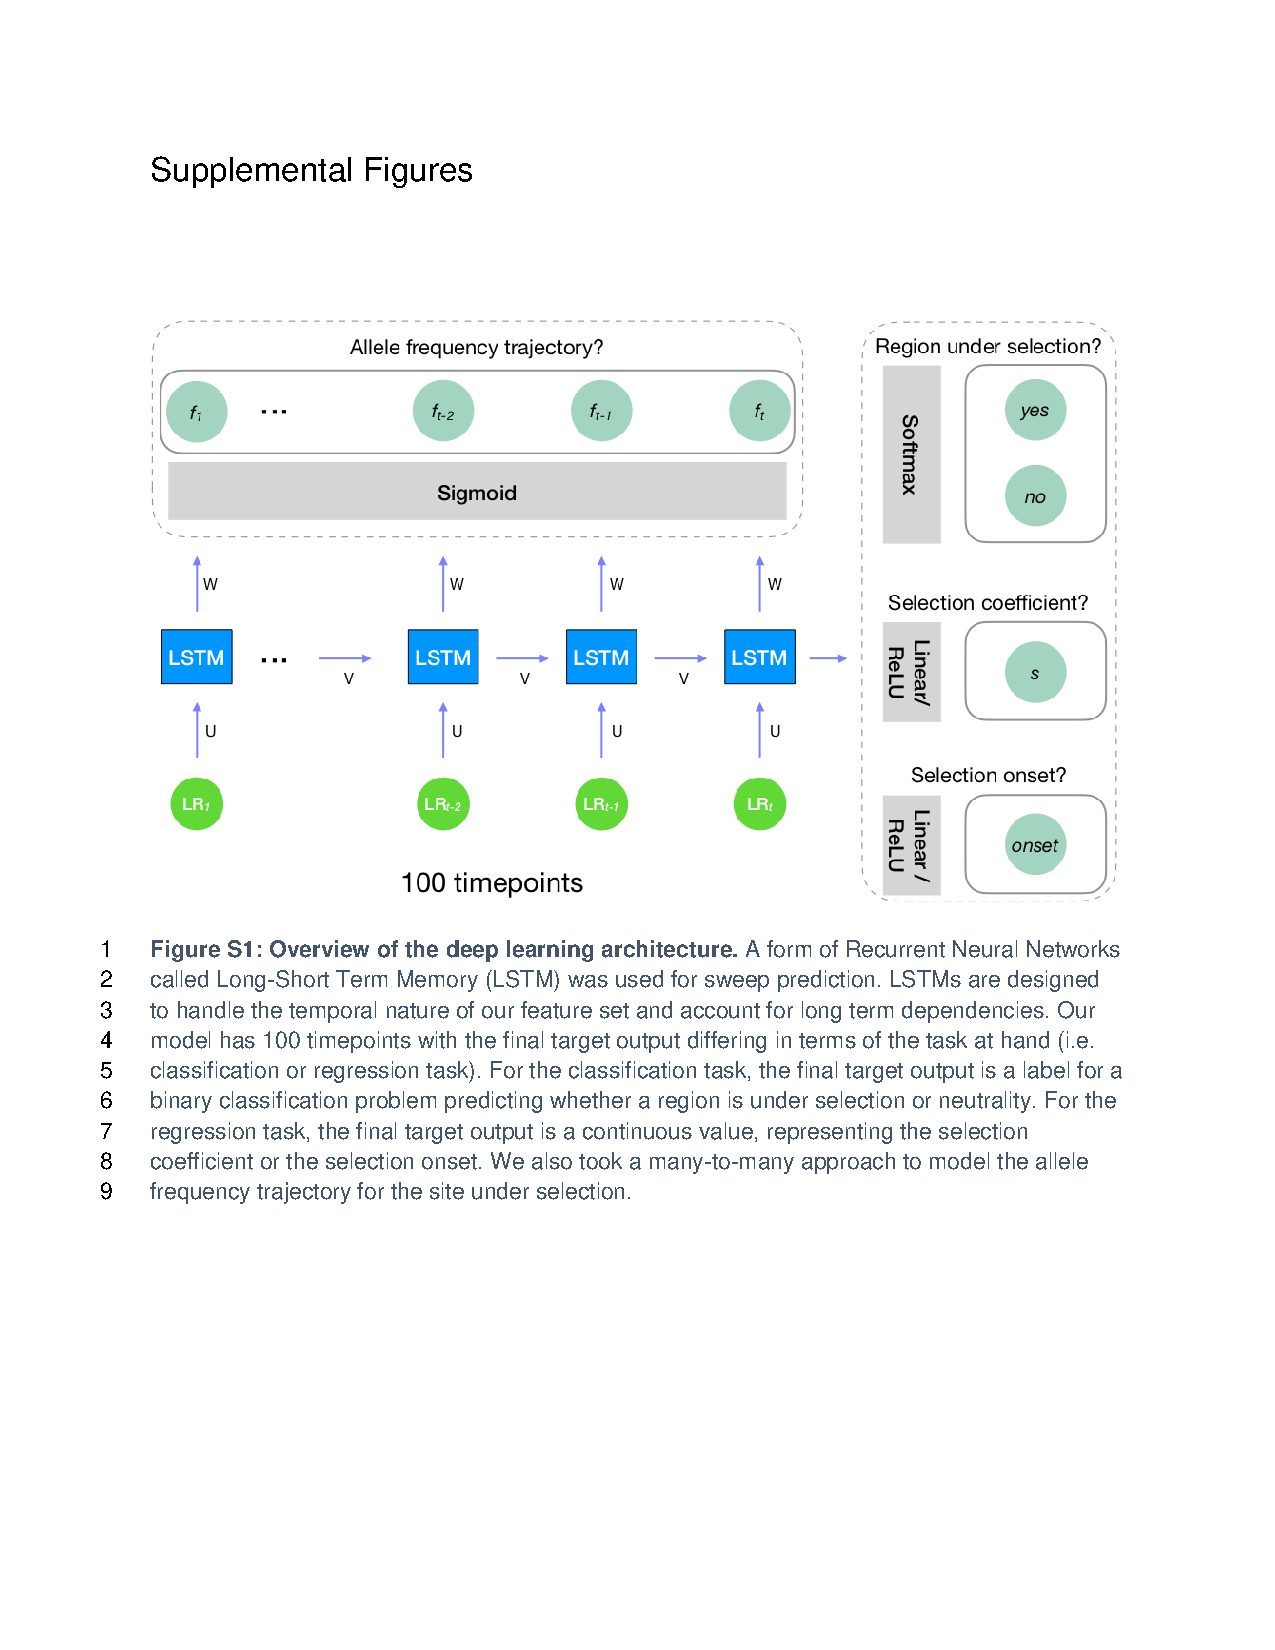
\includepdf[pages=-,scale=0.9,offset=1in -1in,pagecommand={}]{supp/msab332_supp_nopage.pdf}
\chapter{Supplementary material for Chapter \ref{chapter3}} \label{appxB}

The computer code for this project has been deposited in GitHub repos, \href{https://github.com/CshlSiepelLab/bird_capuchino_analysis}{\texttt{bird\_capuchino\_analysis}} and \href{https://github.com/CshlSiepelLab/arg-selection}{\texttt{arg-selection}}. Genomic data have been archived in GenBank (BioProject ID PRJNA835722). Supplementary tables and figures are included in this appendix.

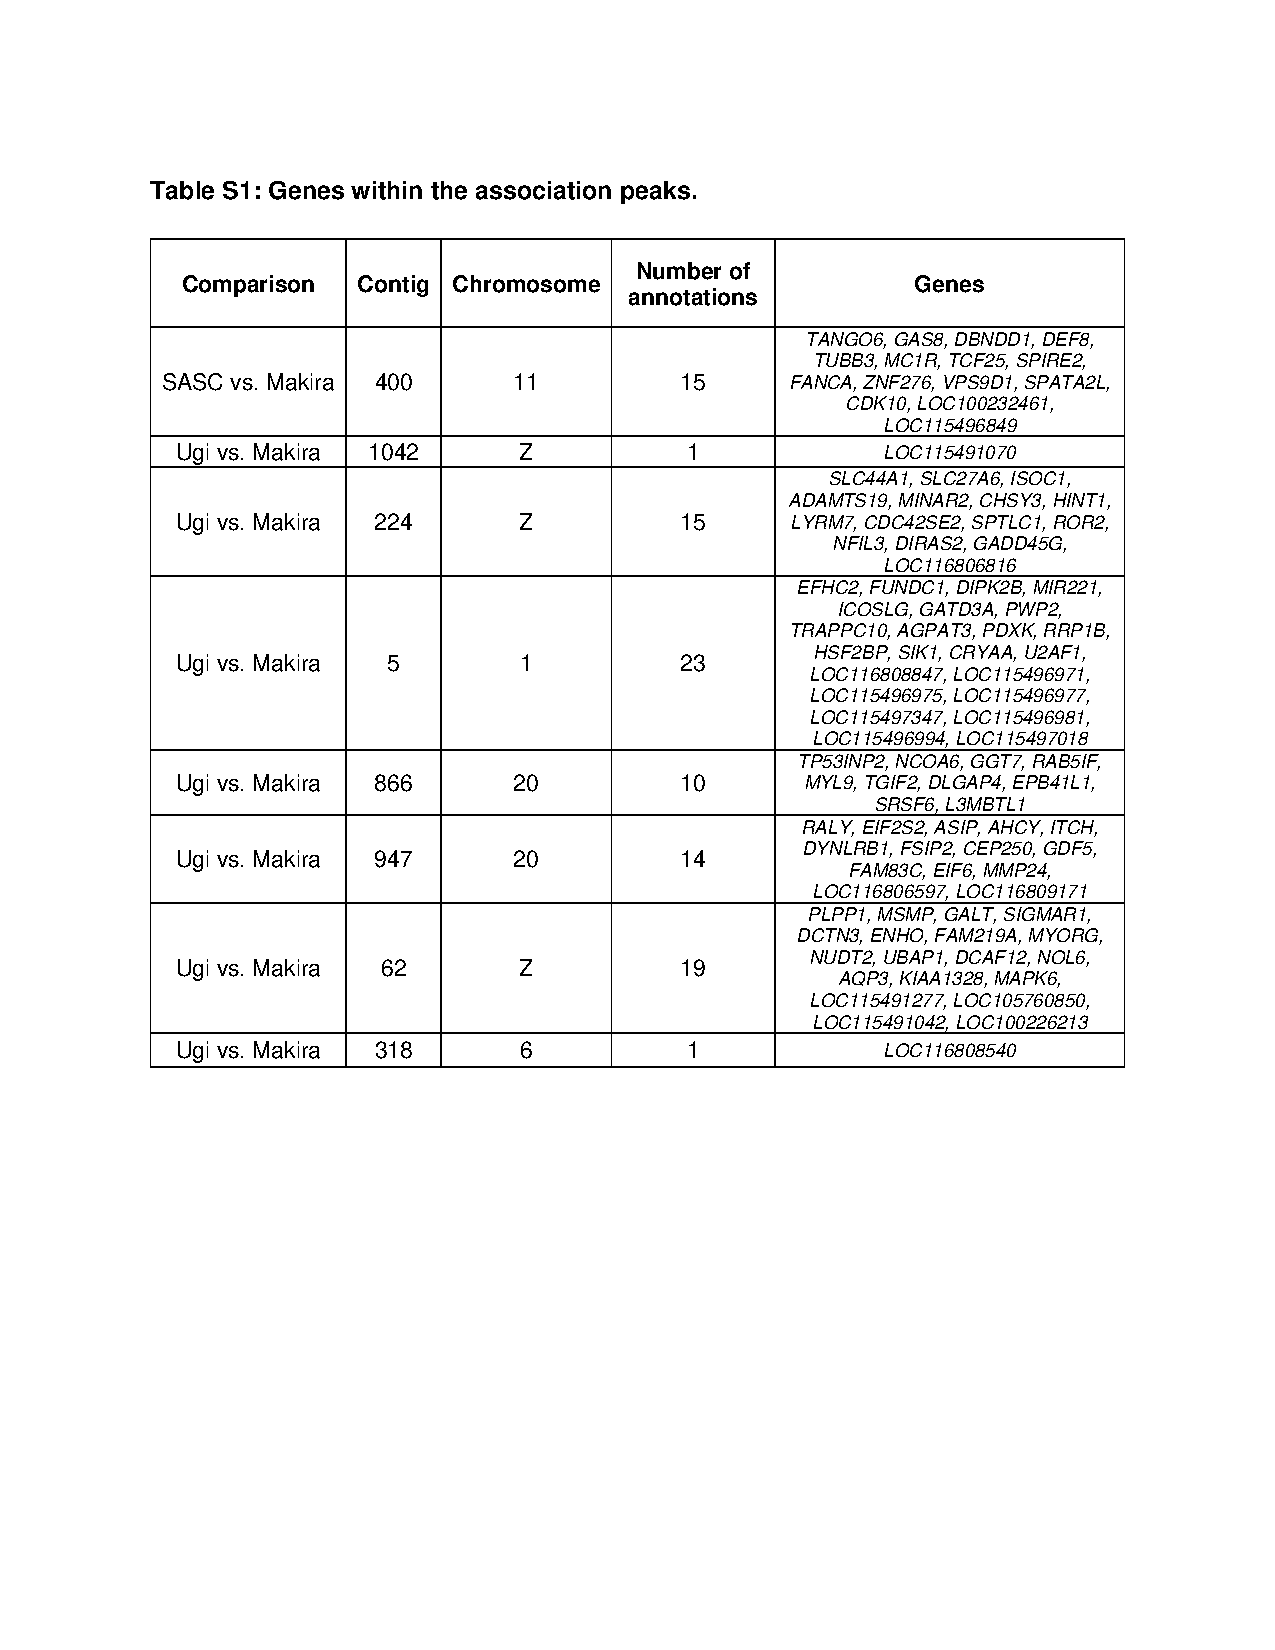
\includepdf[pages=-,scale=0.9,offset=1in -1in,pagecommand={}]{supp/pgen.1010474.supp.pdf}

\chapter{Supplementary material for Chapter \ref{chapter4}} \label{appxC}

All code used in this study are available at \href{https://github.com/ziyimo/popgen-dom-adapt}{GitHub}. The 1000 Genomes data are available \href{https://www.internationalgenome.org/data}{online}. Supplementary figures are included in this appendix.

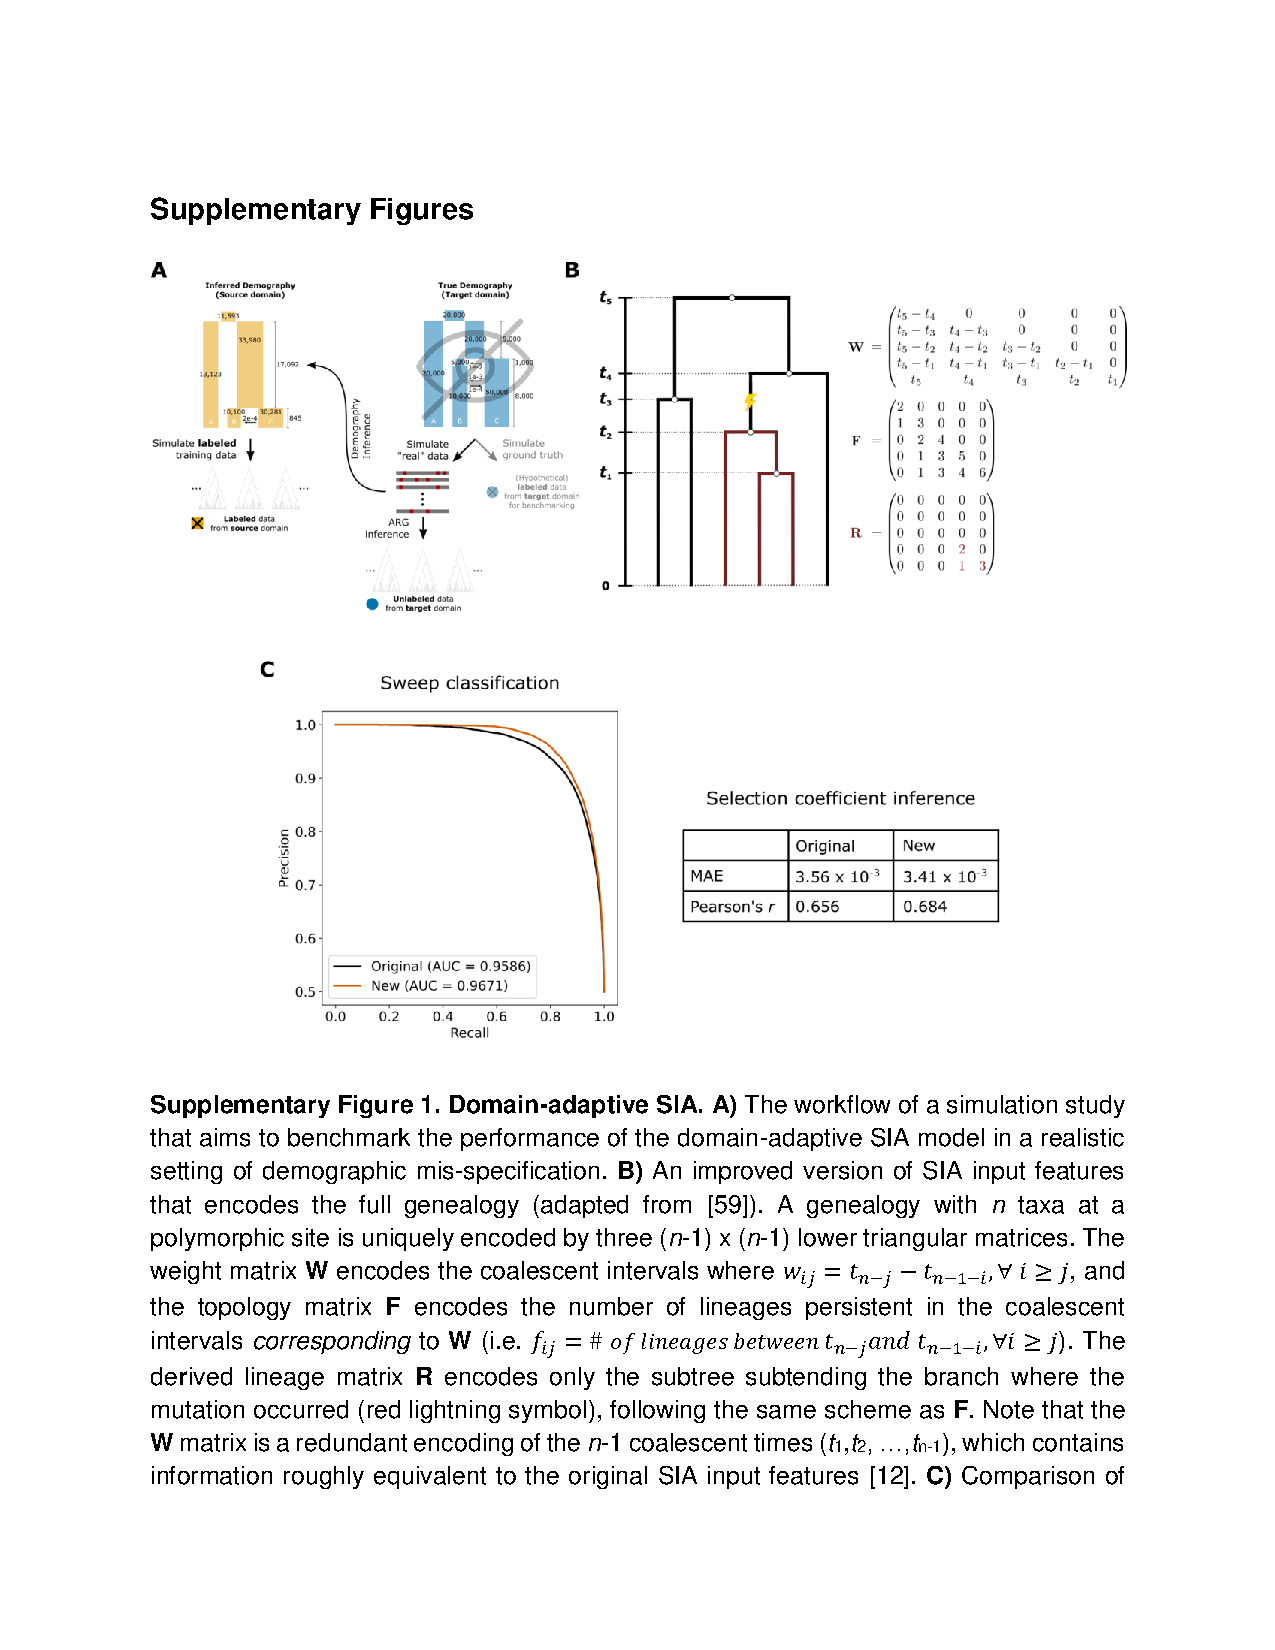
\includepdf[pages=-,scale=0.9,offset=1in -1in,pagecommand={}]{supp/dom-adapt-plos-gen-supp-nopage.pdf}

\end{document}
